\chapter{Modeling 44 Tau and HD 187547}
\label{modeling}
In this chapter the process of modeling the stars 44 Tau and Superstar in \texttt{MESA} and \texttt{GYRE} is described. The methods for comparing the models to  observations is introduced and discussed.

\section{Choosing a grid}
\label{sec:grid}
For this project a grid of models is calculated in order to compare to observations and determine the evolutionary stages of 44 Tau and HD 187547. More than one approach can be taken to reach this goal, each with their own advantages and disadvantages. \citet{lenz2010delta} narrows down the grid size by first calculating the best mass for each stage. It is an approach where the star is initially assumed to be in the MS, post-MS contraction or post-MS expansion phase. This results in three different grids where the best model is found for each stage. This method has the advantage that is it forces a result on all three stages. However, it is a process that requires the grid to be narrowed through several steps, including a separate analysis of the mass range.

In this project a slightly different approach is used. Instead of dividing the models into different stages and narrowing the three grids, a wide grid stretching over the entire instability domain is calculated, and of these the best models are found. To find not only the best overall model, but also consider their tracks and initial input parameter combination, the best model for each track is found. This choice is discussed in \secref{bestmodel}. 

As discussed in \secref{compute}, the input parameters $\alpha_{mlt}$, $\alpha_{ov}$ have a great influence of the further evolution of the star. Other input parameters such as initial abundances and the mass in particular also influence the evolution of the star. Therefore, the input parameters for the initial grid need to be thoughtfully considered.  The grid must be wide enough in parameter space to not only cover the observationally determined parameter space, but adequately beyond this in order to include the uncertainties on the observations.
The mass has not been observationally determined, but since both stars have been classified $\delta$ Sct stars, the mass can be narrowed by the instability strip. Usually this includes stars between 1.5-2.5 \msun. Therefore this mass range is chosen to be from 1.5\msun to 2.2 \msun\footnote{This limit should preferably be 2.5\msun, but was here restricted to 2.2\msun due to lack of time.}. This yields a range of $0.65<X<0.75$ and $0.01<Z<0.03$\footnote{\texttt{MESA} can go much lower, but is chosen to be 0.01 as there is no indication that either of the stars have extreme values for $Z$. The upper limit is $Z= 0.04$, but this caused convergence issues for more tracks. Therefore, it is limited to 0.03 here.}. Numerical results for two different masses and $Z$ can be seen on \figref{diffz}. Here, the red color correspond to masses of $M=1.75M_\odot$ and black lines $M=1.85M_\odot$. The different values of $Z$ are represented with full and dashed lines respectively. There is a clear difference between tracks with different $Z$. Higher values of $Z$ yield a high opacity which blocks the radiation from the inner layers. Hence, stars with higher metallicity will be less luminous. In this case, the luminosity difference is in the order of \lum = 0.2 within the three sigma uncertainties on the luminosity.  It can also be seen from eq. (7.3) in \citet{christensen2008lecture} that $L \\propt \frac{1}{\kappa}$ ($\kappa$ being the opacity.)


\begin{figure}[htbp]
	\centering
	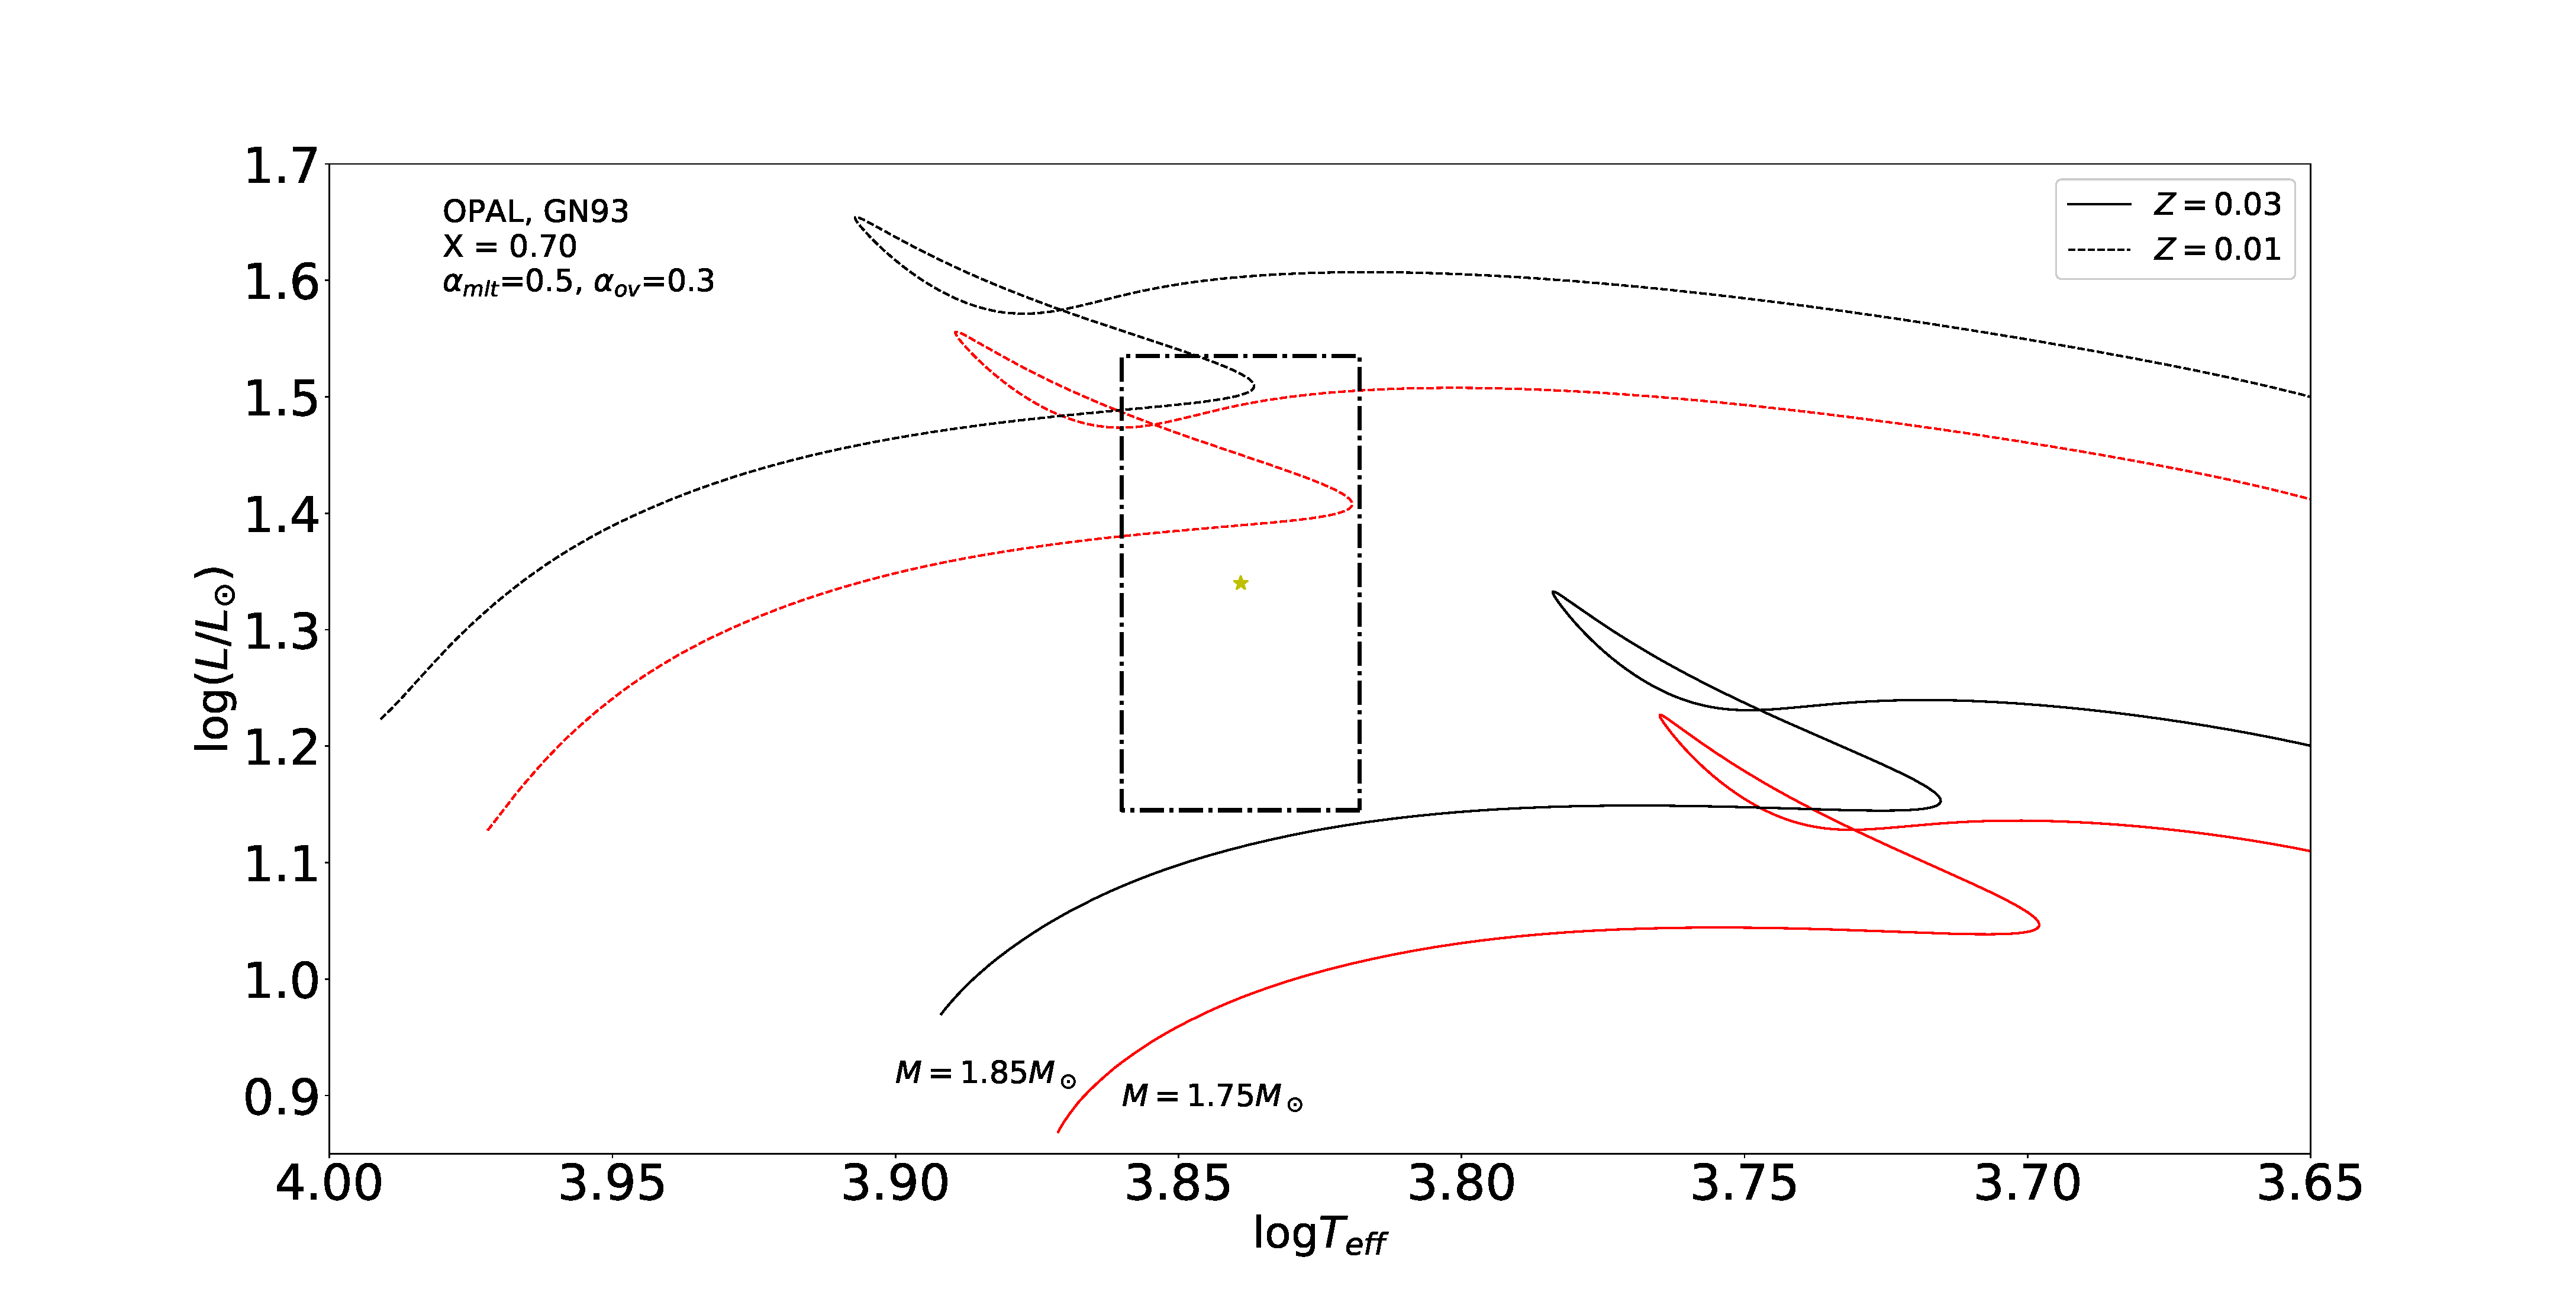
\includegraphics[width=1\textwidth]{test_z.eps}
	\caption{Stellar evolution tracks for two different masses with two different metal abundances. Each track has $X=0.70$, $\alpha_{mlt}=0.5$ and $\alpha_{ov}=0.3$. The red lines indicates tracks with masses of $M=1.75M_\odot$, and black lines indicate $M=1.85M_\odot$. The full lines have $Z = 0.03$ and dashed lines $Z = 0.01$. The black dashed box shows the three sigma uncertainties on \lum and \teff (from \citet{lenz2010delta}). }
	\label{diffz}
\end{figure}

Numerical results for increasing initial abundances at fixed metallicity can be seen in \figref{diffx}. The line and color convention corresponds to that of \figref{diffz}, with the difference being the line type indicating the values of $X$ instead. Here it is also clear that the initial hydrogen abundance affects the luminosity. Higher hydrogen abundances causes $\kappa$ to increase, hence decreasing \lum.

\begin{figure}[htbp]
	\centering
	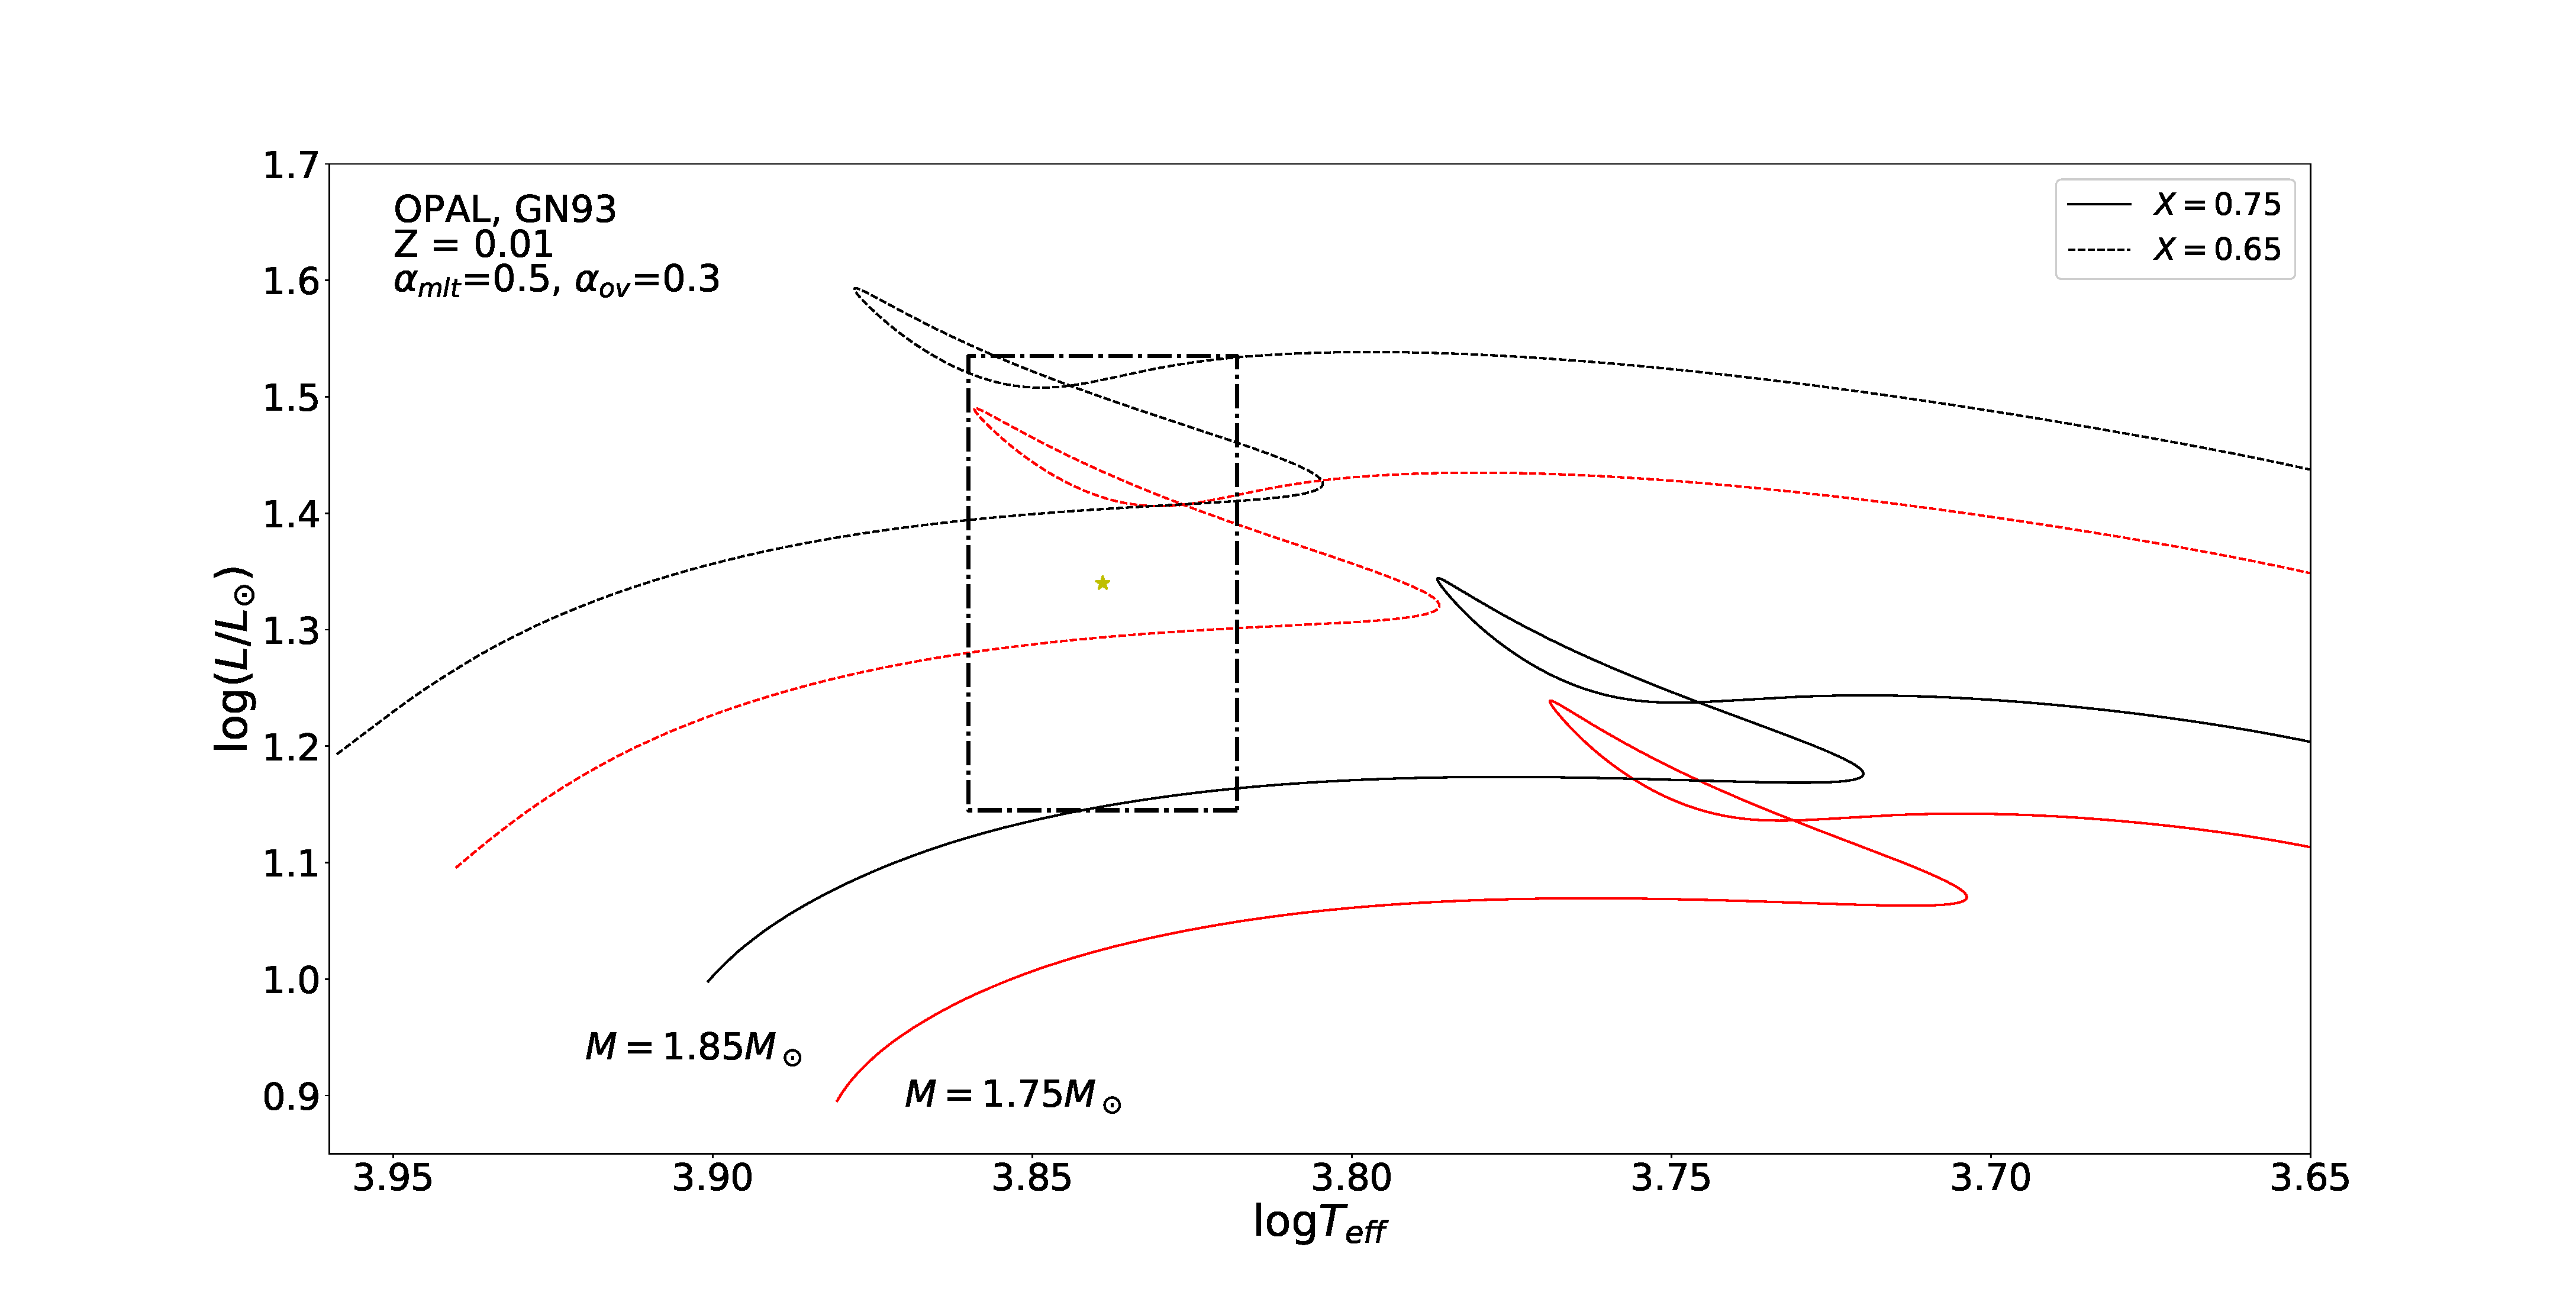
\includegraphics[width=1\textwidth]{test_x.eps}
	\caption{Stellar evolution tracks for two different masses with two different metal abundances. Each track has $Z=0.01$, $\alpha_{mlt}=0.5$ and $\alpha_{ov}=0.3$. The red lines indicates tracks with masses of $M=1.75M_\odot$, and black lines indicate $M=1.85M_\odot$. The full lines have $X = 0.75$ and dashed lines $X = 0.65$. The black dashed box indicates the three sigma uncertainties on \lum and \teff (from \citet{lenz2010delta}).}
	\label{diffx}
\end{figure}

 Parameters $\alpha_{mlt}$ and $\alpha_{ov}$ difficult to establish, since they are purely empirical and depend strongly on the prescription used in the modeling (see \secref{sec:conv_prescriptions}. For the $\alpha_{mlt}$ the standard value in \texttt{MESA} is around 1.8. The Warsaw-New Jersey stellar evolution code used to calculate models for 44 Tau by \citet{lenz2010delta} has a mixing length prescription bases on the standard mixing length theory like \texttt{MESA}. Their results showed that models with mixing length of $\alpha_{mlt} > 0.2$ gave the best fits, confirming the assumption that smaller mixing lengths than the sun is needed in order to model these stars. However, \texttt{MESA} is not computationally capable of handling a mixing length below 0.2 which is not surprising as it would mean that energy transport by convection in the outer layers is almost non existing in the  \texttt{MESA} implementation. This also underlines the fact that convection is treated differently in each stellar evolution code through the implementation of $\alpha_{mlt}$(as discussed in \chapref{compute}), which therefore needs to be carefully evaluated in the grid. It can also be argued that since $\delta$ Sct stars have a significantly smaller convection layer than that of the Sun, the convection will not be as efficient.  \citet{trampedach2011mass} calculated a range of mixing lengths through a grid simulation of solar type structures. One of the results can be seen on \figref{tramp}. 

\begin{figure}[htbp]
	\centering
	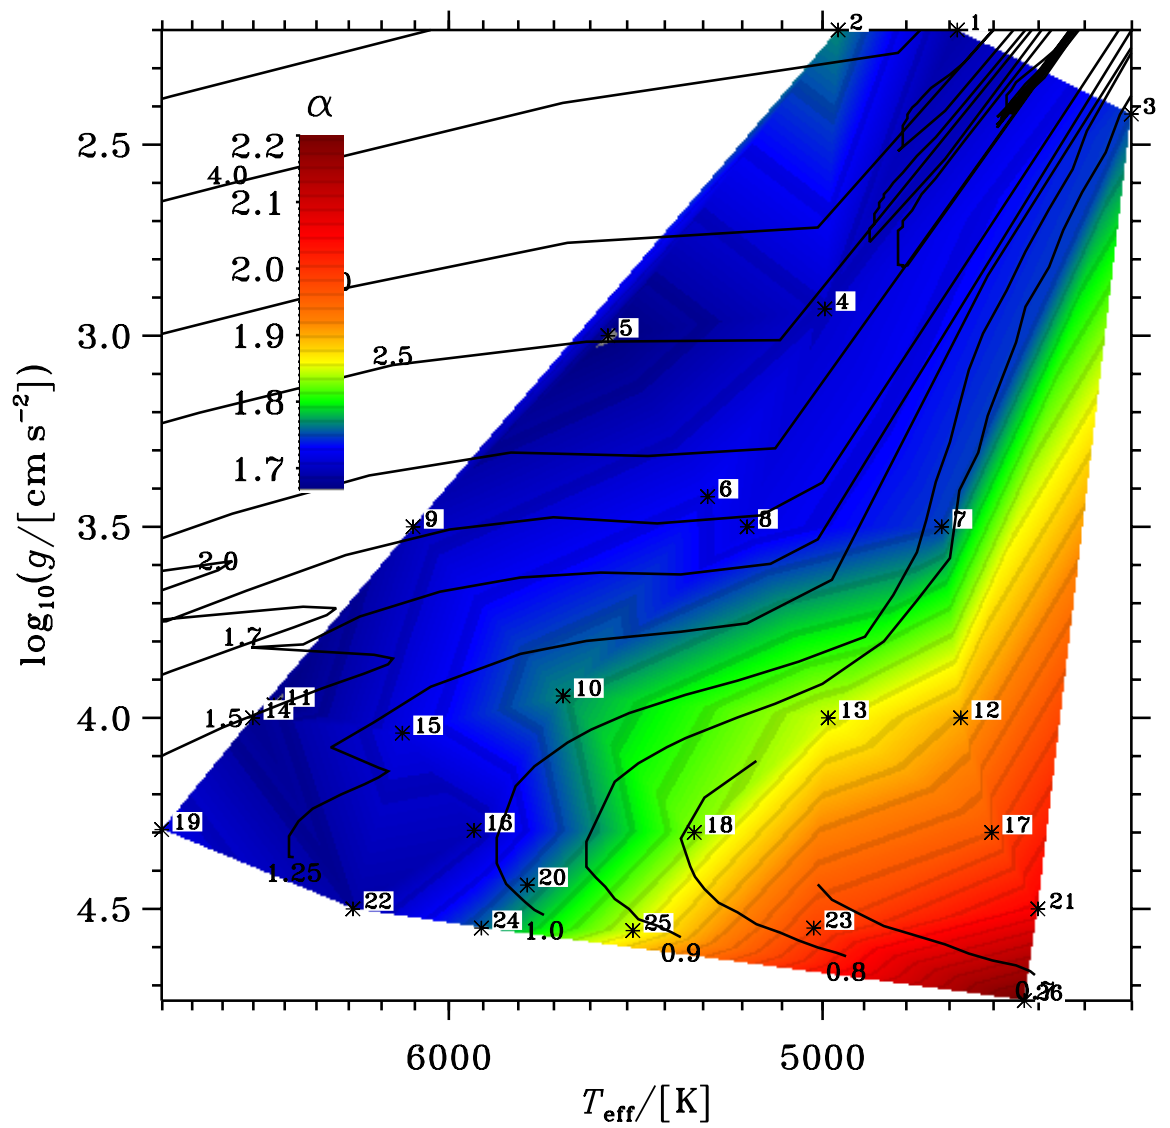
\includegraphics[width=0.8\textwidth]{tramper.png}
	\caption{Mass mixing lengths in units of pressure scale height $H_p$ in the \teff - $\log g$ plane. From \citep{trampedach2011mass}.}
	\label{tramp}
\end{figure}

The mixing length is predicted to be smaller for higher values of \teff, as expected. Both 44 Tau and HD 187547 are out of range in \teff space, since the mixing length range here is calculated based on solar-like structures. However, the trend in mixing length is still applicable to the stars in this work. As an initial grid, values of $\alpha_{mlt}$ between 0.2 and 0.8 are chosen. Analogous to the mixing length, the convective overshoot near the core is described with the convective core overshoot parameter $\alpha_{ov}$. As it is typically in the order of 0.1-0.2 \citep{kippenhahn1990stellar}, values between 0.1-0.3 are chosen.  The initial grid used here can be seen in \tabref{grid}.
\begin{table}[htbp]
  \centering
  \caption{Values and step sizes for all parameters in the grid calculated in this work. }
  \label{grid}
  \begin{tabular}{lll}\toprule
    & values    & step size \\ \midrule
    X                         & 0.65-0.75 & 0.05     \\
    Z                         & 0.01-0.03 & 0.01     \\
    Mass/\msun                & 1.5-2.2   & 0.05     \\
    $\alpha_{mlt}$            & 0.2-0.8   & 0.3      \\
    $\alpha_{ov}$             & 0.1-0.3   & 0.1      \\ \bottomrule
    \end{tabular}
\end{table}

Some of these combinations did however not converge properly, and could therefore not be included in the grid. These models are:
\begin{itemize}
	\item $M=1.50M_\odot$: combinations with $X=0.75$ and $Z=0.02$ or $Z=0.03$
	\item $M=1.55M_\odot$: combinations with $X=0.75$ and $Z=0.03$
	\item $M=1.95M_\odot$: combinations with $X=0.75$ and $Z=0.03$
	\item $M=1.80M_\odot$: combinations with $X=0.75$ and $Z=0.02$ and $\alpha_{mlt} = 0.2$
	\item $M=1.90M_\odot$: combinations with $X=0.75$ and $Z=0.02$ and $\alpha_{mlt} = 0.8$ 
\end{itemize}

It is unclear why these exact combinations have numerical issues, and further investigation needs to be done. Some of these combinations lead to extreme helium abundances , particularly the case where $X=0.75$ and $Z=0.03$ yielding $Y=0.22$. This might explain most of the issues since this value is lower than the primordial helium abundance. Likewise, the combination of  $X=0.65$, $Z=0.0.1$ yields $Y=0.31$ which might only be observed in strange cases. The reason for still including these extreme values is that models might still be able to reproduce these numbers in the calculation. So if a model has this value it can be interpreted as an example of the imperfect theory behind the stellar structure an evolution codes.  

\section{Resolution and varcontrol}
\label{sec:res}

As mentioned previously in \secref{sec:mesa}, they way \texttt{MESA} works is to fulfill calculations in time steps that are non-equidistant. As a result of this, models on a track can be far apart, particularly if the evolution is fast. This means that models on the MS are well resolved, while the models on fast stages (particularly post-MS contraction phase) are far apart in terms of structure. This also results in the frequencies being very different from one model to another, which should be considered when calculating the \chis (see \secref{sec:chis}). An example can be seen on \figref{resstage} where, the radial fundamental mode is plotted as a function of timestep. The upper panel shows an HRD with the evolution divided into three stages MS (1), post-MS contraction (2), and post-MS expansion (3). The lower panel of \figref{resstage} is the same models corresponding to middle panel but where the radial fundamental mode frequency difference between models, $f_1(i+1) - f_1(i)$, is plotted as a function of time. This shows that the resolution in the frequency space is as high as ~0.18 $d^{-1}$ for this track\footnote{Some tracks have poorer resolution of ~0.2$d^{-1}$}. The highest point is on the MS which should be taken into account for HD 187547. For 44 Tau, the focus for the resolution control should be much later on the post-MS.      

\begin{figure}[htbp]
    \centering
    %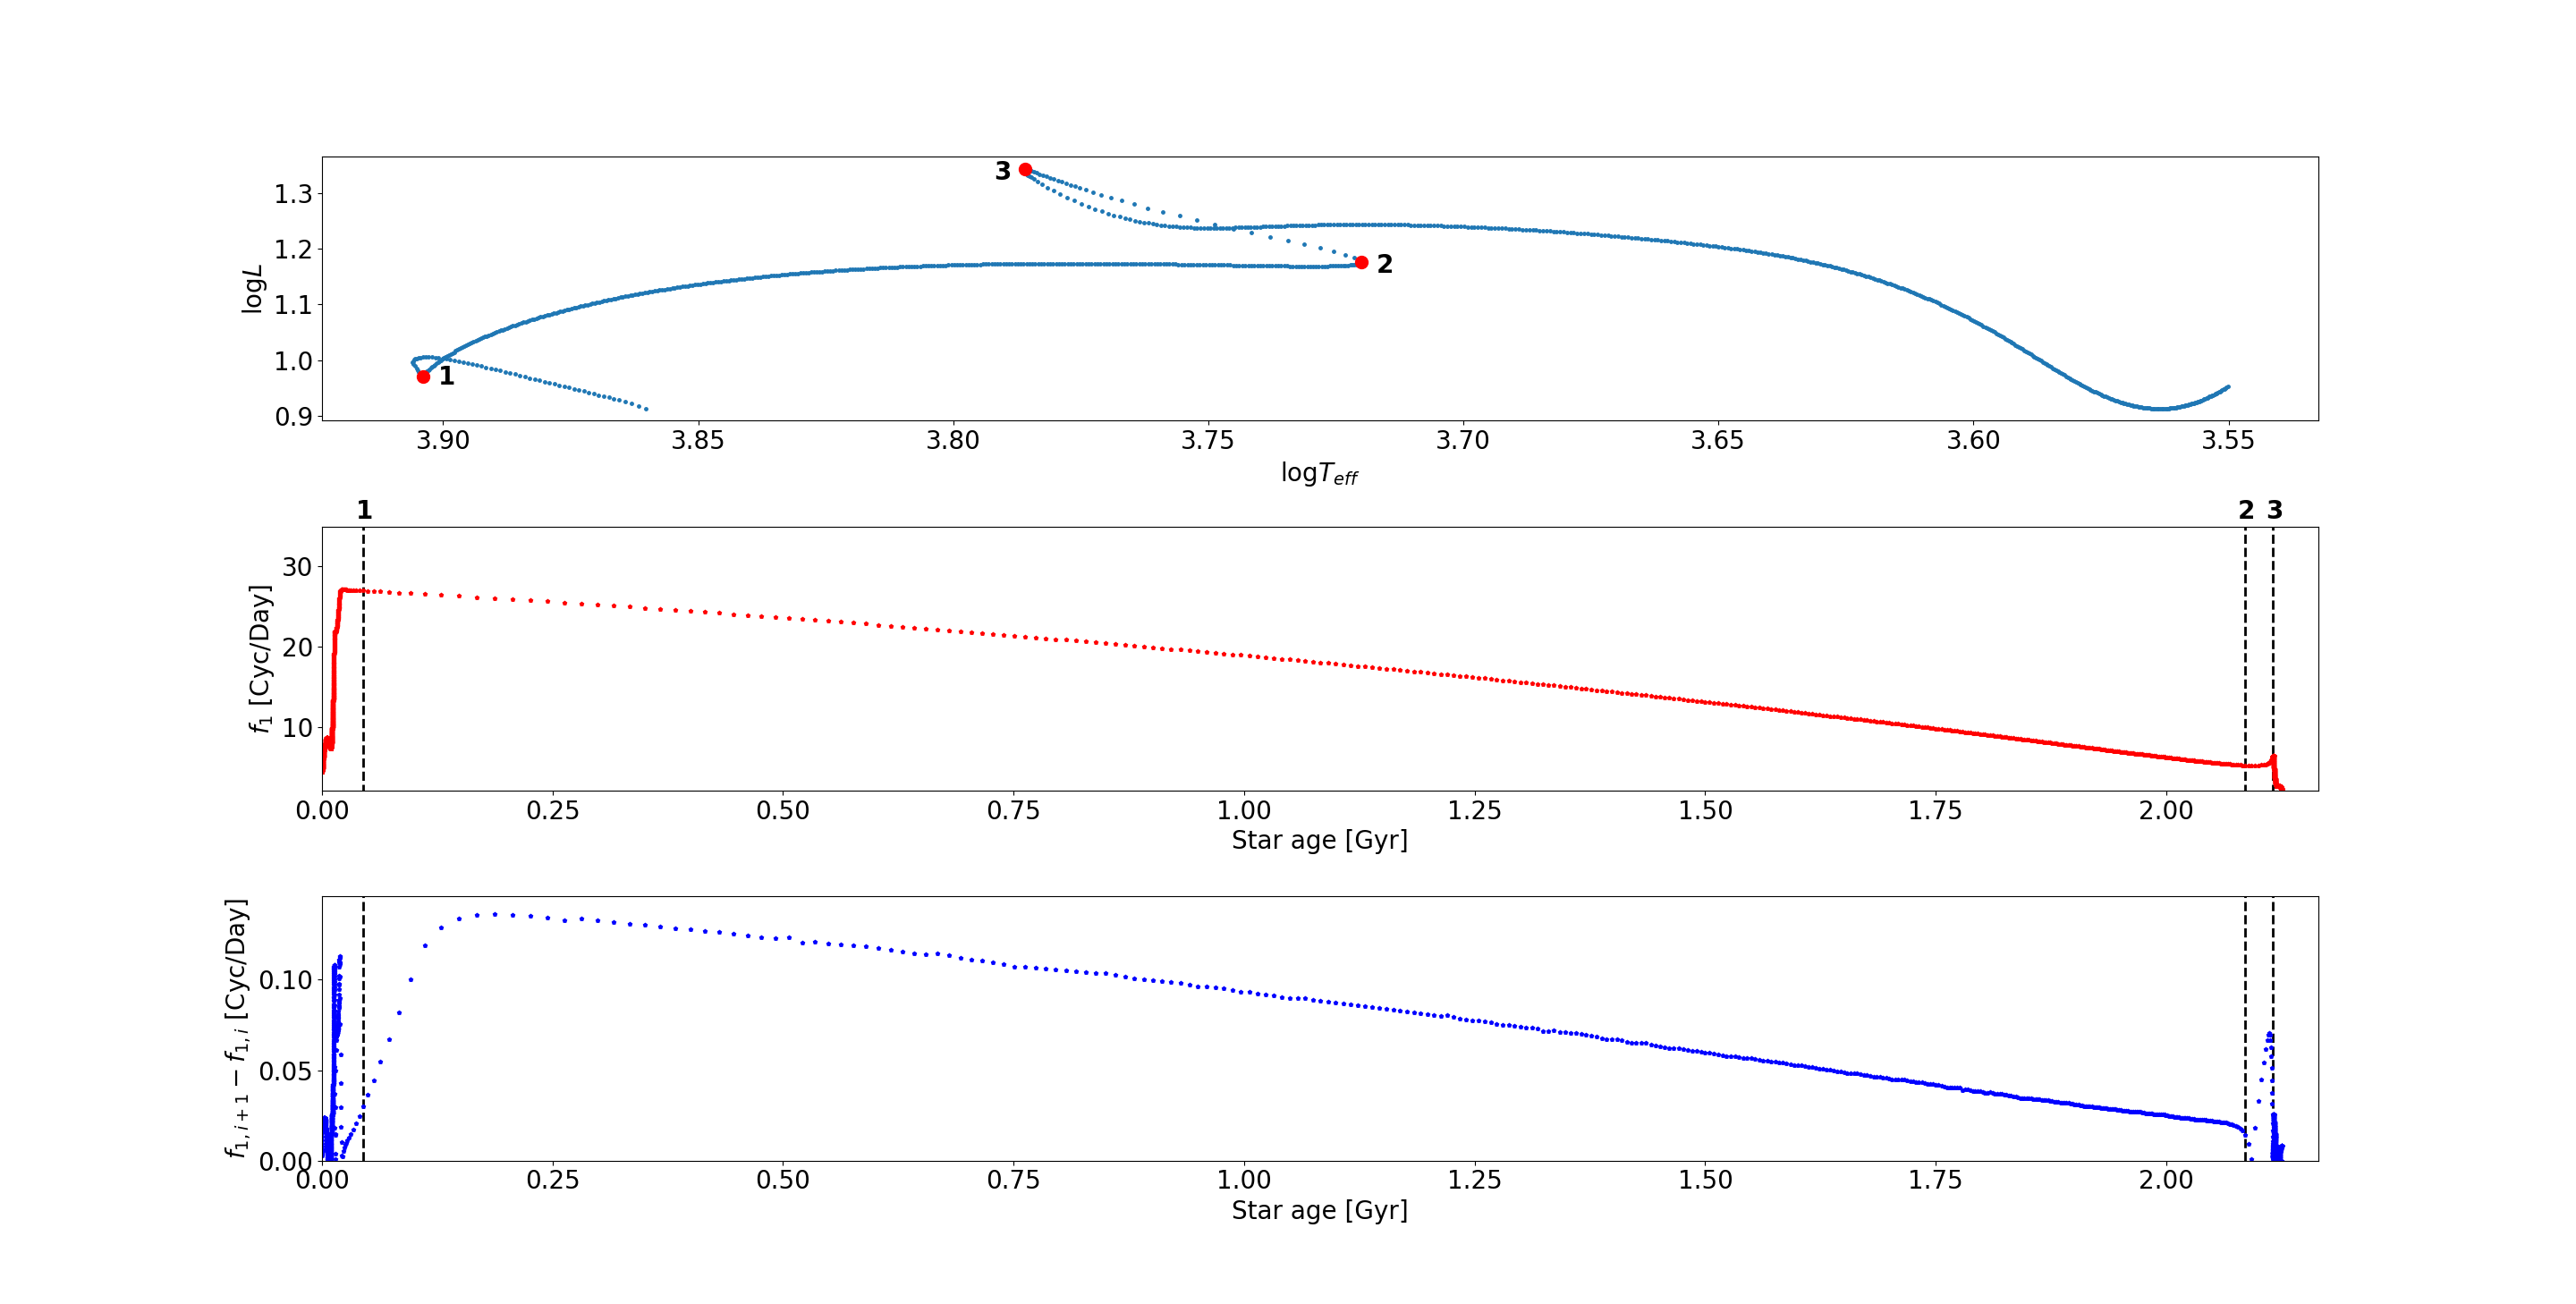
\includegraphics[width=1\textwidth]{resolution_stages.png}
    	\makebox[\textwidth][c]{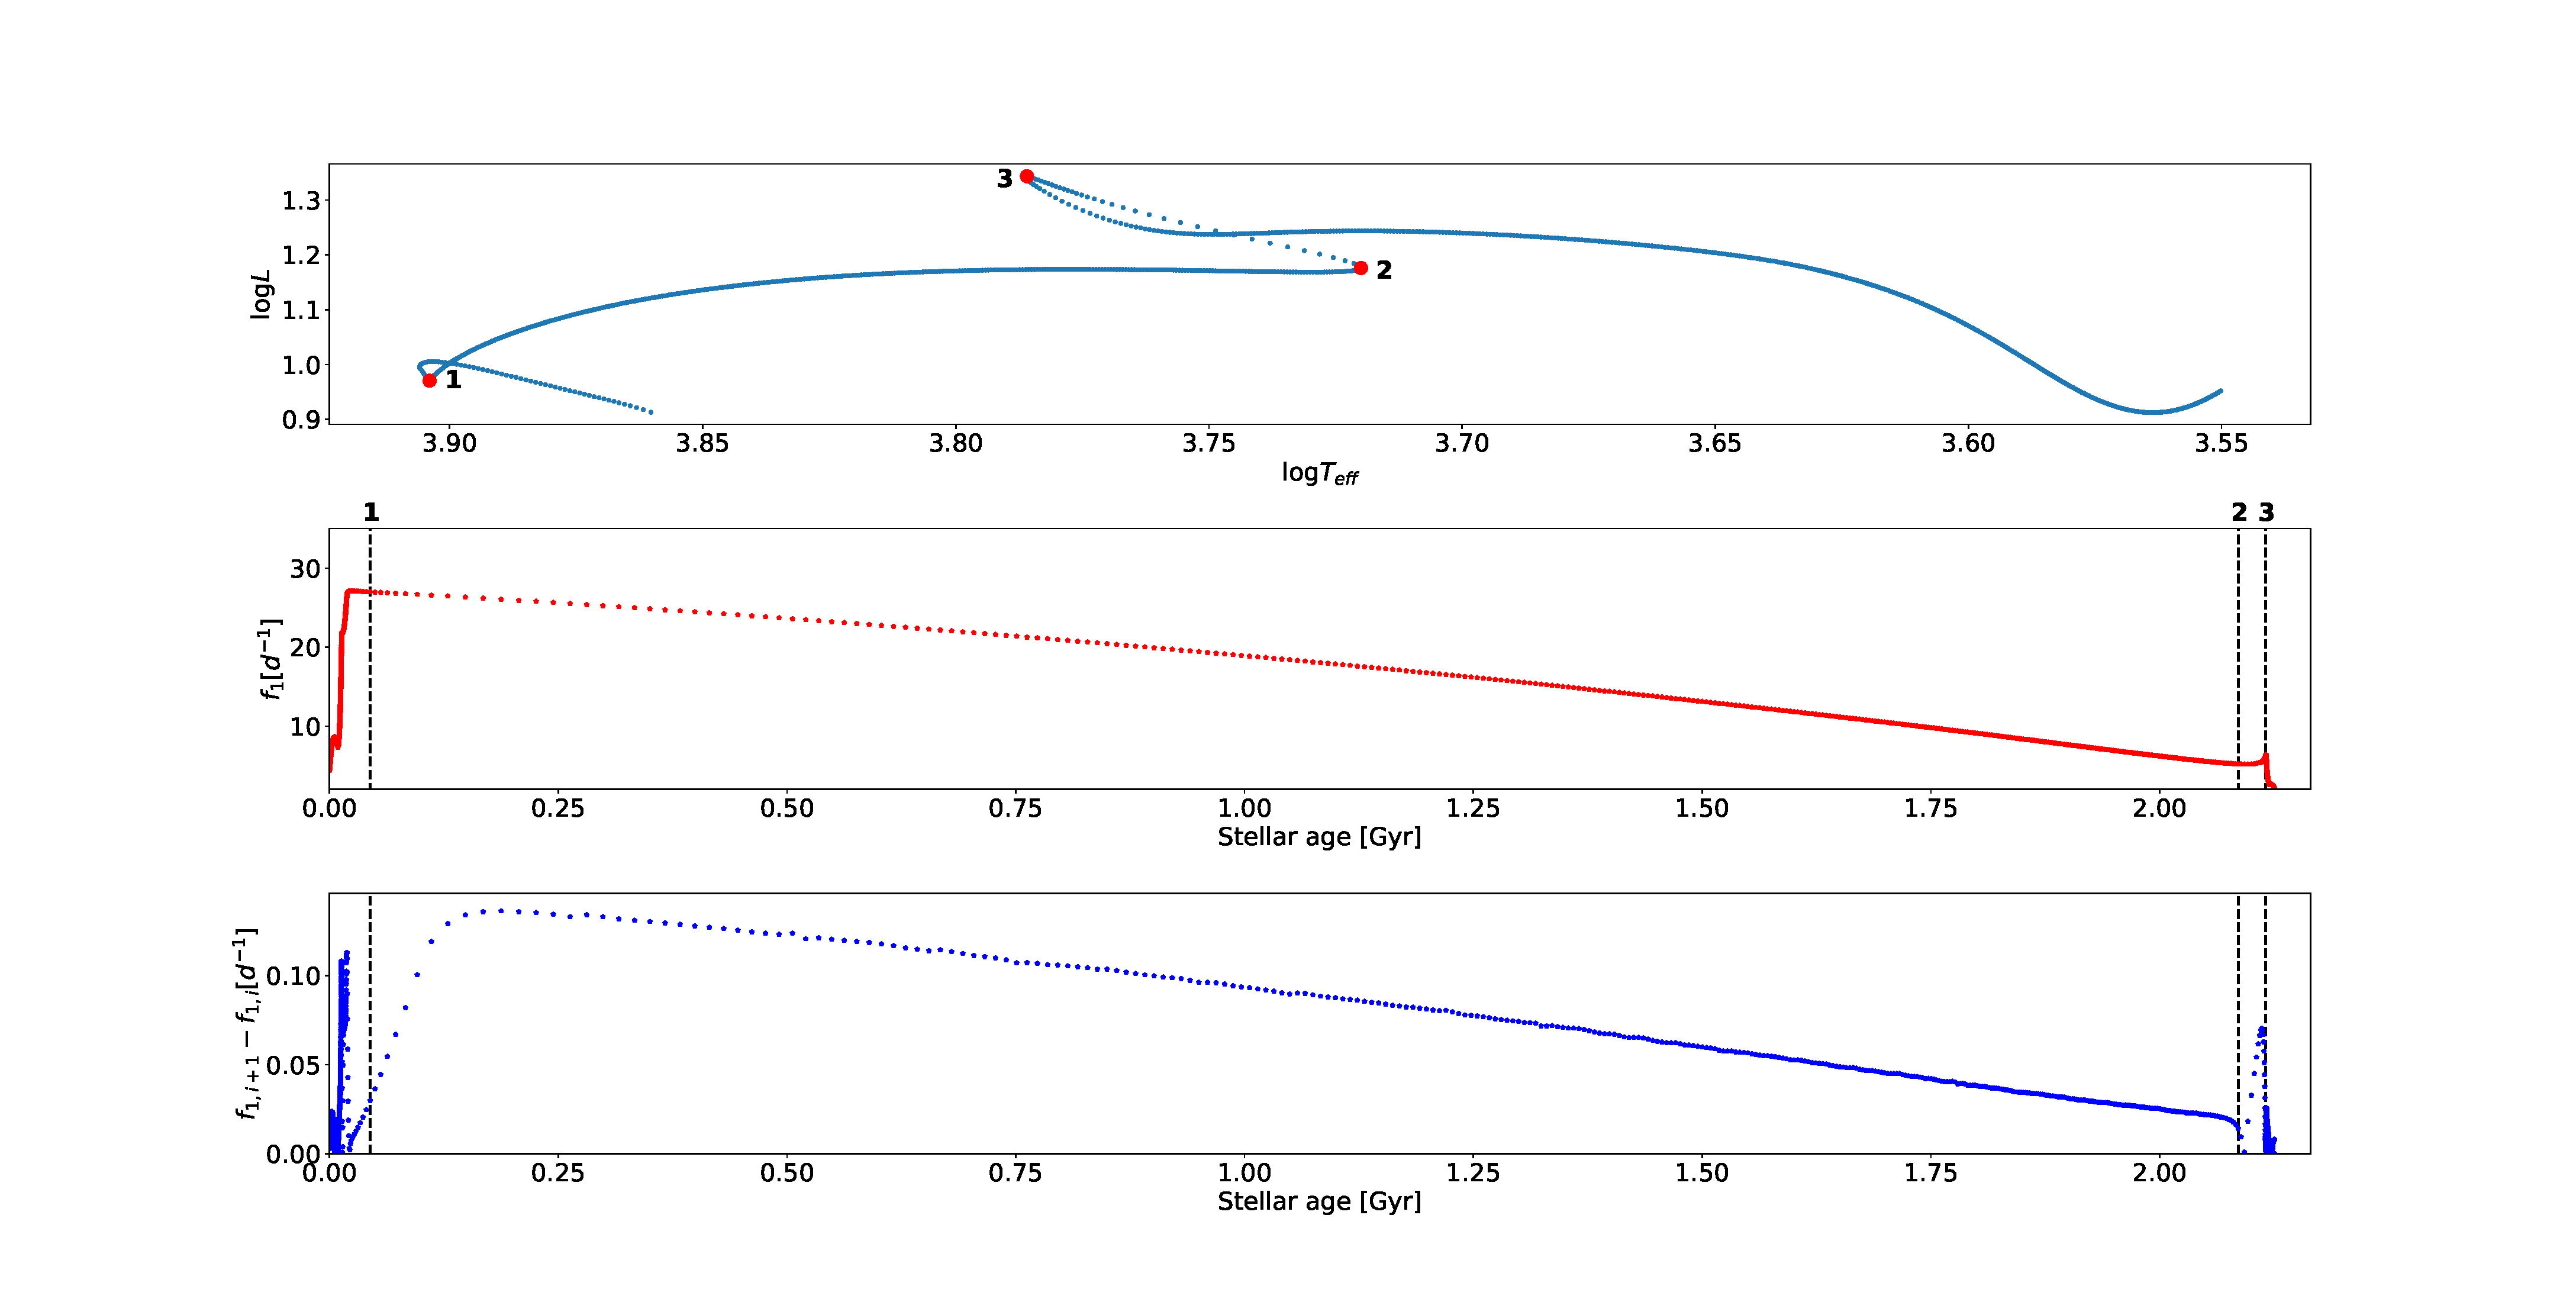
\includegraphics[width=1\textwidth]{freqsplot.eps}}%
    \caption{Resolution at different stages of an evolution of a track with M=1.85\msun, X=0.75, Z=0.02, $\alpha_{mlt} = 0.5$, $\alpha_{ov} = 0.3$. The beginning of the MS is marked with a bold "1", continuing until "2" where the post-MS contraction phase starts. At "3" all hydrogen has been exhausted in the core, and the star is in the post-MS expansion phase. Middle panel: Here the fundamental frequency is plotted as a function of time. The dashed lines indicate the stages corresponding to those in the middle panel. Lower panel: Shows the absolute difference in fundamental frequency between two subsequent models.}
    \label{resstage}
\end{figure}

Since 44 Tau has earlier been identified to be in the post-MS phase and the low value of \lum for HD 187547 indicates an earlier stage on MS, the resolution of the models in \texttt{MESA} needs to be adjusted to allow for a higher chance of finding a good fit, particularly within these stages. It is possible to simply force smaller time steps, but this is not ideal since it would not only increase the computation time on the fast evolutionary stages, but the entire track. It is therefore favorable to consider an alternative parameter that does not spend computation in areas where it is not needed. 

There are more than one way of achieving this. It is possible to set a limit for magnitude of maximum change in temperature and photosphere with the \texttt{delta\_lgTeff\_limit}, or alter the minimum and maximum number of grid points in a model with \texttt{mesh\_delta\_coeff} (a higher value decreases the number). The parameter found to be most efficient in this project is the \texttt{varcontrol\_target} parameter. This parameter is assigned a value describing the relative variation in the structure from one model to the next. The timestep then adjusts accordingly, depending on whether the variation is smaller or larger than the value. Increasing the resolution through this value does also increase the computation time. An example of this can be seen on \figref{varcontrol} where the same track is plotted with different values of \texttt{varcontrol\_target}. It is here found that a value of $5\cdot10^{-5}$ is sufficient in making the resolution satisfactory for this work. 

\begin{figure}[htbp]
    \centering
   % 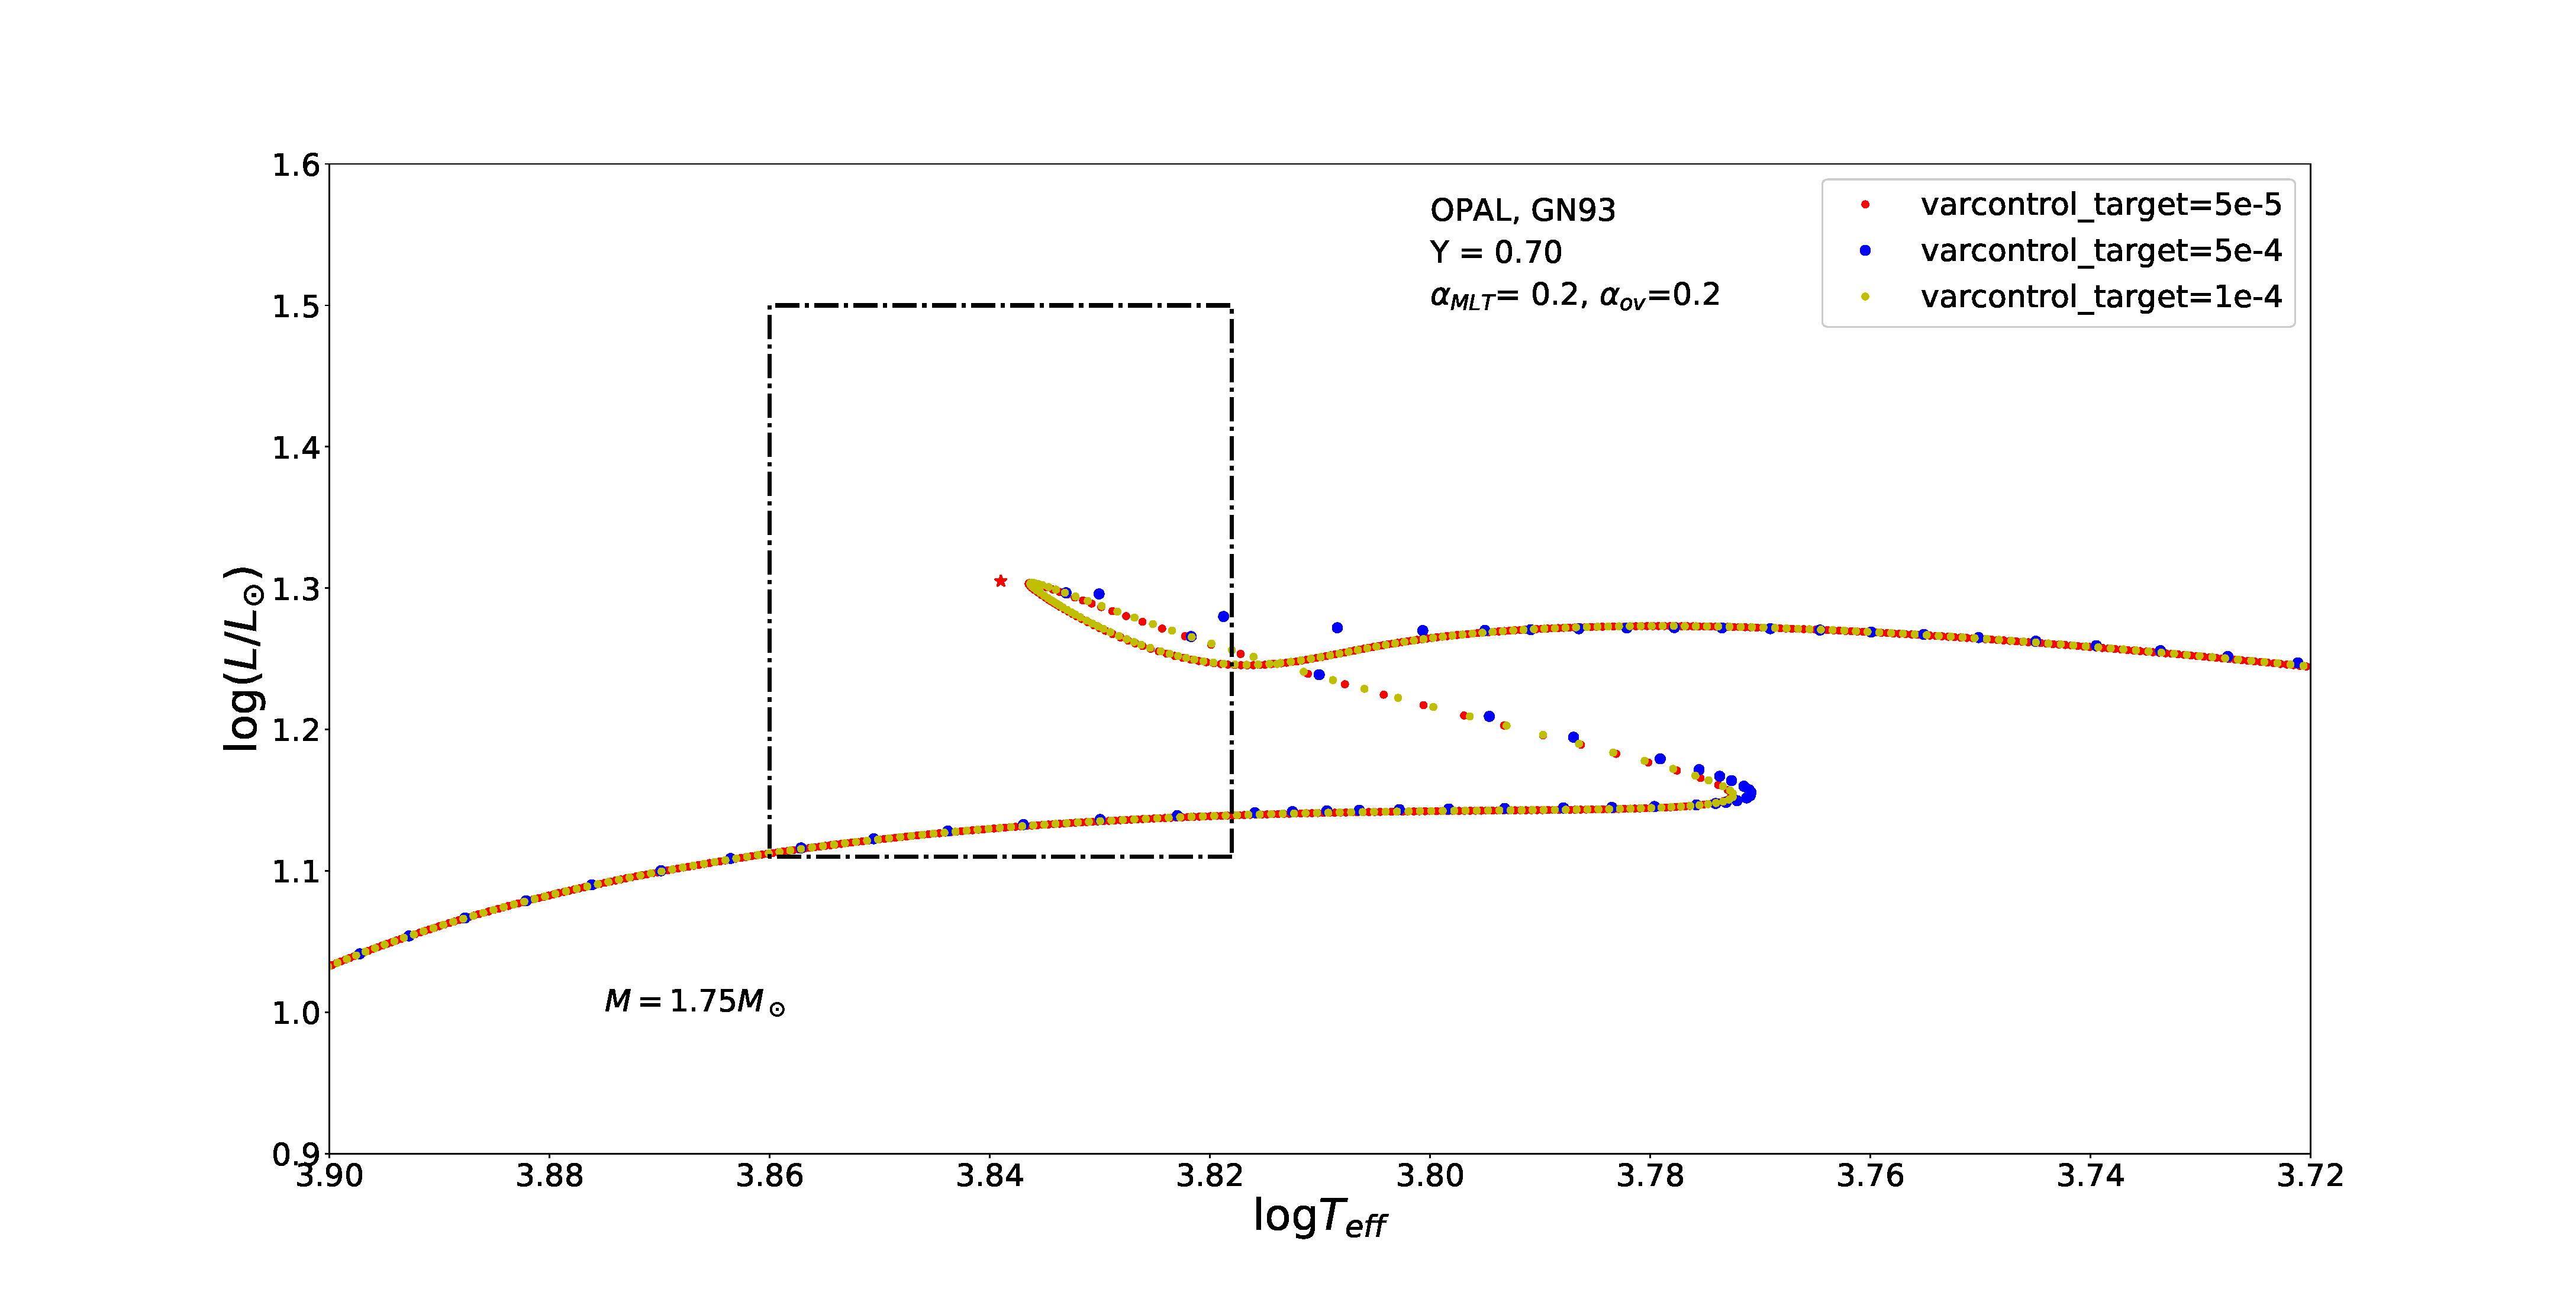
\includegraphics[width=1\textwidth]{varcontrol_res.eps}
   	\makebox[\textwidth][c]{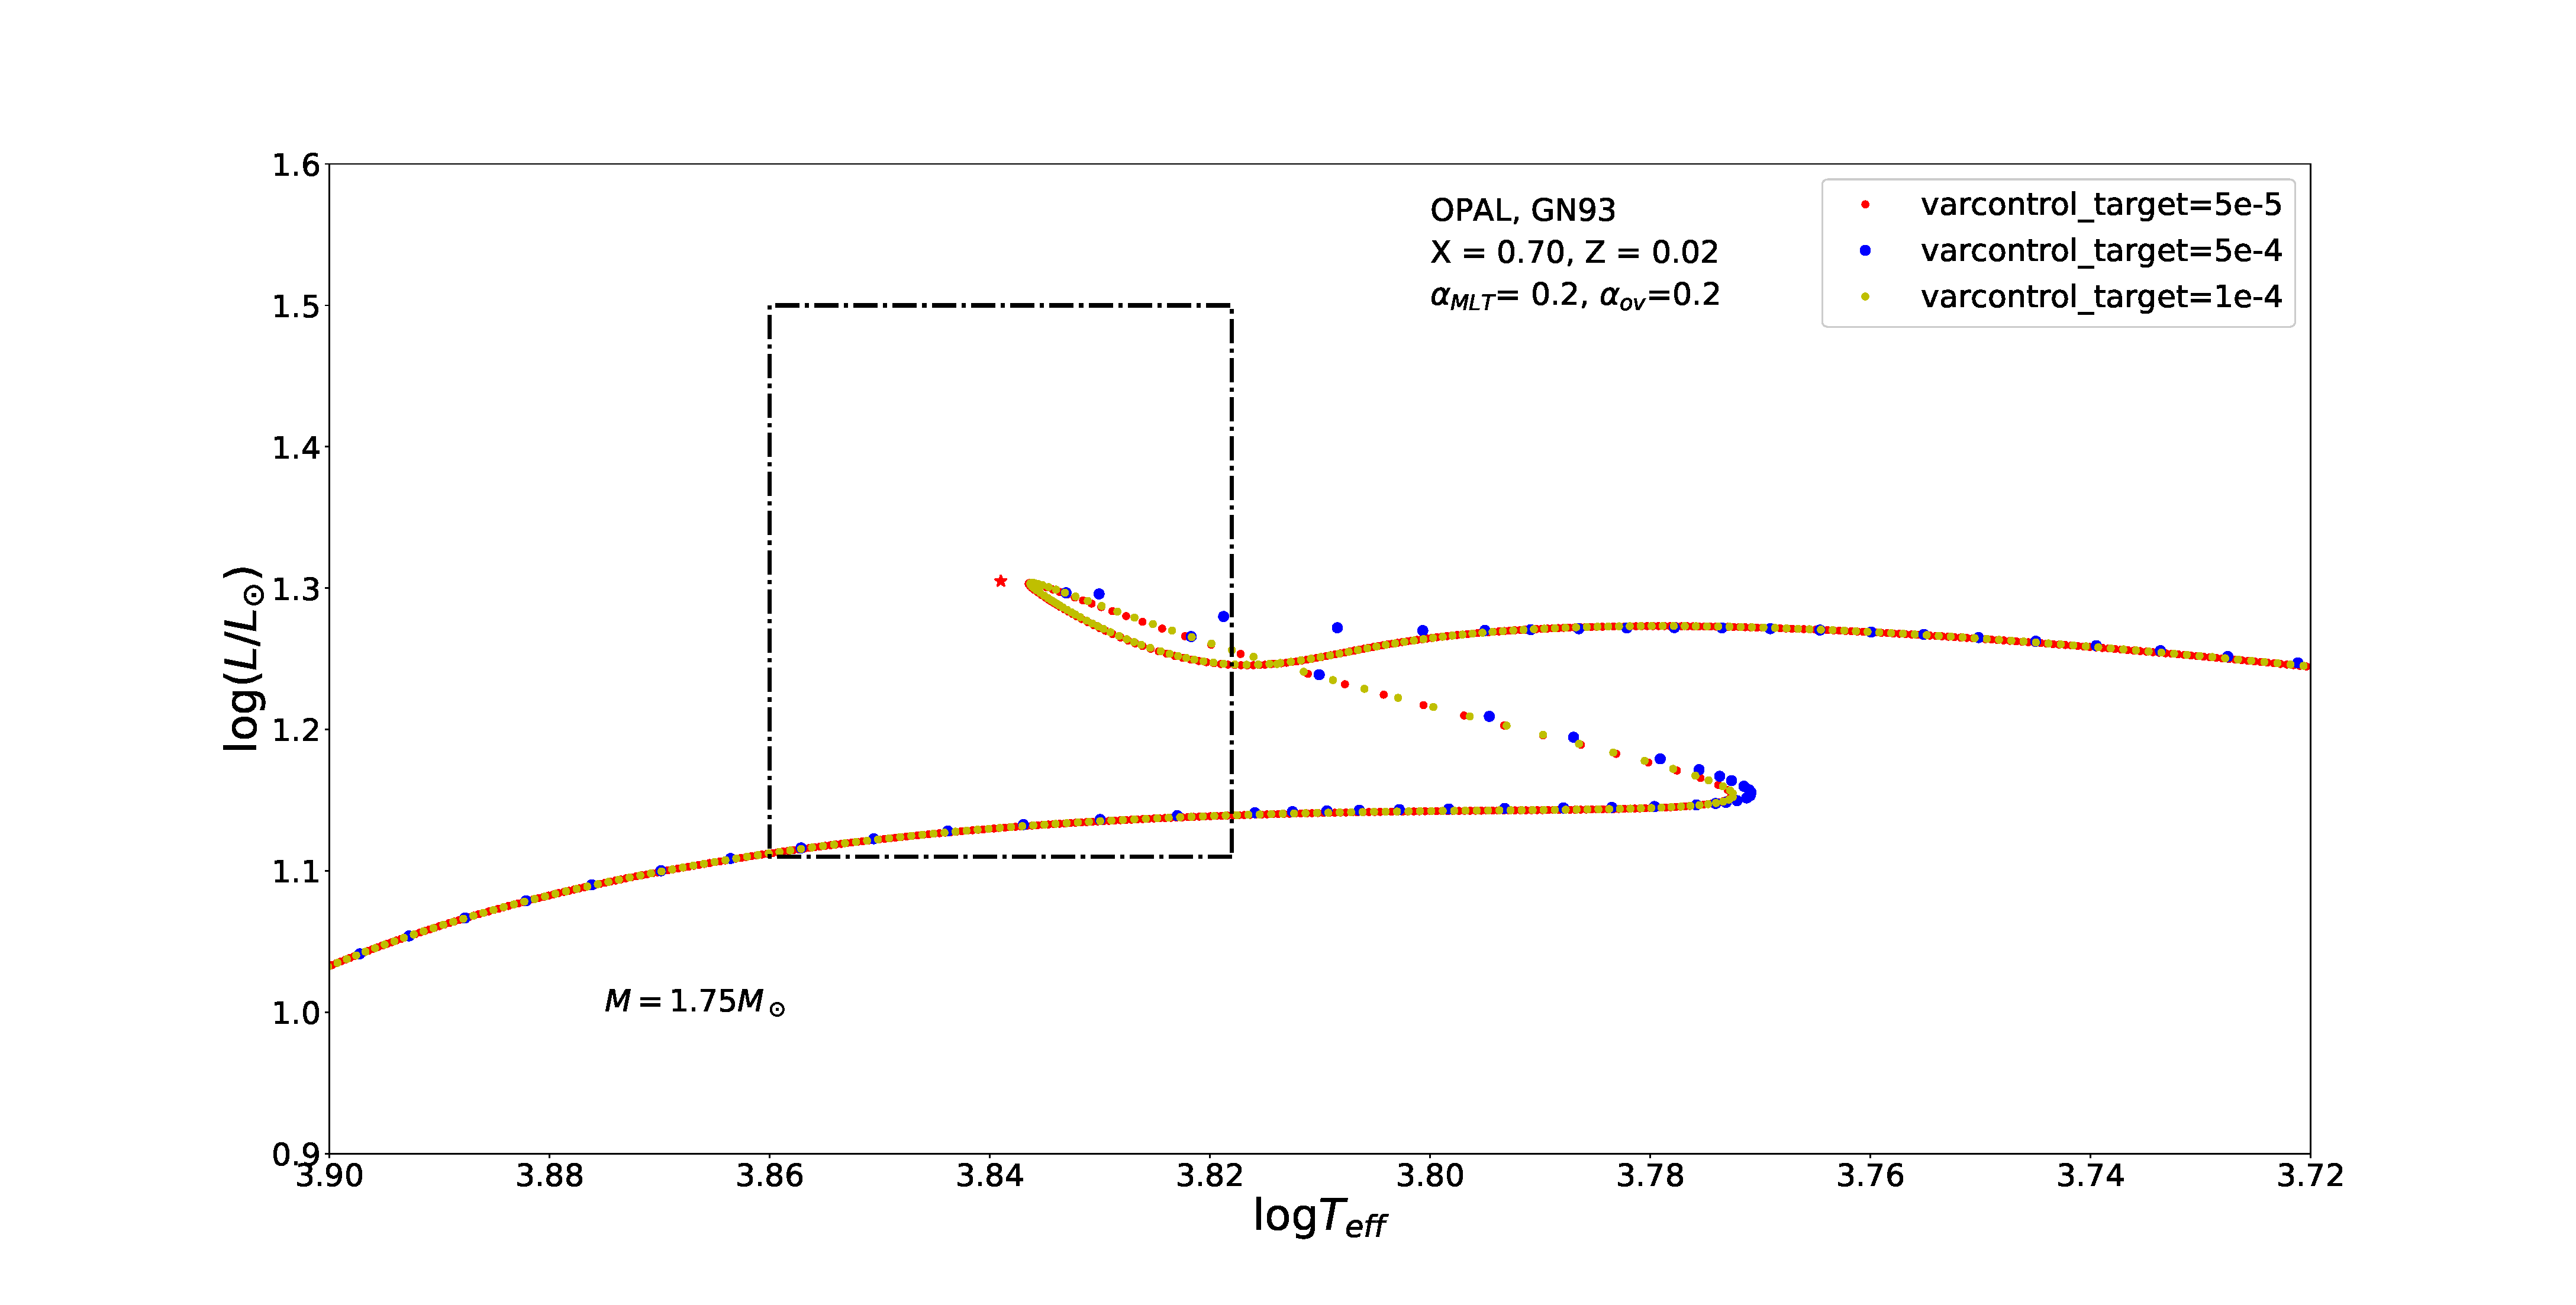
\includegraphics[width=1.2\textwidth]{varcontrol_res_2.eps}}%
    \caption{Evolution of three tracks with same initial parameters ($M= 1.75$\msun,$X=0.70, Z=0.02, \alpha_{mlt} = 0.2, \alpha_{ov} = 0.2$ ), but different values of \texttt{varcontrol\_target} where $1\cdot10^{-4}$ is default in \texttt{MESA}. It can be seen that the resolution drops significantly for the value $5\cdot10^{-4}$. Therefore, a slightly smaller value of $5\cdot10^{-5}$ is chosen for this work. Observational uncertainties from parameters from \citet{lenz2010delta} are marked as a black dashed errorbox. }
    \label{varcontrol}
\end{figure}


Some tracks are still better resolved than others. A general tendency from the computed tracks are that models with overshoot below 0.2 are not resolved nearly as well as models with high overshoot of 0.3, which can also be seen on \figref{ovresol}. Particularly the Henyey hook cannot be reproduced very well for overshoot of 0.1. The details as to why this occurs is beyond the scope of this work, however it is very important to take into consideration when evaluating results as tracks with low overshoot will automatically have fewer models and therefore limited chances of fitting well to observations. 

\begin{figure}[htbp]
    \centering
    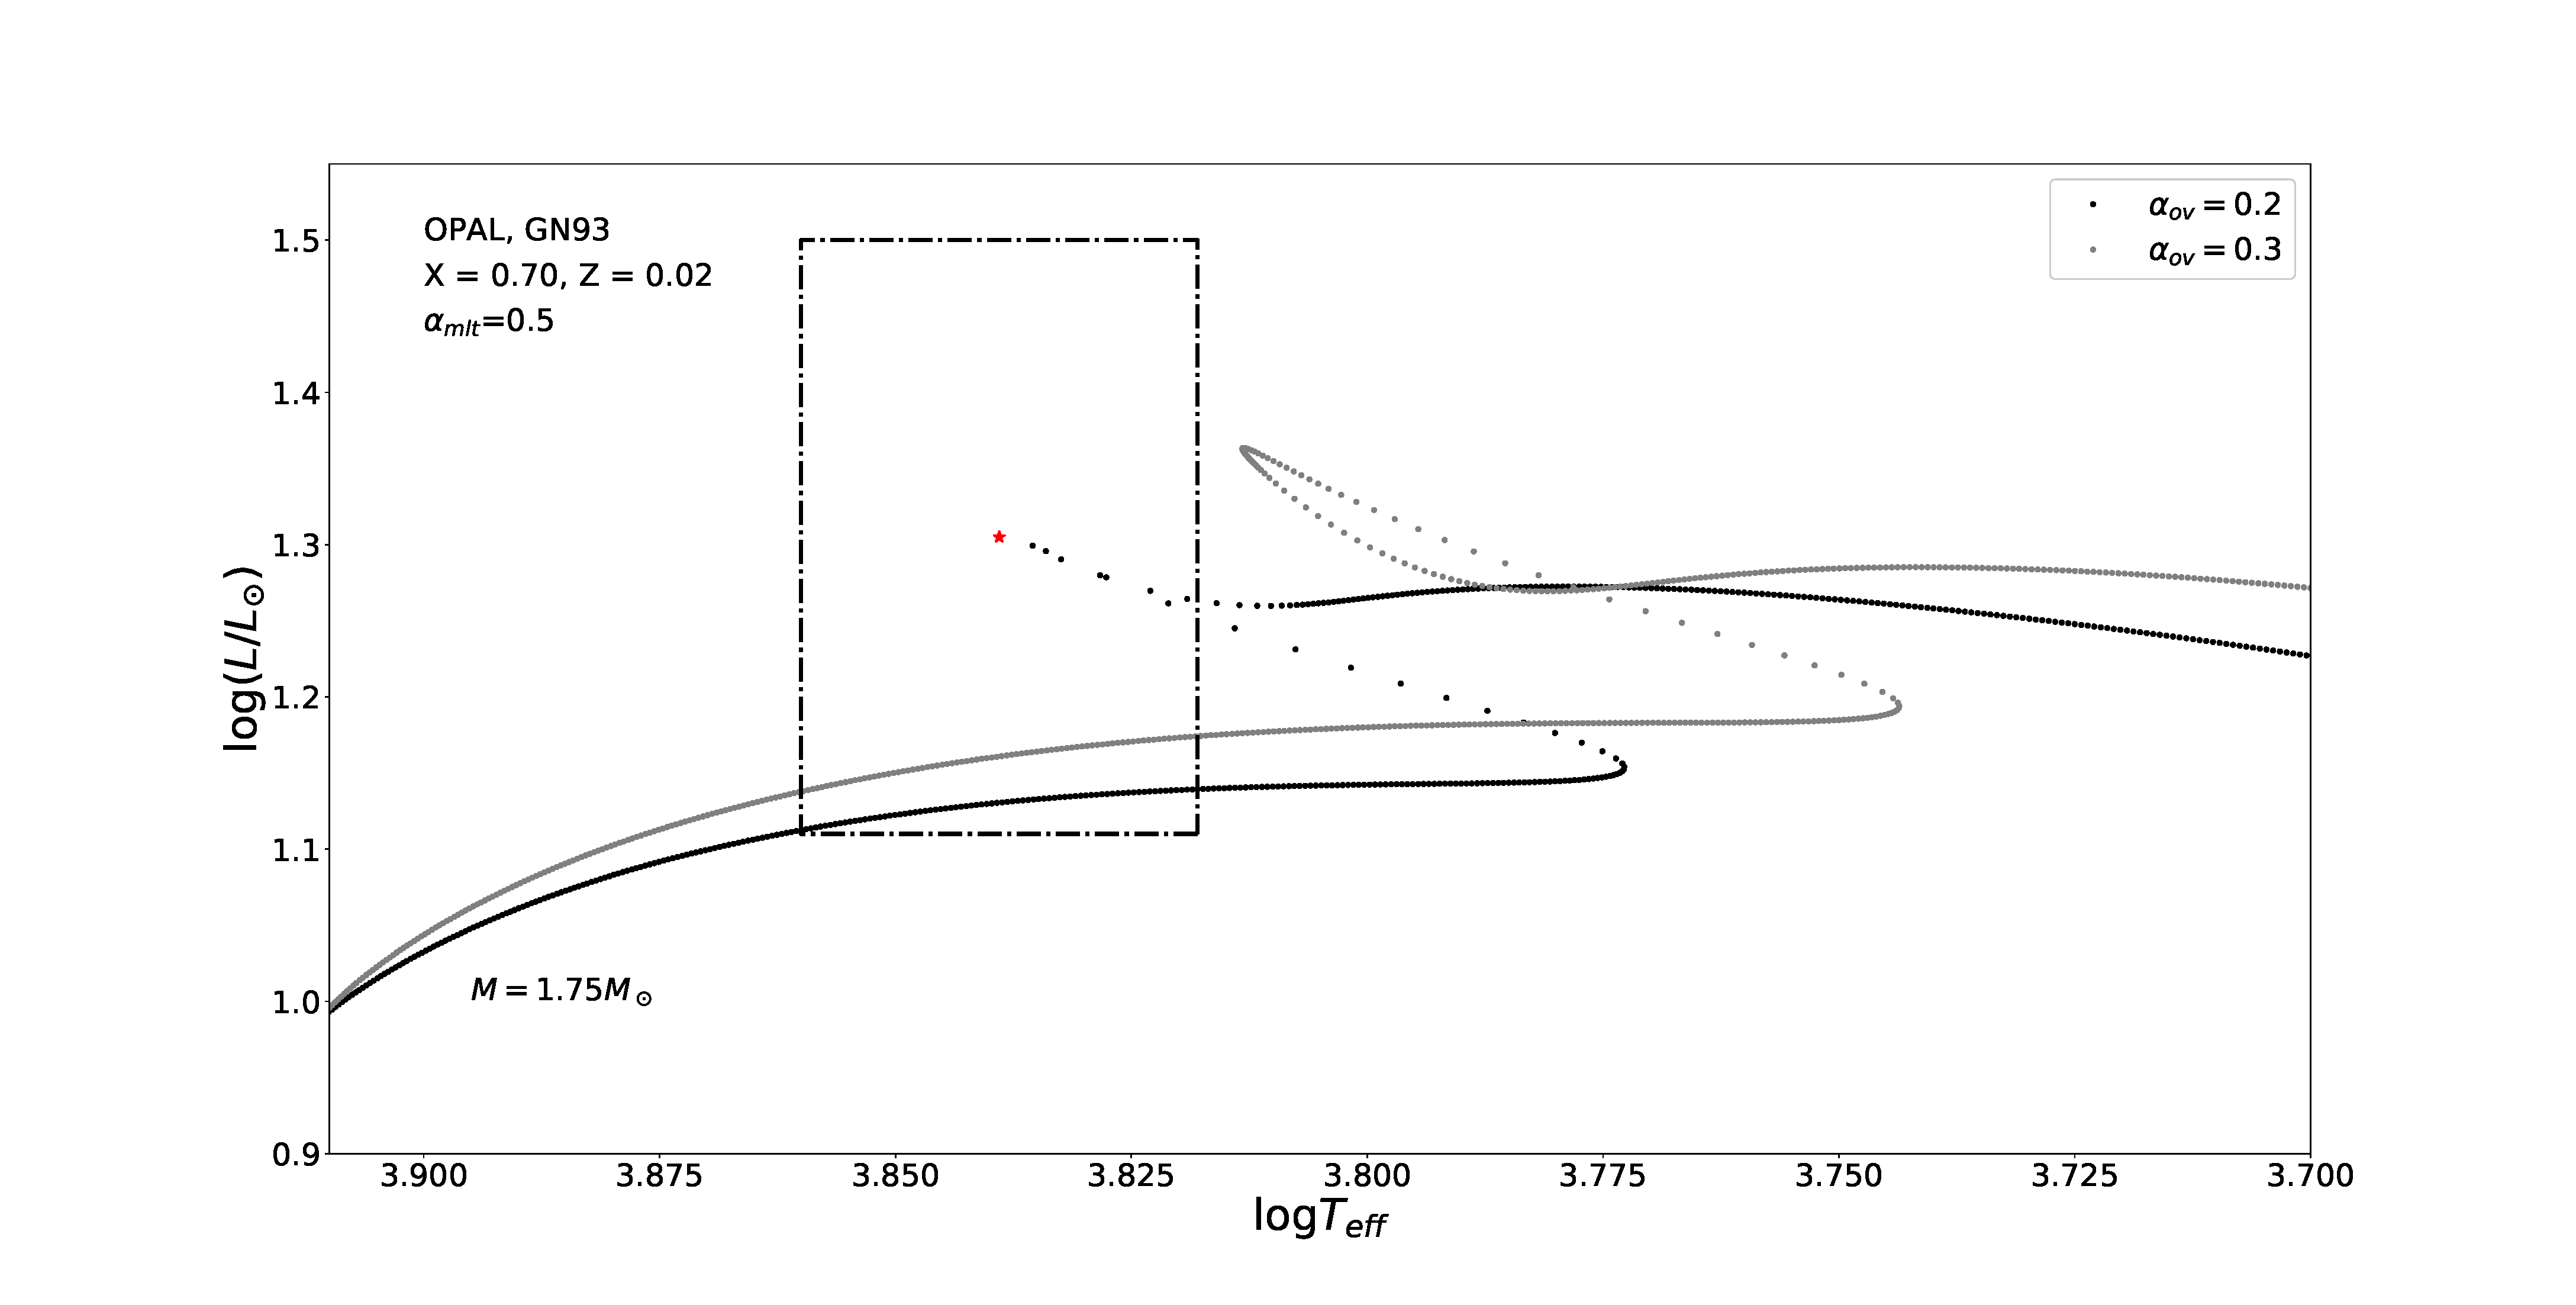
\includegraphics[width=1\textwidth]{resolution_overshoot.eps}
    \caption{Evolution of a track with two different overshoot parameters. $M= 1.75$\msun,$X=0.70, Z=0.02, \alpha_{mlt} = 0.5$.  Observational uncertainties from parameters from \citet{lenz2010delta} are marked as a black dashed errorbox.}
    \label{ovresol}
  \end{figure}


\section{$\chi^2$ testing}
\label{sec:chis}

\subsection{Finding the best model}
\label{bestmodel}


In order to find out how well a model fits the data, a comparison with stellar parameters is needed. By just comparing models to \lum,  \teff, and \logg, it is difficult to find an estimate on the evolutionary stage as the best model on one track might be on the main sequence, whereas the best model on a different track is on the post-main sequence. Therefore, frequencies are need as additional observational parameters for comparison (as they, as discussed in \secref{chap:asteroseismology}, change with evolution). There is more than one way of doing the comparisons, but in this work a \chis test is used. The \chis test yields a value for each model, allowing to find models with lowest \chis values. The Pearson's goodness of fit test is commonly written as 

\begin{align}
\label{standard_chi}
\chi^2_j = \sum^I_{i=1}\left(\frac{x^{\text{theo}}_{i,j}-x^{\text{obs}}_i}{\sigma_i}\right)^2,
\end{align}

\noindent where $x_i^{obs}$ is the observed parameter for the $i$'th fitting parameter (and $j$'th model), $x^{theo}_i$ is the corresponding theoretical parameter and $\sigma^i$ is the uncertainty of the $i$'th parameter. It provides a number that describes how close the fitting parameters are to the corresponding observed parameters. There are a few assumption that needs to be taken into consideration before implementing a \chis test. Most importantly, statistically speaking, a \chis test does not provide any information on how well individual parameters fit, or how likely a model is to be the best representative of the star. As the goal of this project is to estimate the evolutionary stage of the stars, the \chis values can simply be used as a way of \textit{comparing} between the different models. So models with the lowest \chis are the models with parameters closest to the observed parameters. 
If the \chis values are to be compared between the different models, then they need to be calculated under the same conditions. This means that calculations should be done with the same number of fitting parameters for all models (since they otherwise are not comparable). For instance, if one model have more fitted frequencies than another, the \chis of that model will have more fitting parameters, causing it to naturally be larger than the \chis for the model with fewer fitted frequencies, making their \chis incomparable. This will be taken into consideration in the routine described in \secref{highermodes}.

%GYRE produces an output file for the chosen MESA profiles. Since it computationally takes time to produce the output files, a constraint is needed in order to determine which profiles are within the range where we wish to produce a GYRE output file. This is done by defining a parameter space of size three sigma, based on observed parameters \teff, \lum, and \grav.

%In order to test how well the computed frequencies match observed frequencies a \chis prescription is applied to every profile. 
\subsection{44 Tau}
\label{sec:chi44}

\subsubsection{Radial modes}

For 44 Tau, the frequencies of the fundamental mode and first overtone are well-determined. These frequencies act as a constraint for the l=0 mode models. Initially the l=0 modes are computed using \texttt{GYRE} for the entire grid described in \secref{sec:grid}. Here, we have an initial constraint from only the frequencies corresponding to the radial fundamental mode, first overtone and the global parameters. The \chis for this initial run then becomes

\begin{align}
\chi^2_j & = & \left(\frac{\nu^{\text{fund,obs}}-\nu_j^{\text{fund,theo}}}{\sigma_{\text{fund},j}}\right)^2 
 + \left(\frac{\nu^{\text{first,obs}}-\nu_j^{\text{first,theo}}}{\sigma_{\text{first},j}}\right)^2 
 +
\left(\frac{\text{T}_\text{eff}^{obs}-\text{T}_{\text{eff},j}^{\text{theo}}}{\sigma_{\text{T}_\text{eff},j}}\right)^2 \nonumber \\
& & +
\left(\frac{\log \text{g}^\text{obs}-\log \text{g}^\text{theo}_j}{\sigma_{\log \text{g},j}}\right)^2 
 + \left(\frac{\log \text{L}^{\text{obs}}-\log \text{L}^\text{theo}_j}{\sigma_{\log \text{L},j}}\right)^2, 
 \label{eq:chis}
\end{align}

\noindent where $\chi^2_j$ is the \chis for the $j$'th model. For \teff, \logg and \lum, the $\sigma$ used are the uncertainties from observations. %Notice here that even though the frequencies are calculated for the entire track, the \chis is not calculated for models on the pre-MS. 

For the frequencies the $\sigma$ is naturally very small (in the order of $10^{-6}$), since the uncertainty on observations depend inversely on the observation time. Long observation times of 44 Tau therefore results in very narrow peaks. It is very nice to know a parameter to this precision, but as shown in \eqref{eq:chis} a small uncertainty will results in high values of \chis. High values of \chis are not an issue in itself, as they are simply numbers for comparison. It does however mean that the frequencies will naturally be weighted higher. The model precision is simply not comparable to frequency precision. In other words, no model will ever get close to fitting well. Also, by only dividing by the uncertainties the resolution of the track is not taken into consideration. As shown in \secref{sec:res} the resolution of the track is important as fewer models in the same range decreases the possibility of having a good fit within that space. This also means that a model frequency can change a lot between two time steps if the resolution is low, and this should be taken into account. In this work the following prescription is therefore applied to the frequencies: 
\begin{equation}
\label{sigma}
    \chi^2  = \sum^I_{i=1}\frac{\left(v^{\text{obs}}_{i}-v^{\text{theo}}_{i,j}\right)^2}{(\sigma^{\text{obs}}_i)^2 f_i(\Delta\nu_{i,j})}
\end{equation}

\noindent where $i$ in this case is the different frequencies (i.e I=2 for $l=0$ calculations where we only compare to fundamental frequency and first overtone) and $j$ is the $j$'th model. Lastly, $f_i(\Delta \nu_{i,j})$ is a function that artificially enhances the sigmas on the frequencies

\begin{equation}
\label{function}
    f_i(\Delta \nu_{i,j}) = \frac{\nu_j - \nu_{j-1}}{\sigma_{\text{obs},i}},
\end{equation}
 
\noindent where the distance in frequency space is taken into consideration for the j'th model. Smaller distances in the frequency space between model means a higher $f_i(\Delta \nu_{i,j})$, hence, as smaller \chis. Runs both with and without the uncertainty pump will be made to test the difference in the main result. 

%Alternatively, the \chis for the frequencies can be calculated as \eqref{standard_chi}, but with an expanded $\sigma$ similar to that of a standard deviation

%\begin{equation}
%\label{m2}
   % \sigma_{i,j} = \frac{1}{I}\sqrt{\sum_{i=1}^I \left(\nu_{i,j}^{\text{theo}} - \nu_{i}^{\text{obs}}\right)^2}.
%\end{equation}

%There are both advantages and disadvantages for both methods. The first method does take the spacing into consideration, but it follows from this that the since the \chis are artificially enhanced, the scaling between the frequency \chis and rest of the parameters is off by the scaling factor $\alpha$. This can be found by finding the ratio $\frac{\chi_{freqs}}{\chi_{freqs}}$ for each model, j, and finding the mean. This method is slightly more complicated than the second method, however, the second method does not take the spacing in frequency between models into account, and the standard deviation is based only on two different frequencies. The order of magnitude of the \chis is different for the methods, but as mentioned earlier the numbers themselves are not representative of how well a model fits. 

As of yet only l=0 modes have been fitted. Calculating corresponding l=1 and l=2 modes for all models is time consuming, and therefore a selection criteria is needed. This is done by first finding the model with the lowest \chis is for each track. From all of these the best 5\% are found for both observational parameter sets as listed in \tabref{obsparams}. These models and their input parameters are shown in \tabref{bestchi_m1}. The difference between the different runts can be seen in the last column.  

%\begin{center}[htbp]
\begin{longtable}{ccccccc} 
\caption{List of models that are within the 5\% lowest \chis values for 44 Tau. } \label{bestchi_m1} \\
\toprule
Model &  $M[M_\odot]$ &X & Z & $\alpha_{mlt}$ & $\alpha_{ov}$ & Parameter set\\  
\midrule
1238 & 1.50 &0.65  & 0.01 & 0.2  & 0.3 & 1,2\\
1201 & 1.50&0.65 & 0.01 & 0.5 &  0.1   & 1,2\\
1211 &  1.50 &0.65& 0.01 & 0.5 &  0.3  & 1,2 \\
1214& 1.50 &0.65 &  0.01& 0.8 &  0.2  & 1,2 \\
1168 &  1.50&0.65&  0.01& 0.8 &  0.3  & 1,2\\
1190 & 1.55 &0.65&  0.01& 0.2 &   0.2  & 1,2\\
1411 &  1.60 &0.70&  0.01& 0.2 &  0.3 & 1,2 \\
1434& 1.60 &0.70&  0.01& 0.5 &   0.3  & 1,2\\
1244 & 1.60 &0.70&  0.01& 0.8 & 0.3   & 1,2\\
1353& 1.60 &0.70&  0.01& 0.8 &  0.3    & 1,2 \\
1204& 1.60 & 0.70& 0.01 & 0.5 & 0.1  & 1,2\\
1264 & 1.60 &0.70& 0.01 & 0.8 &  0.1 & 1,2 \\
1384& 1.65 &0.70& 0.01 &  0.2&   0.2  & 1,2\\
1428& 1.65 &0.70&  0.01 & 0.5 &  0.2  & 1,2\\
1328& 1.65 &0.70&  0.01& 0.2 &  0.2  & 1,2\\
1289 & 1.65 &0.70&  0.01& 0.2 &  0.3 & 1,2\\
1353&  1.701& 0.65& 0.02 & 0.2 &  0.1  & 2 \\
1144&  1.701 & 0.65  & 0.02  & 0.5 & 0.2   & 1,2  \\
1121&  1.701 & 0.65  & 0.02  & 0.8 & 0.1   & 2  \\
1131 &  1.701 & 0.65  & 0.02  & 0.8 & 0.2   & 2  \\
1140&  1.701& 0.75& 0.01 & 0.8 &  0.3  & 1 \\
1290&  1.701& 0.75& 0.01 & 0.5 &  0.3  & 2 \\
1148&  1.701& 0.75& 0.01 & 0.8 &  0.2  & 2 \\
1126&  1.701 & 0.65 & 0.02 &  0.8&  0.1 & 1\\
1273&  1.75 & 0.75 & 0.01 &  0.2& 0.2   & 1,2 \\
1187&  1.75 &  0.75 & 0.01 &  0.5 &  0.2  & 1,2\\
1216&  1.75 &  0.65 &0.02&   0.2&  0.2  & 1\\
1231&  1.75 &  0.65 & 0.02 &  0.2&   0.3 & 1,2\\
1158&  1.75 &  0.65 & 0.02 &  0.5  & 0.3 & 1,2 \\
1177&  1.80&  0.70 &  0.02&  0.2  &   0.2 & 1,2 \\
1165&  1.80&  0.70 & 0.02 &   0.5 &  0.3 & 1,2 \\
1271&  1.85&  0.70 & 0.02 &  0.2 & 0.2   & 1,2 \\
1089&  1.85& 0.70&  0.02 &  0.5 &   0.2  & 1,2\\
1065&  1.85& 0.70 &  0.02& 0.8  &  0.2  & 1,2\\
1137&  1.85&  0.65&  0.03 &  0.2  & 0.1  & 1,2\\
1230&  1.85&  0.65& 0.03 &  0.2  & 0.3 & 1\\
1025&  1.85 &  0.65& 0.03 &  0.8 &  0.2 & 1,2 \\
1219& 1.90 & 0.70&  0.02&  0.2&  0.3  & 1,2\\
1074&  1.90&  0.70& 0.02 &  0.5&  0.2  & 1,2\\
1071&  1.90 &  0.70&  0.02&  0.8&  0.2  & 1,2\\
1086&  1.95 &  0.75&  0.02&  0.5& 0.1 & 1 \\
1072&  1.95 &  0.75&  0.02&  0.8& 0.1 & 1,2\\
1023&  1.95 &  0.70& 0.03& 0.8  & 0.2 & 1,2\\
1088&  2.0&  0.75&  0.02 &  0.5  & 0.1 & 1,2\\
1069&  2.0&  0.75&  0.02&  0.5  & 0.2 & 1,2\\
1050&  2.0&  0.75&  0.02&  0.8  & 0.1 & 1,2\\
1046&  2.0 & 0.75 & 0.02 &  0.8  & 0.2  & 1,2\\
1123&  2.0 &  0.70&  0.03&  0.2  & 0.2 & 1,2\\
1030&  2.0 &  0.70&  0.03& 0.5  & 0.1 & 1,2\\
1010&  2.0&  0.70&  0.03& 0.8  & 0.1 & 1,2\\
1151&  2.05& 0.75 & 0.02 &  0.2& 0.1 & 1,2\\
1129&  2.05&  0.70& 0.03 & 0.2 & 0.1 & 1,2\\
994&  2.05&  0.70&  0.03&  0.8  &0.2 & 1,2\\
1156&  2.10&  0.75&  0.02&  0.2  & 0.2 & 1,2\\
1073&  2.10&  0.75&  0.02&  0.8  & 0. 3& 1,2\\
1090& 2.10 &  0.70&  0.03&  0.5& 0.3 & 1,2\\
1010 & 2.15 &  0.75 &  0.03 & 0.5  & 0.2 & 1,2\\
1219&  2.20&  0.75&  0.03&  0.2  & 0.3  & 1,2\\
1055&  2.20&  0.75& 0.03 &  0.5  & 0.1 & 1,2\\
1087&  2.20& 0.75 &  0.03&  0.5  & 0.3 & 1,2\\
1034&  2.20& 0.75 &  0.03&  0.8  &0. & 1,2\\
979 &  2.20&  0.75 &  0.03& 0.8  & 0.2 & 1,2\\
1068&  2.20& 0.75 & 0.03  & 0.8   & 0.3 & 1,2\\ \bottomrule
\end{longtable}
%\end{center}

 By first selecting the model with the lowest \chis value for each track, a wide range of parameter combinations is ensured. It forces an estimate on the evolutionary stage at all areas of the grid, including the very outskirts. The disadvantage of this is that it makes it more difficult to identify the most likely parameter combination, since there cannot be more than one model in the 5\% range on a track. However, as the end goal is to find an estimated evolutionary stage and a single best model, the method is adequate.

%The selection of the 5\% best models is illustrated on \textbf{LAV REFERENCE}
%and \textbf{LAV REFERENCE} for the two different luminosities and methods respectively. Upper panels shows models with \chis calculated from \eqref{sigma} and lower panels \eqref{m2}. The \chis are plotted as a function of mass. The red line represents the 5\% line, where models below the lines are marked with red, meaning that they are amongst the 5\% models with the lowest \chis value. The different method does show slight differences in the distribution of \chis values. However, what can be seen on all the plots is that the spread in the \chis values is higher for the outskirt values of the mass, particularly towards the lower end, whereas models with a mass of 1.95\msun generally have lower \chis values. This indicates that a mass of 1.95\msun leaves more room to change the rest of the parameters without changing the \chis significantly, including the frequencies. However, a mass of 1.5\msun have a significantly smaller range where it matches the observed parameters.

% \begin{figure}
%      \centering
%      \begin{subfigure}[b]{0.3\textwidth}
%          \centering
%          \includegraphics[width=\textwidth]{graph1}
%          \caption{$y=x$}
%          \label{fig:y equals x}
%      \end{subfigure}
%      \hfill
%      \begin{subfigure}[b]{0.3\textwidth}
%          \centering
%          \includegraphics[width=\textwidth]{graph2}
%          \caption{$y=3sinx$}
%          \label{fig:three sin x}
%      \end{subfigure}
%         \label{5pl1}
% \end{figure}

% \begin{figure}
%      \centering
%      \begin{subfigure}[b]{0.3\textwidth}
%          \centering
%          \includegraphics[width=\textwidth]{graph1}
%          \caption{$y=x$}
%          \label{}
%      \end{subfigure}
%      \hfill
%      \begin{subfigure}[b]{0.3\textwidth}
%          \centering
%          \includegraphics[width=\textwidth]{graph2}
%          \caption{$y=3sinx$}
%          \label{}
%      \end{subfigure}
%         \label{5pl2}
% \end{figure}

Since \chis only provide a value to compare to other models, it does not give an indication of how likely a
parameter space is. This also means that the \chis for the frequency space can deviate a lot from the \chis from the other observable parameters. To ensure that the 5\% models are also within the observable parameter space of \logg and \teff, a scatter plot is made which can be seen on \figref{scatter}. 

\begin{figure}[htbp]
	\centering
	%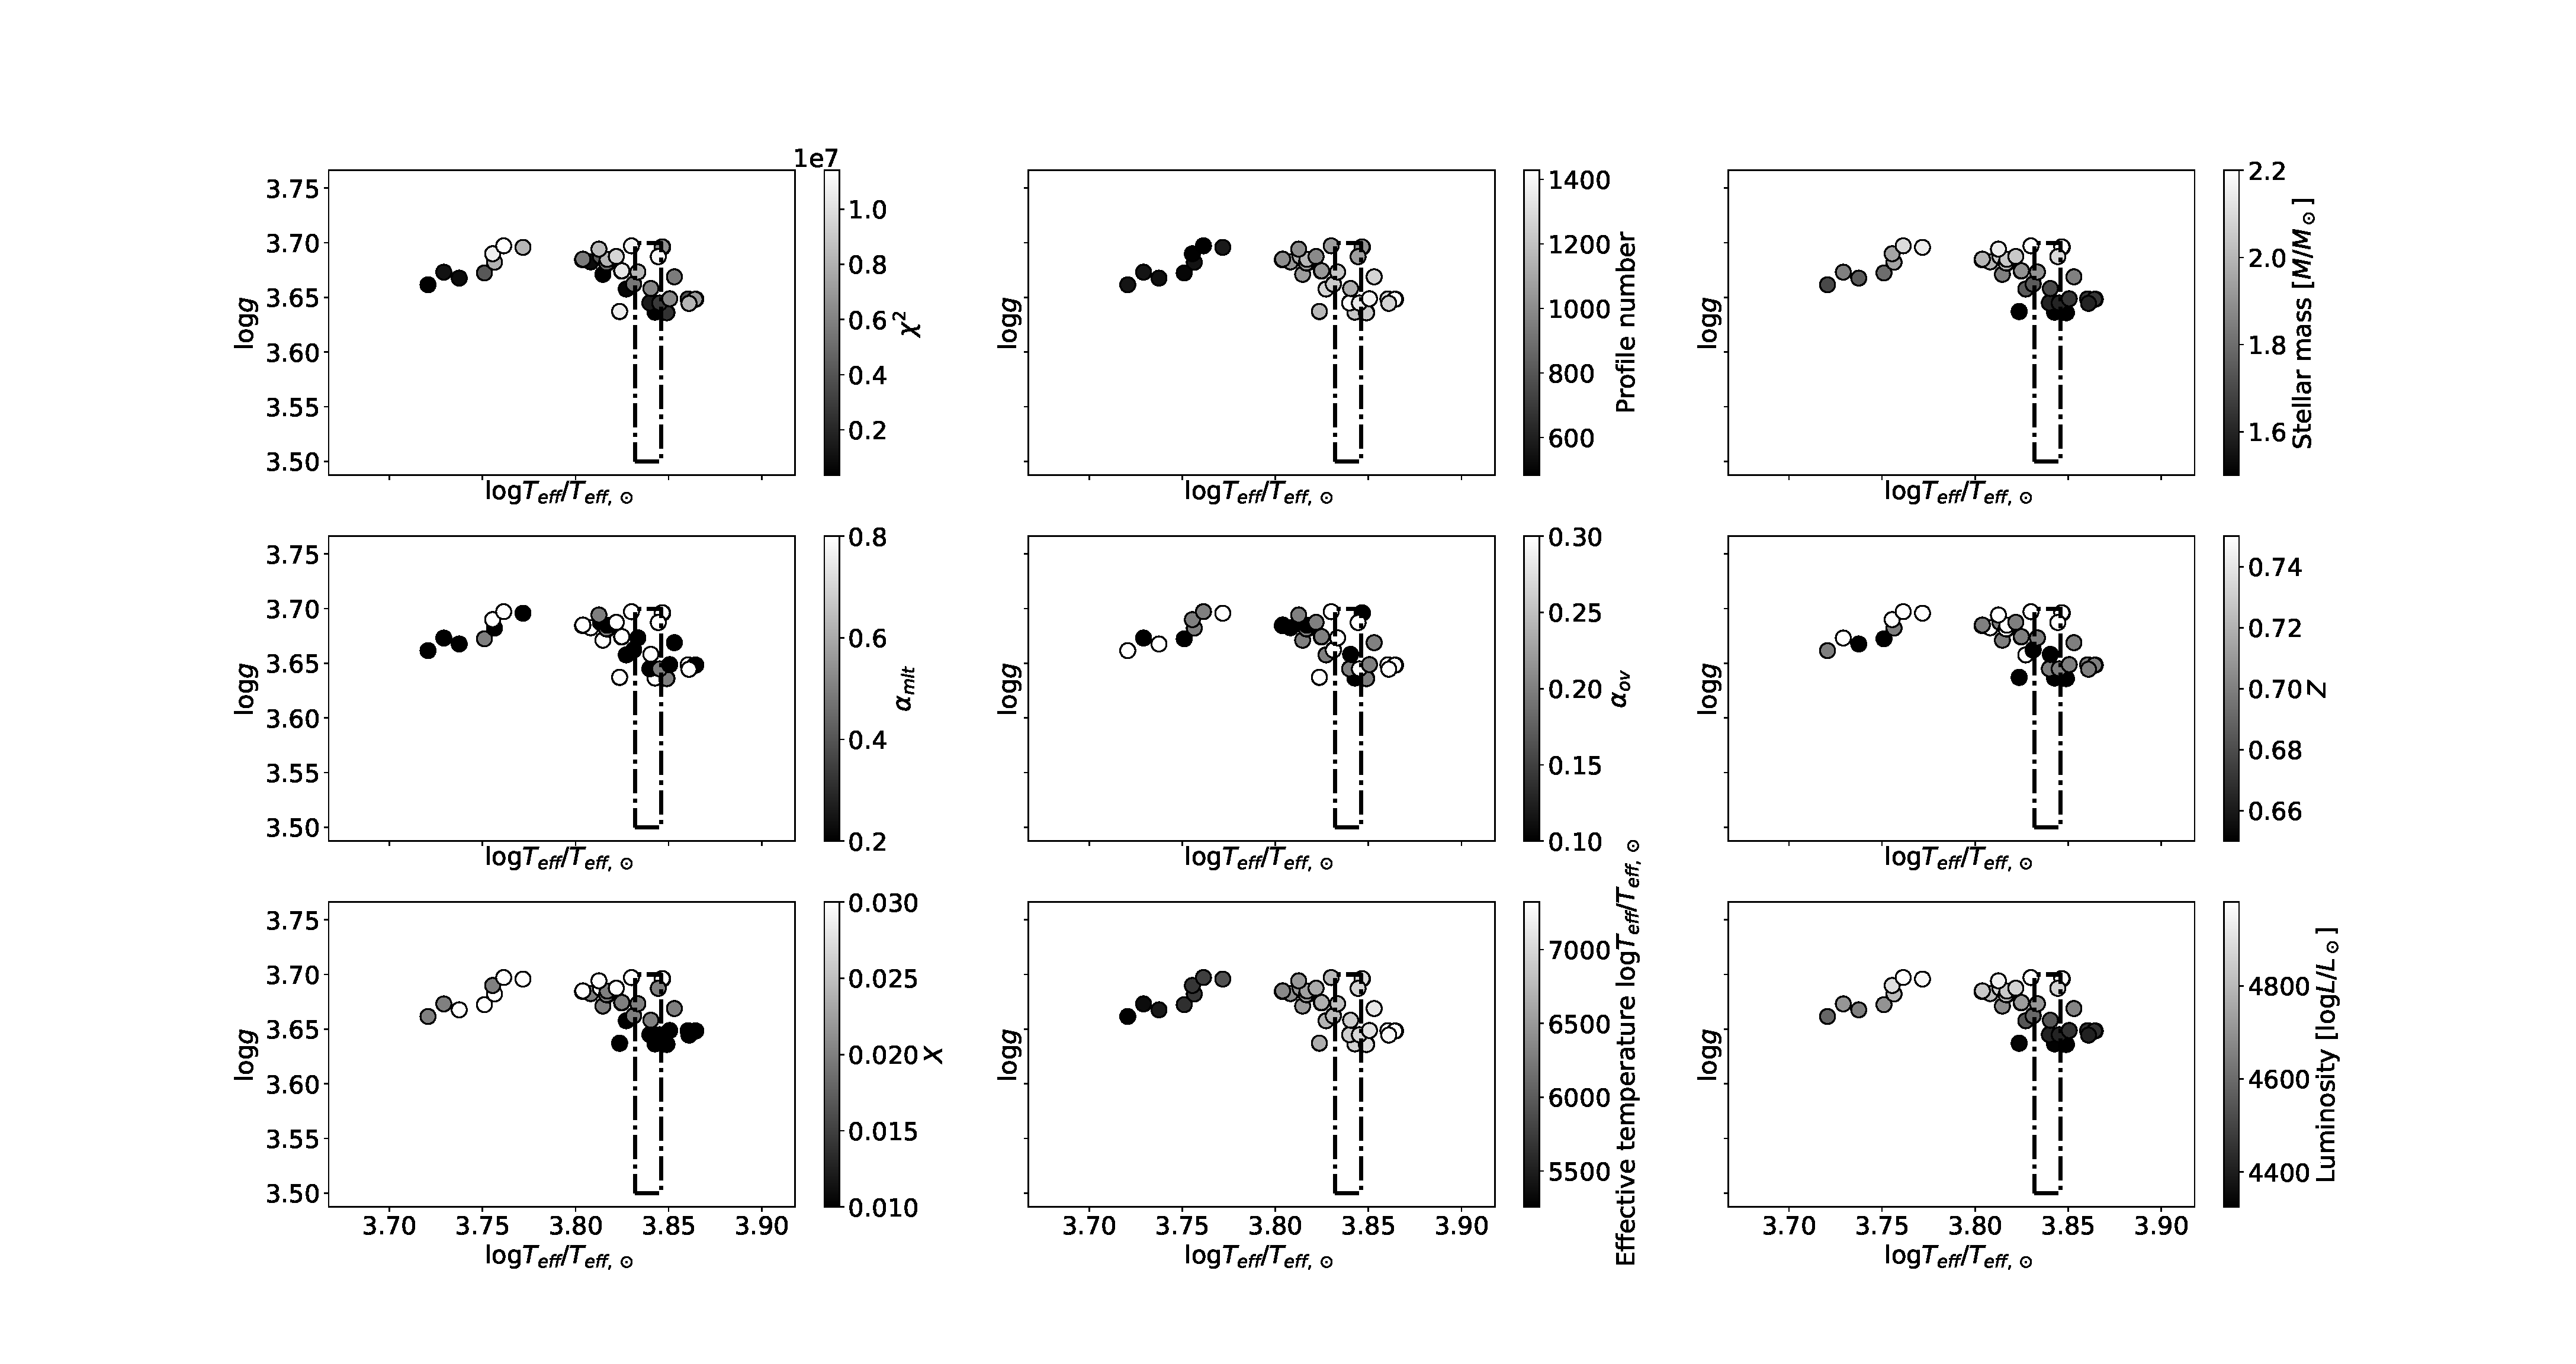
\includegraphics[width=1\textwidth]{scatter_all_v2.eps}
	\makebox[\textwidth][c]{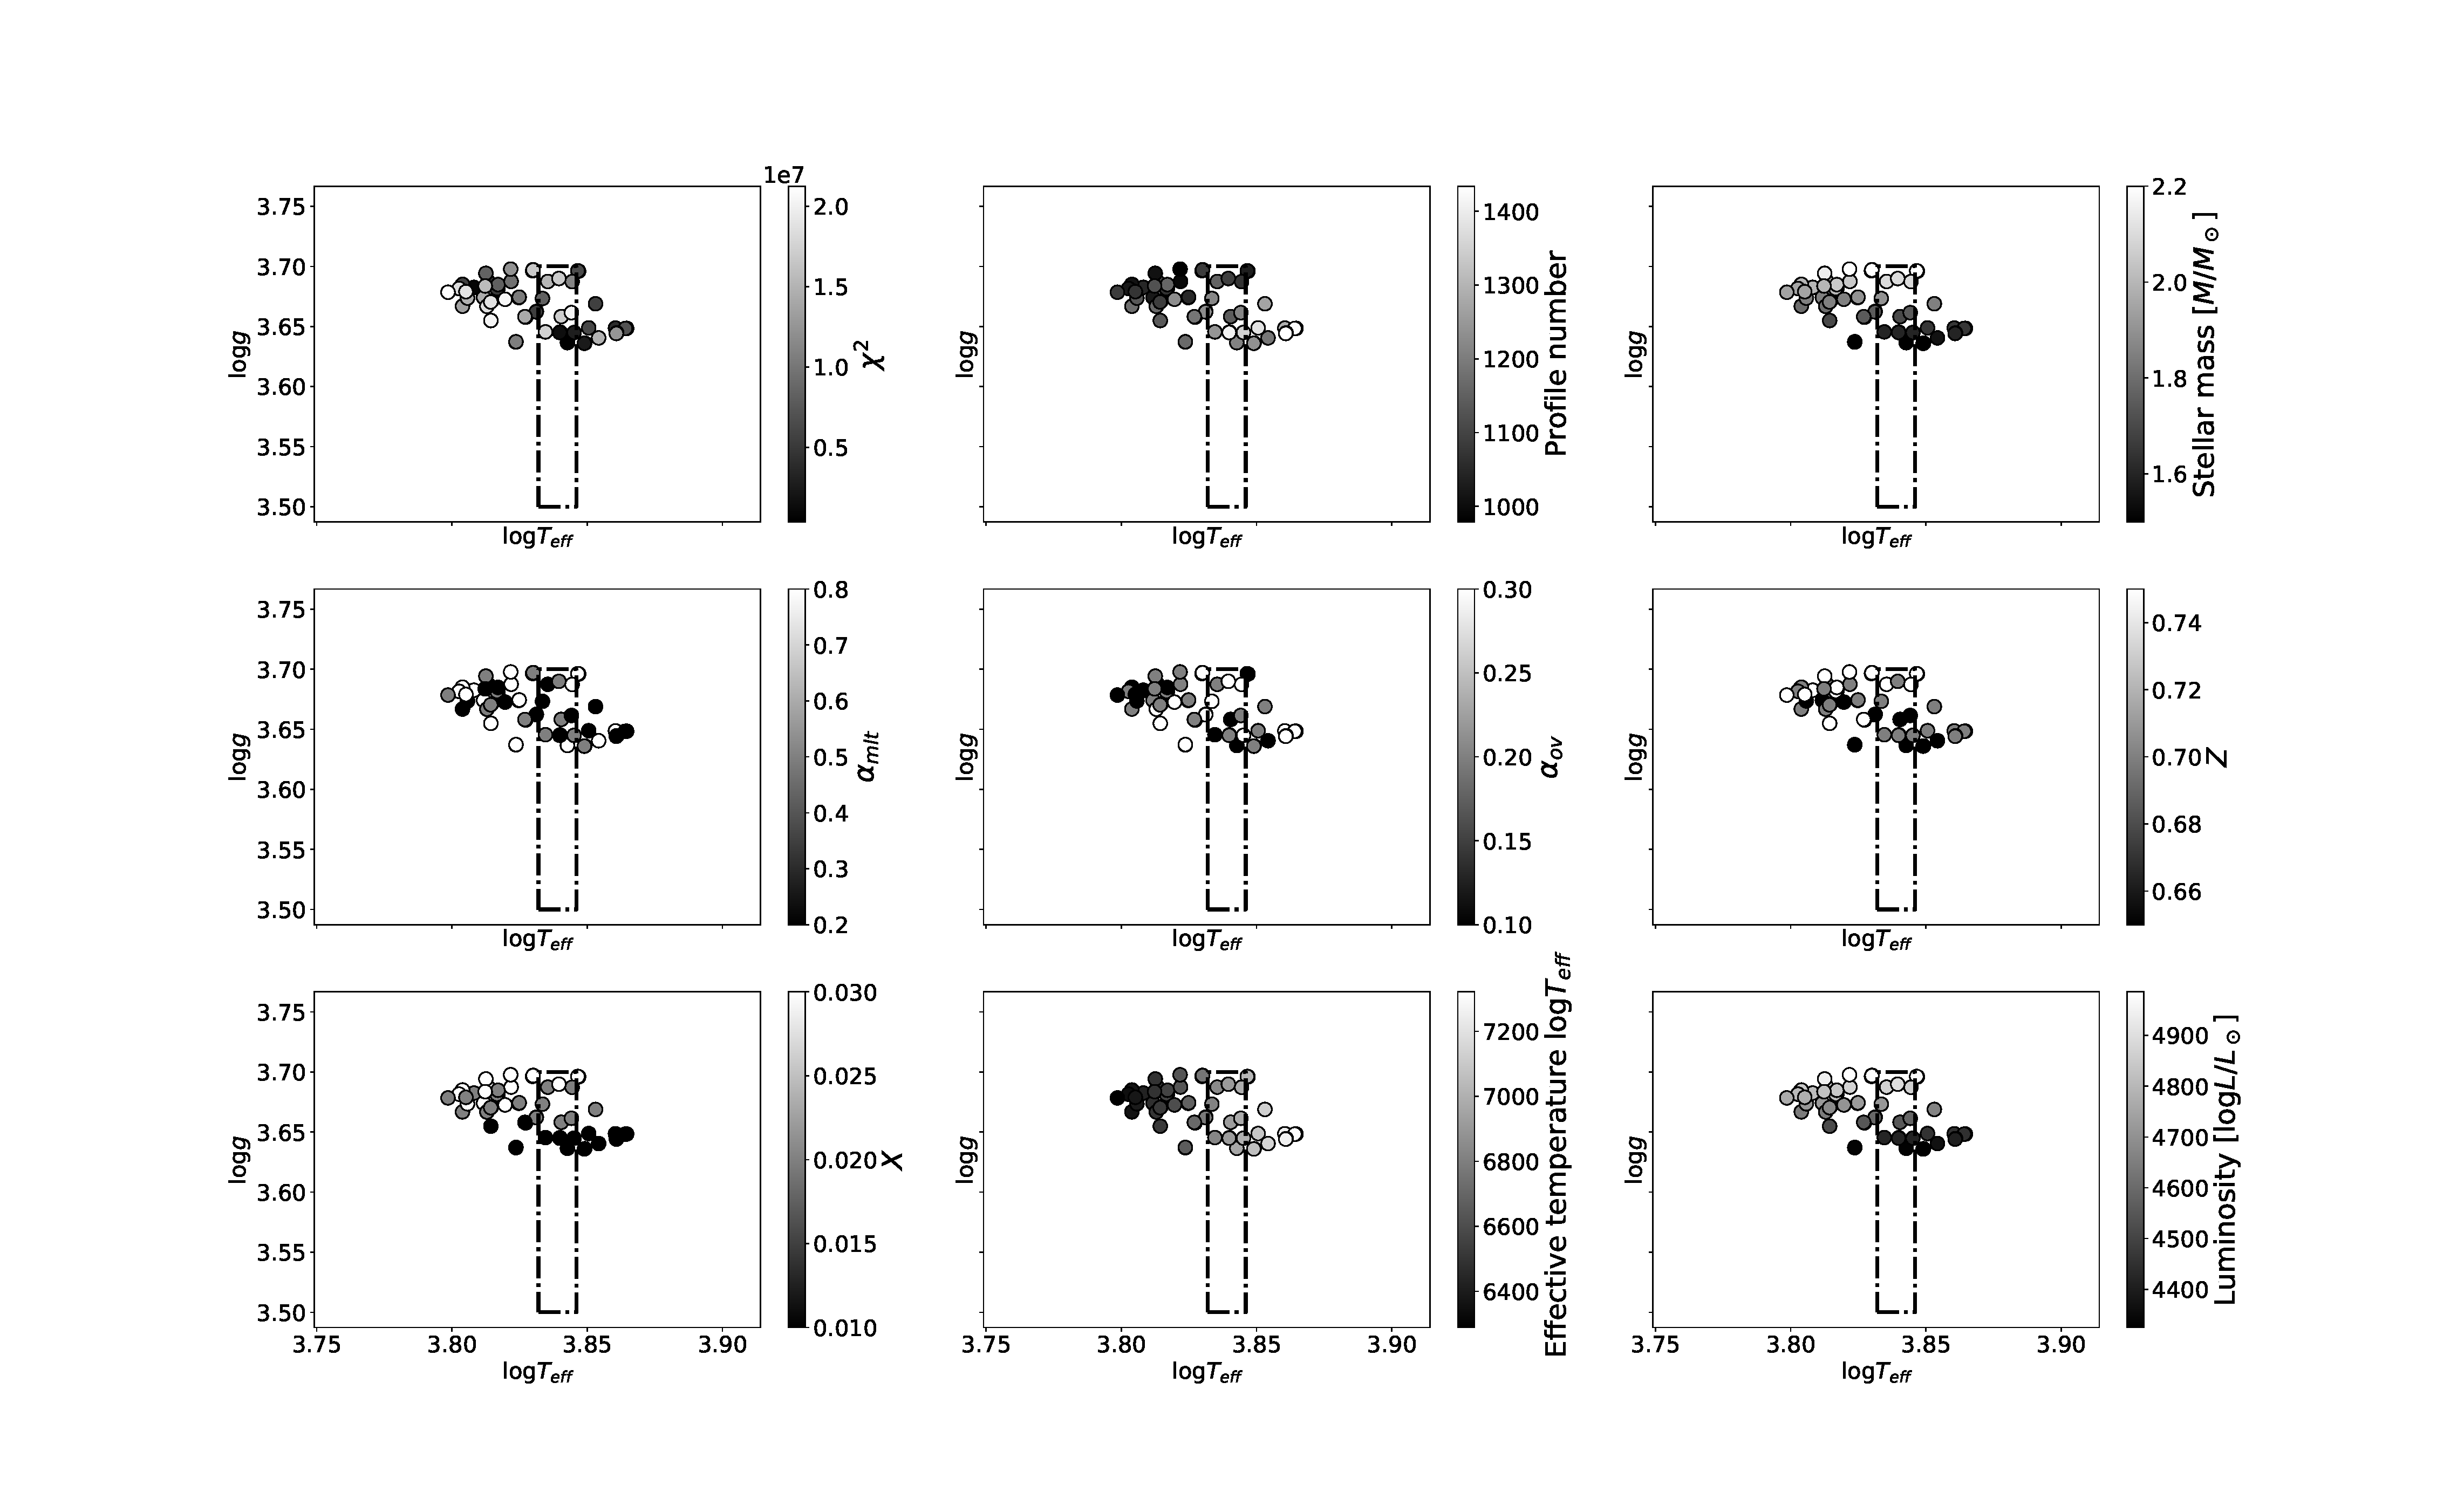
\includegraphics[width=1.5\textwidth]{scatter_final.eps}}%
	\caption{Scatter plots showing \teff, \logg color coded with nine different parameters for the 5\% best models (without resolution control). The plots color coded with \teff and \logg are plotted to show that the plotting method works correctly. The run was made with the Lenz obsevational parameters set. }
	\label{scatter}
\end{figure}


Here, \logg is plotted as a function of \teff and color coded with the corresponding \chis. The 1$\sigma$ uncertainty on \logg and \teff is marked with a black stippled line. Some of the scatter plots shows expected tendencies such as \lum, \logg, \teff and profile numbers. Since higher profile number is at a later stage\footnote{Note that the profile number does only indicate the stage of that individual track i.e profile number 900 on one tracks is not necessarily at the same stage for the same profile number on a different track. }, the effective temperature is much lower for lower profile numbers.%There is a gap in models around \teff = 3.79 in the 5\% selection criteria. From the profile number it is also clear that the models distributes into two groups where the lower profile numbers corresponds to those on the pre-ms and the higher profile numbers are ms and thereafter. The pre-ms models will be ignored since they are not as reliable as the rest of the models. This group of models is also significantly further away from the errorbox and they will therefore not affect the main result. 

The lowest \chis seems to linearly decrease with \teff. This is because \logg is strongly related to $\rho$ (hence, $\Delta \nu$ and \teff).  For the element abundances, there is a trend a that lower values of \logg yield lower values of Z and X, in particular. This falls out of \eqref{meanmol} as high abundances of hydrogen and/or metallicity causes a lower mean molecular weight $\mu$. Since $\mu \propto \rho \propto g$, a smaller value of X or Z yields a smaller value for g as well. Since $g$ is also directly proportional to the mass, the mass decreases with \logg in the plot as well. 

There seems to be no recognizable trend in the $\alpha_{mlt}$ and $\alpha_{ov}$ color coding. Since there is a definite correlation between the convection and structure of the star, it would be expected to see a trend between the mixing length or overshoot parameter and \logg and \teff. Since this sample is small, it cannot be excluded that there is a trend that can be found if more data points are included.   


\subsubsection{Nonradial modes}
\label{highermodes}
A new calculation is conducted in \texttt{GYRE} for $l=0,1,2$ modes for all of the 5\% models. The frequencies produced gives a further constrain of the best models as all frequencies can now be compared with observations. 

Calculations of \chis are conducted based on the fact that $n$ and $l$ is known for the models, but does not include a comparison to $l$ of the observed models. To ensure that the \chis are comparable between each model, as mentioned earlier, the models all need to have the same amount of fitting parameters. This is not an issue in the initial \chis calculations with $l$=0, since this \chis is only based on the same two frequencies for all models. But including $l=1$ in the calculations require that all observed frequencies are fitted to a corresponding theoretical match (so if the number of theoretically produced frequencies is lower than the observed, the model will be excluded).

It is carried out in the following way: for each model, each individual model-frequency is compared to all observed frequencies and the best match (i.e. the smallest difference) is thereby assumed to be the closest frequency. This is repeated from the lowest to highest frequency until all model-frequencies have been given a best match observation frequency. This means that the observed frequency will be given the $n$ and $l$ of the best matching model frequency. Each model then has an estimated set of frequencies where \chis can be computed. It does not take into consideration that the radial fundamental mode and first overtone are already determined (and might match it to n that are higher, however these models should be excluded as their match will not be good if the two first frequencies do not match expectations). This yields


\begin{align}
\chi^2 &= \left(\frac{\nu_{\text{all,obs}}^i-\nu^i_{\text{all,theo}}}{\sigma^i_{\text{first}}}\right)^2
 +
         \left(\frac{\text{T}_\text{eff,obs}^i-\text{T}_\text{eff,theo}^i}{\sigma^i_{\text{T}_\text{eff}}}\right)^2  \nonumber \\
  & \quad +
\left(\frac{\log \text{g}_\text{obs}^i-\log \text{g}_\text{theo}^i}{\sigma^i_{\log \text{g}}}\right)^2  + \left(\frac{\log \text{L}_\text{obs}^i-\log \text{L}_\text{theo}^i}{\sigma^i_{\log \text{L}}}\right)^2.
 \label{eq:chis_all}
\end{align}

From these, the models with the lowest \chis is found for the two different luminosities respectively.

As mentioned, this routine does not take the identified $l$ into account. The first way to do so is to weight each frequency individually by including a comparison between theoretically produced $l$ and the one from mode identification. Though this method probably provides a more detailed and statistically stringent result, it is does require a thorough estimate and evaluation of the single frequencies, which is beyond the scope of this work.
% and instead it is therefore made sure in the way the code is constructed, that this can only be an issue if the number of theoretically produced frequencies is lower than the observed number 8and this is unlikely to happen as these models have already been sorted out in the first \chis round. 


\subsection{Results}
The best models found for the two different runs of 44 Tau are shown in \tabref{bestmodels} and \tabref{bestmodels_continued}. The variation from parameter set 1 and parameter set 2 does not affect the total result, as the $\chi_{tot}$ does not differ down until a factor $10^{-13}$. It does however shift the best found model if only including the observational parameters. The reason for this is that the frequencies weigh more in the \chis than the observational parameters. Artificially enhancing the frequencies does shift the model to a higher mass (closer to the mass estimated by \citet{lenz2010delta}), but the $\chi_{ tot}^2$ is higher for this model. Enhancing the uncertainties corresponds to adding a weight to the frequencies. However, the difference between the weighted and unweighted results is of order 1, not changing overall result that frequencies still dominates the final outcome. 


\begin{sidewaystable}
	\caption{Best models for the two different observed parameter sets for 44 Tau. The two different parameter sets yielded the same overall result for best model. The difference in the \chis between the two parameter sets is0 insignificant (in the order of $10\cdot^{-13}$ except for the best $\chi_{obs}^2$: The best frequency model is therefore the same as the total best model, since the $\chi_{freqs}^2$ completely dominates the $\chi_{tot}^2$, and there therefore is no significant difference between best $\chi_{tot}^2$ and $\chi_{freqs}^2$. }
	\label{bestmodels}
	
	\begin{tabular}{lllllllllll}
		\toprule
		Profile & $M[M_\odot]$  & X & Z & $\alpha_{mlt}$ & $\alpha_{ov}$ & $\chi_{tot}^2$ &$\chi_{freqs}^2$ & $\chi_{obs}^2$ & $\chi_{p}^2$ & Parameter set reference\\
		\midrule
		1190 &1.55 & 0.65  & 0.01  & 0.8  & 0.1  & \textcolor{red}{$6.2814 \cdot 10^{8}$} &  \textcolor{red}{$6.2814 \cdot 10^{8}$} & 5.5763 & $6.1377 \cdot 10^{8}$ &  \citet{lenz2010delta}/\citet{brown2018gaia}\\
		1411 & 1.60 & 0.70  & 0.01  & 0.2  & 0.2 &  $9.0844\cdot 10^{9}$ & $9.0844\cdot 10^{9}$ & \textcolor{red}{0.2238} & $1.6366 \cdot 10^{9}$ &  \citet{lenz2010delta}  \\
		1384 & 1.65 & 0.70 & 0.01 & 0.2  & 0.2  & $1.6275\cdot10^{9}$    & $1.6275 \cdot 10^{9} $ & 3.7506  & \textcolor{red}{$3.1659 \cdot 10^{9} $} & \citet{lenz2010delta}/\citet{brown2018gaia}\\
		1090 & 2.10 & 0.70 & 0.03 & 0.5  & 0.3  &  $1.6487\cdot10^{10}$    & $1.6487 \cdot 10^{10} $ & \textcolor{red}{1.3523}  & $1.2282 \cdot 10^{10} $ & \citet{brown2018gaia}\\
	\bottomrule
	\end{tabular}
\end{sidewaystable}

\begin{table}
	\centering
	\caption{Continued table from \tabref{bestmodels}, containing the theoretically produced parameters for the best models. }
	\label{bestmodels_continued}
	
	\begin{tabular}{lllll}
		\toprule
		Profile &  \teff & \logg & \lum & age [Gyr] \\
		\midrule
		1190 &3.8542 & 3.6405  & 1.3582  & 1.1966\\
		1411 & 3.8399 & 3.6450  & 1.3100  & 1.6019\\
		1384 & 3.8506 & 3.6488 & 1.3624 &  1.4652\\
		1090 & 3.8400& 3.6900 & 1.3819 &  1.1188\\
		\bottomrule
	\end{tabular}
\end{table}

%The best model results for the Lenz parameter run can be seen on \figref{hrd44taulenz}. The HRD shows the tracks for masses $M = 1.5,1.6,1.7,1.8,1.9,2.0,2.0$ with the combination of $X=0.65 $, $Z= 0.01$, $\alpha_{mlt} = 0.8$, $\alpha_{ov} = 0.1$. The best total model is marked with a cyan blue dot, on the track marked with red. The green points shows the best 5\% models if the criteria is the total \chis\footnote{The total \chis is the \chis from all frequencies, including $l=1$ and $l=2$ modes plus the \chis from observational parameters.}. Blue dots are the 5\% best models if only observational parameters \logg, \teff, \lum is included in the \chis, whereas the red dots is the 5\% if the \chis is only calculated from the frequency fits. The green tracks shows the best track with the black dot marking the best model if the frequency uncertainties have been artificially enhanced as in \eqref{sigma}. This track has the parameter combination of $M = 1.5,1.6,1.7,1.8,1.9,2.0,2.0$ with the combination of $X = 0.70$, $Z=0.03$, $\alpha_{mlt}=0.5$, $\alpha_{ov}=0.3$. 
\begin{figure}[htbp]
	\centering
	%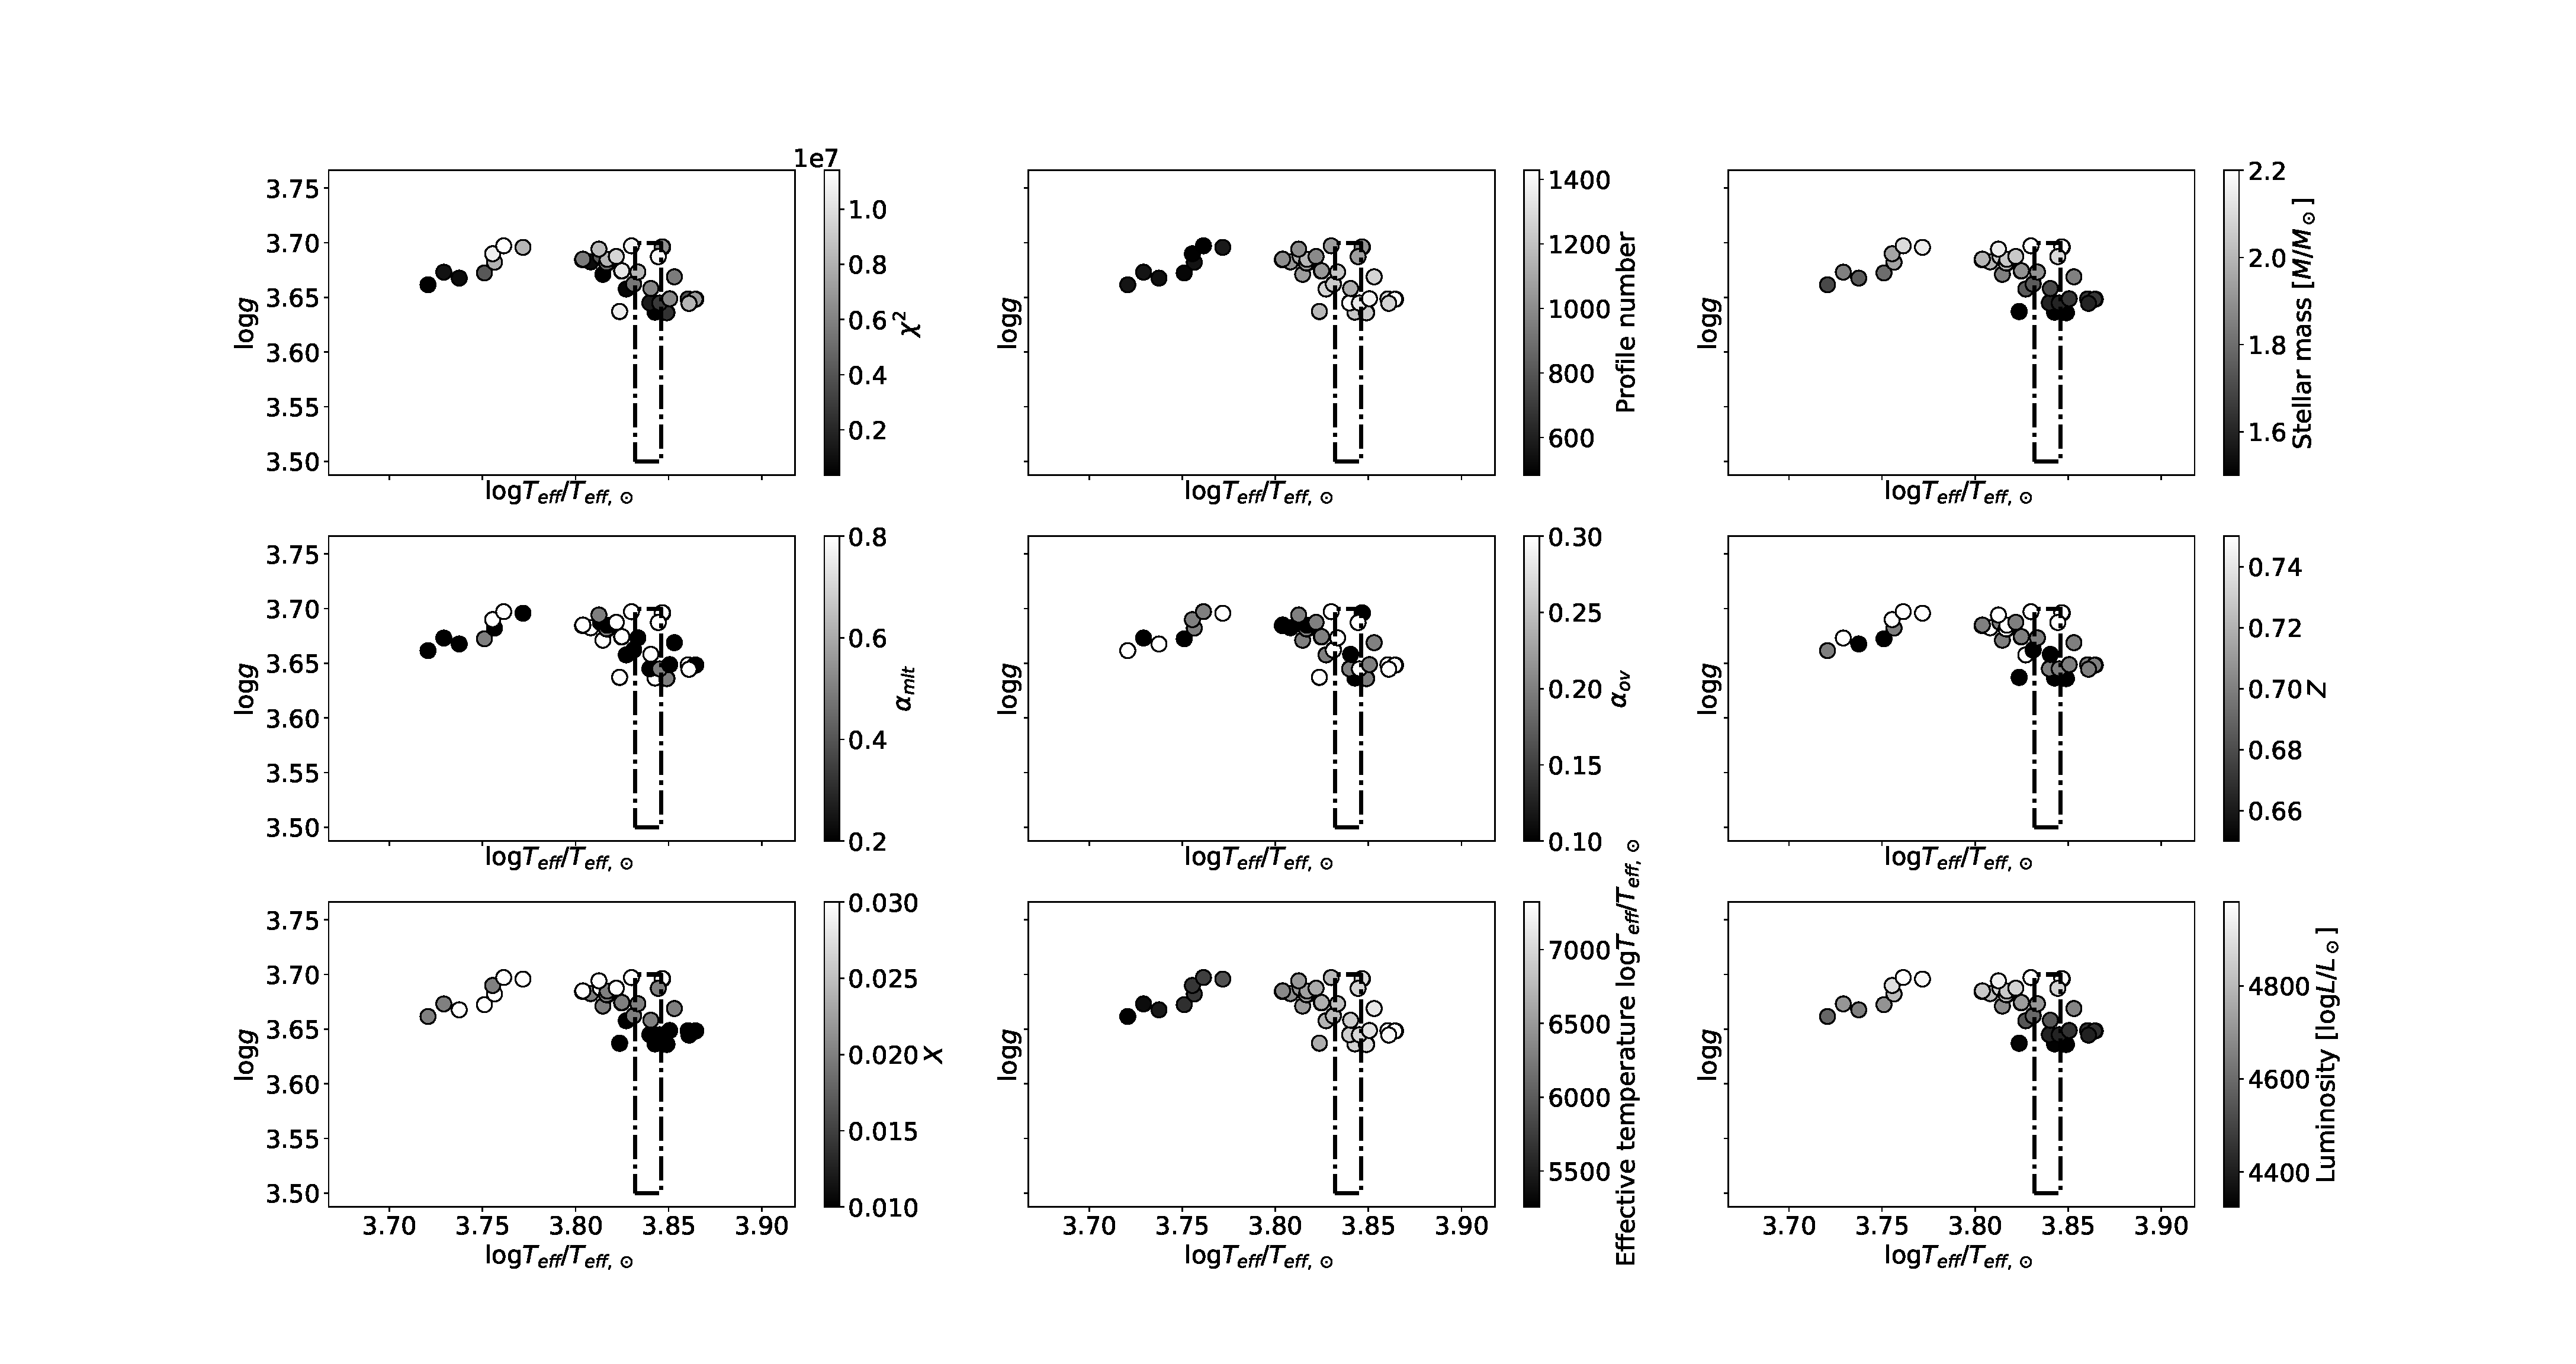
\includegraphics[width=1\textwidth]{scatter_all_v2.eps}
	\makebox[\textwidth][c]{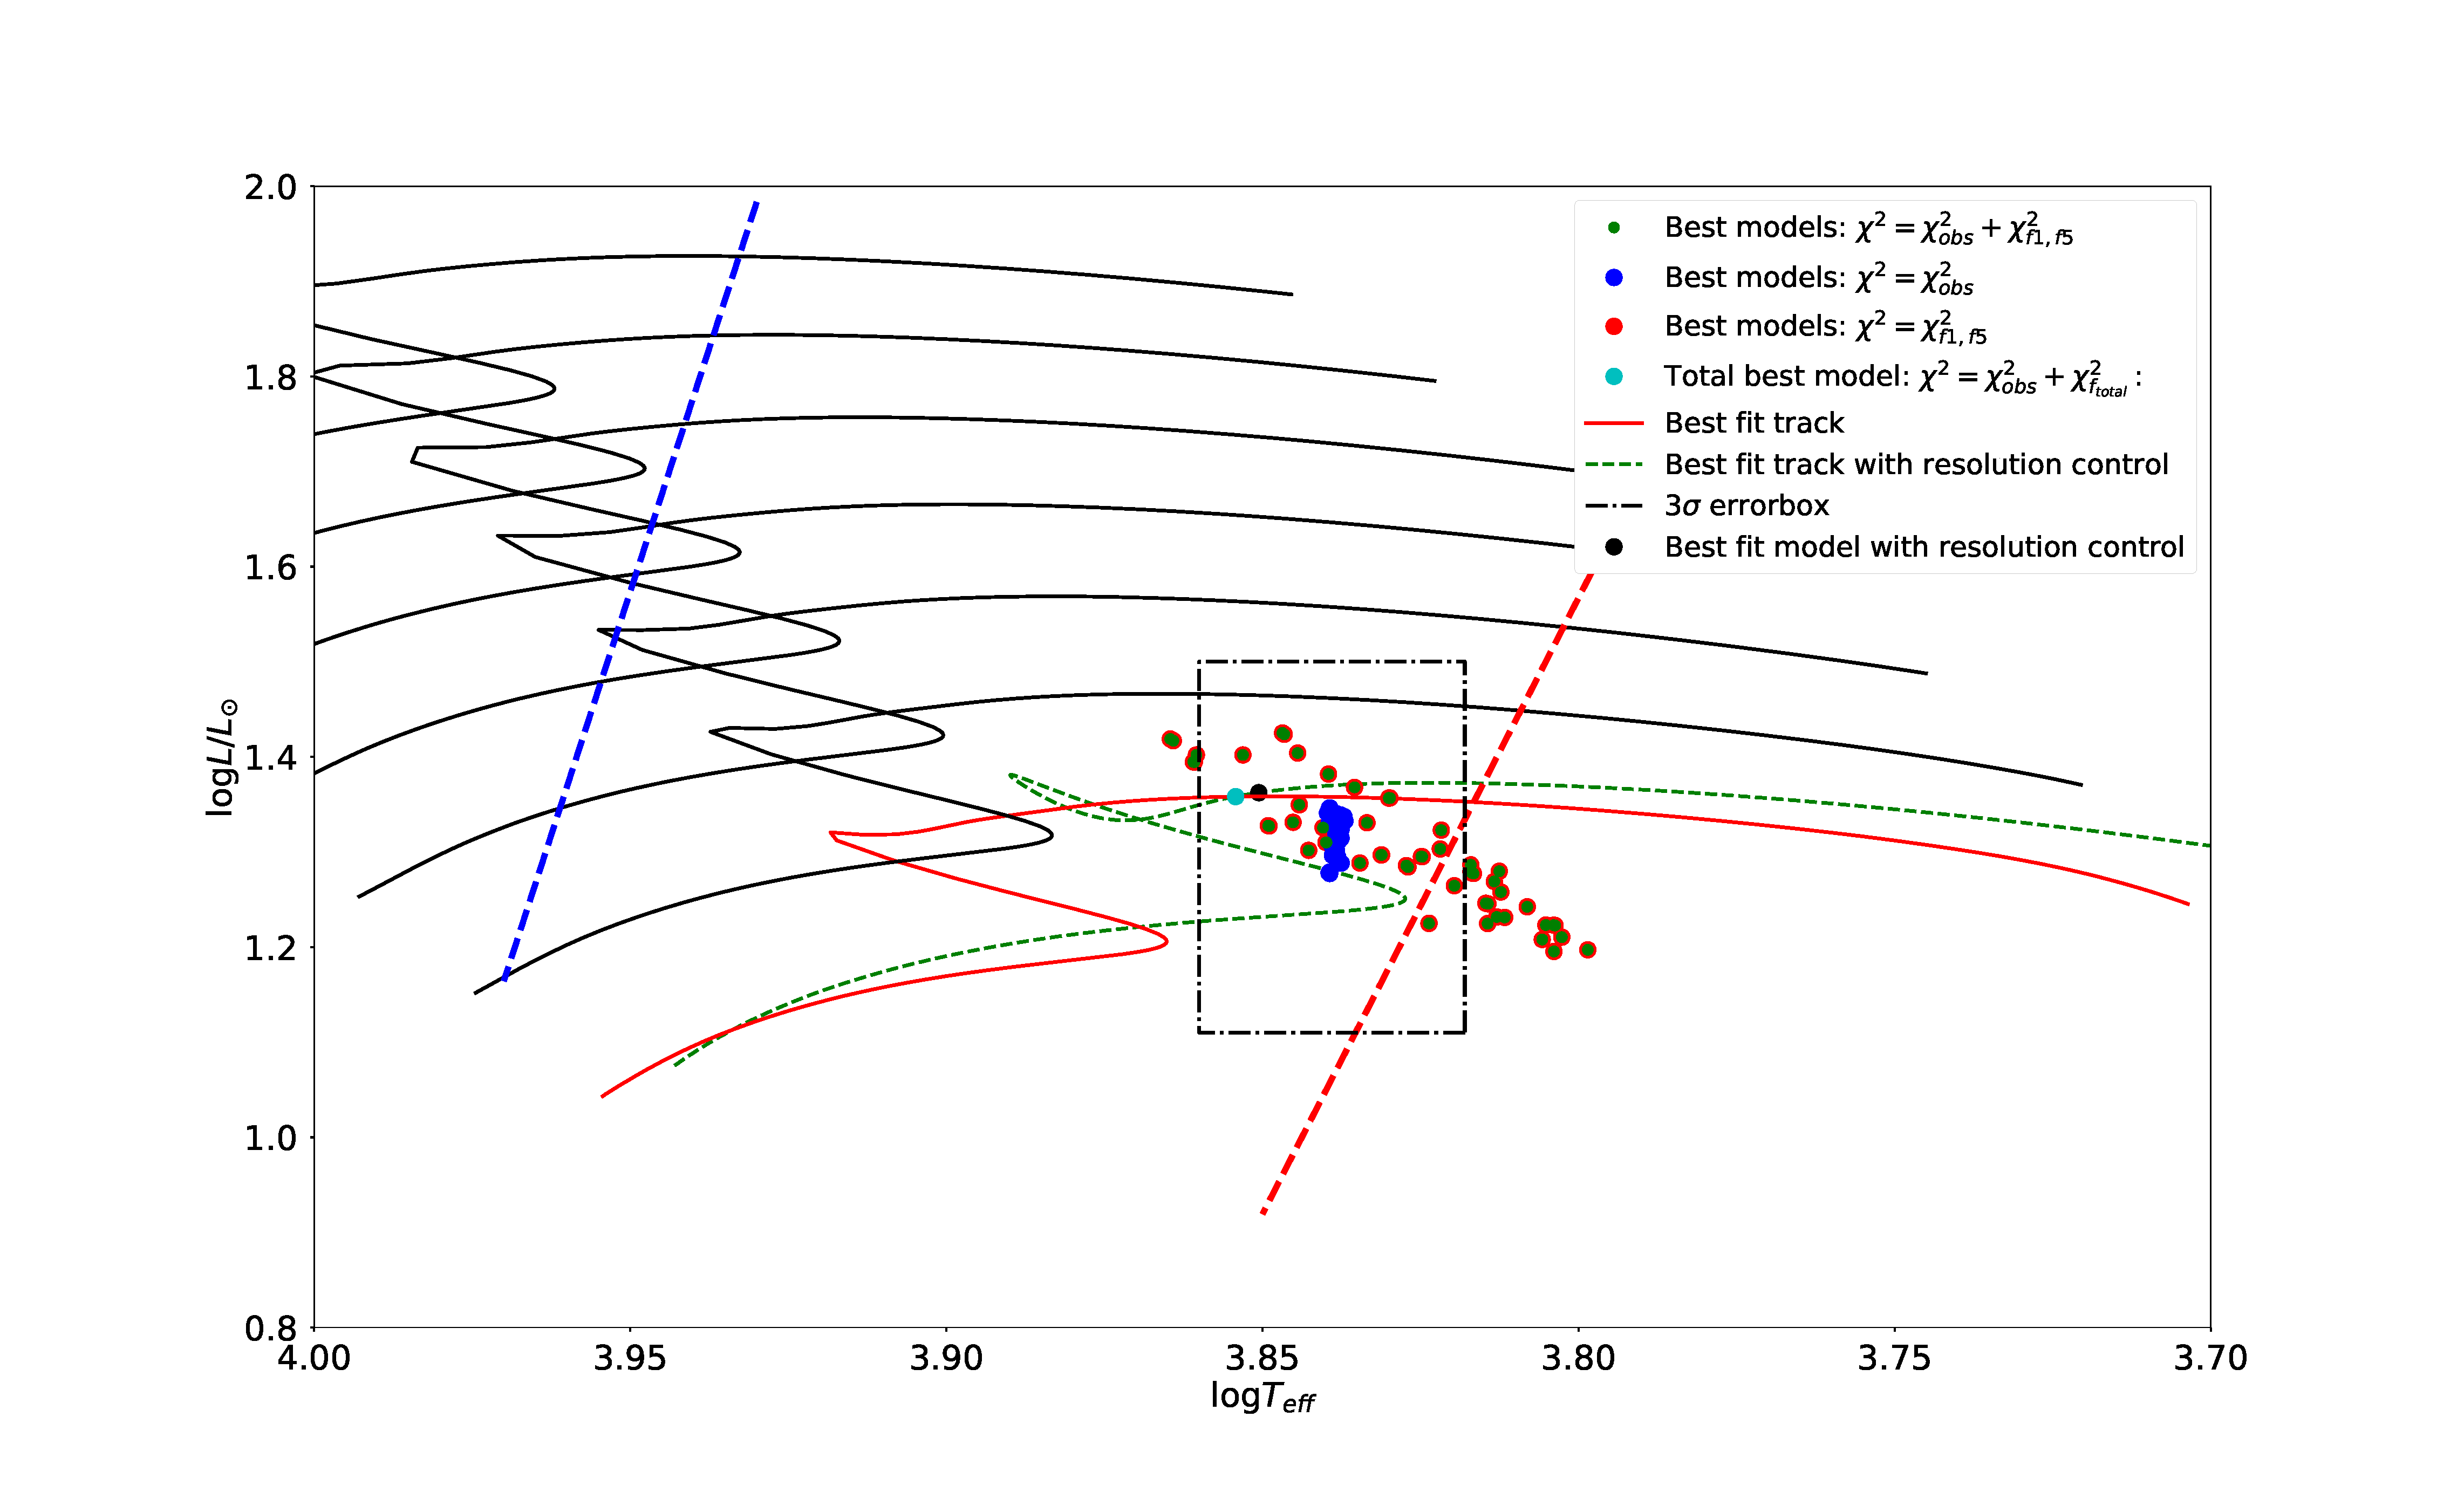
\includegraphics[width=1.3\textwidth]{final44tau.eps}}%
	\caption{HRD where the best model is estimated to be $M=1.55$\msun, $X=0.65$, $Z=0.01$, $\alpha_{mlt} = 0.5$, $\alpha_{ov} = 0.1$. The best total model is marked with a cyan blue dot, on the track marked with red. The green points shows the best 5\% models if the criteria is the total \chis. Blue dots are the 5\% best models if only observational parameters is included in the \chis, whereas the red dots is the 5\% if the \chis is only calculated from the frequency fits. The green tracks shows the best track with the black dot marking the best model if the frequency uncertainties have been artificially enhanced as in \eqref{sigma}. This track has the parameter combination of $M =2.05$ ,$X = 0.70$, $Z=0.03$, $\alpha_{mlt}=0.5$ and $\alpha_{ov}=0.3$.}
	\label{hrd44taulenz}
\end{figure}
The green points tend to overlap the red points, which again indicates that the frequencies are highly more weighted than the observational parameters. The frequencies thereby controls the final outcome, explaining why there is no difference in the main result by changing between the two runs for different observational parameter sets. 
%The best 5\% models from frequencies seems to be divided into two groups whereas the group near lower temperatures are models on the pre-ms. Since the pre-ms models were loaded from pre-calculated models as discussed in \chapref{compute}, causing different relaxation of the models, the pre-ms and particularly the frequencies on the pre-ms should not be trusted. Since the best model is between the other group it does not make a difference for the main result, but if further tests should be done with the 5\%, they should be excluded from the sample. 
The best model places 44 Tau on the post-MS, evolved further than result from \citet{lenz2010delta} whereas the best model with artificially pumped frequencies is earlier in its evolution. Both of these are within the three-sigma uncertainty of the observations (inside the errorbox). The frequency fit for the best model and best pumped model can be seen on \figref{freqfitbest}, \figref{freqfitpumped}, respectively. 
 
 \begin{figure}[htbp]
 	\centering
 	%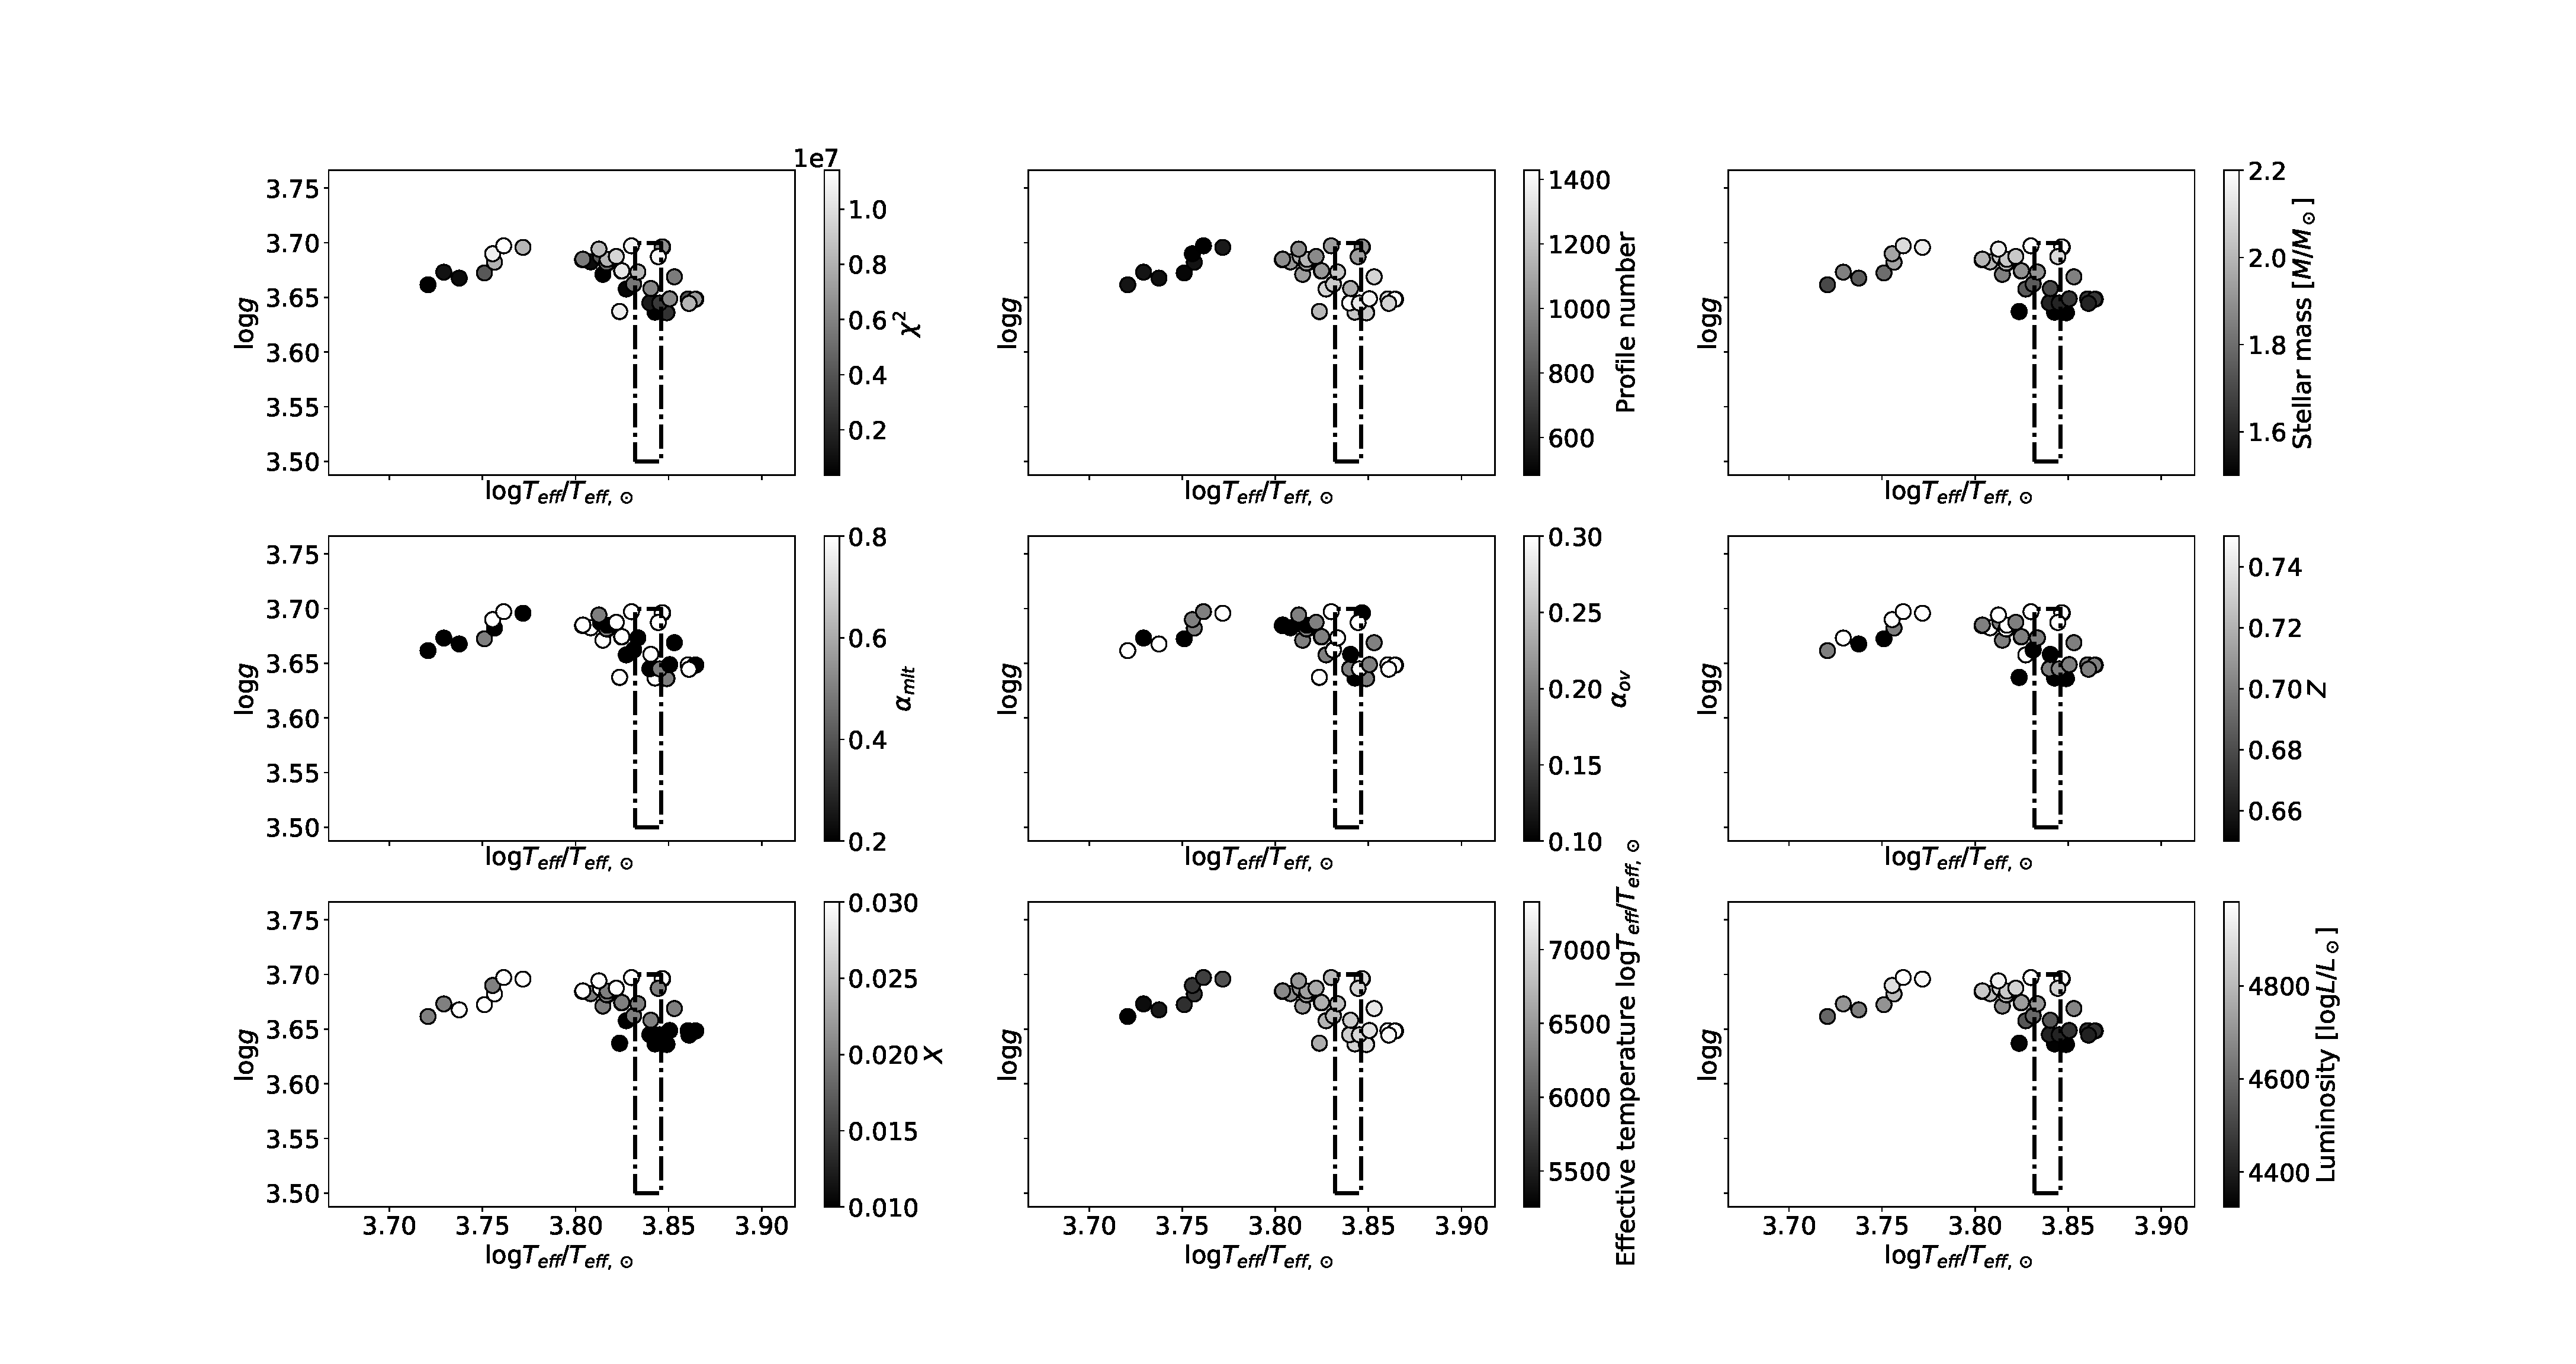
\includegraphics[width=1\textwidth]{scatter_all_v2.eps}
 	\makebox[\textwidth][c]{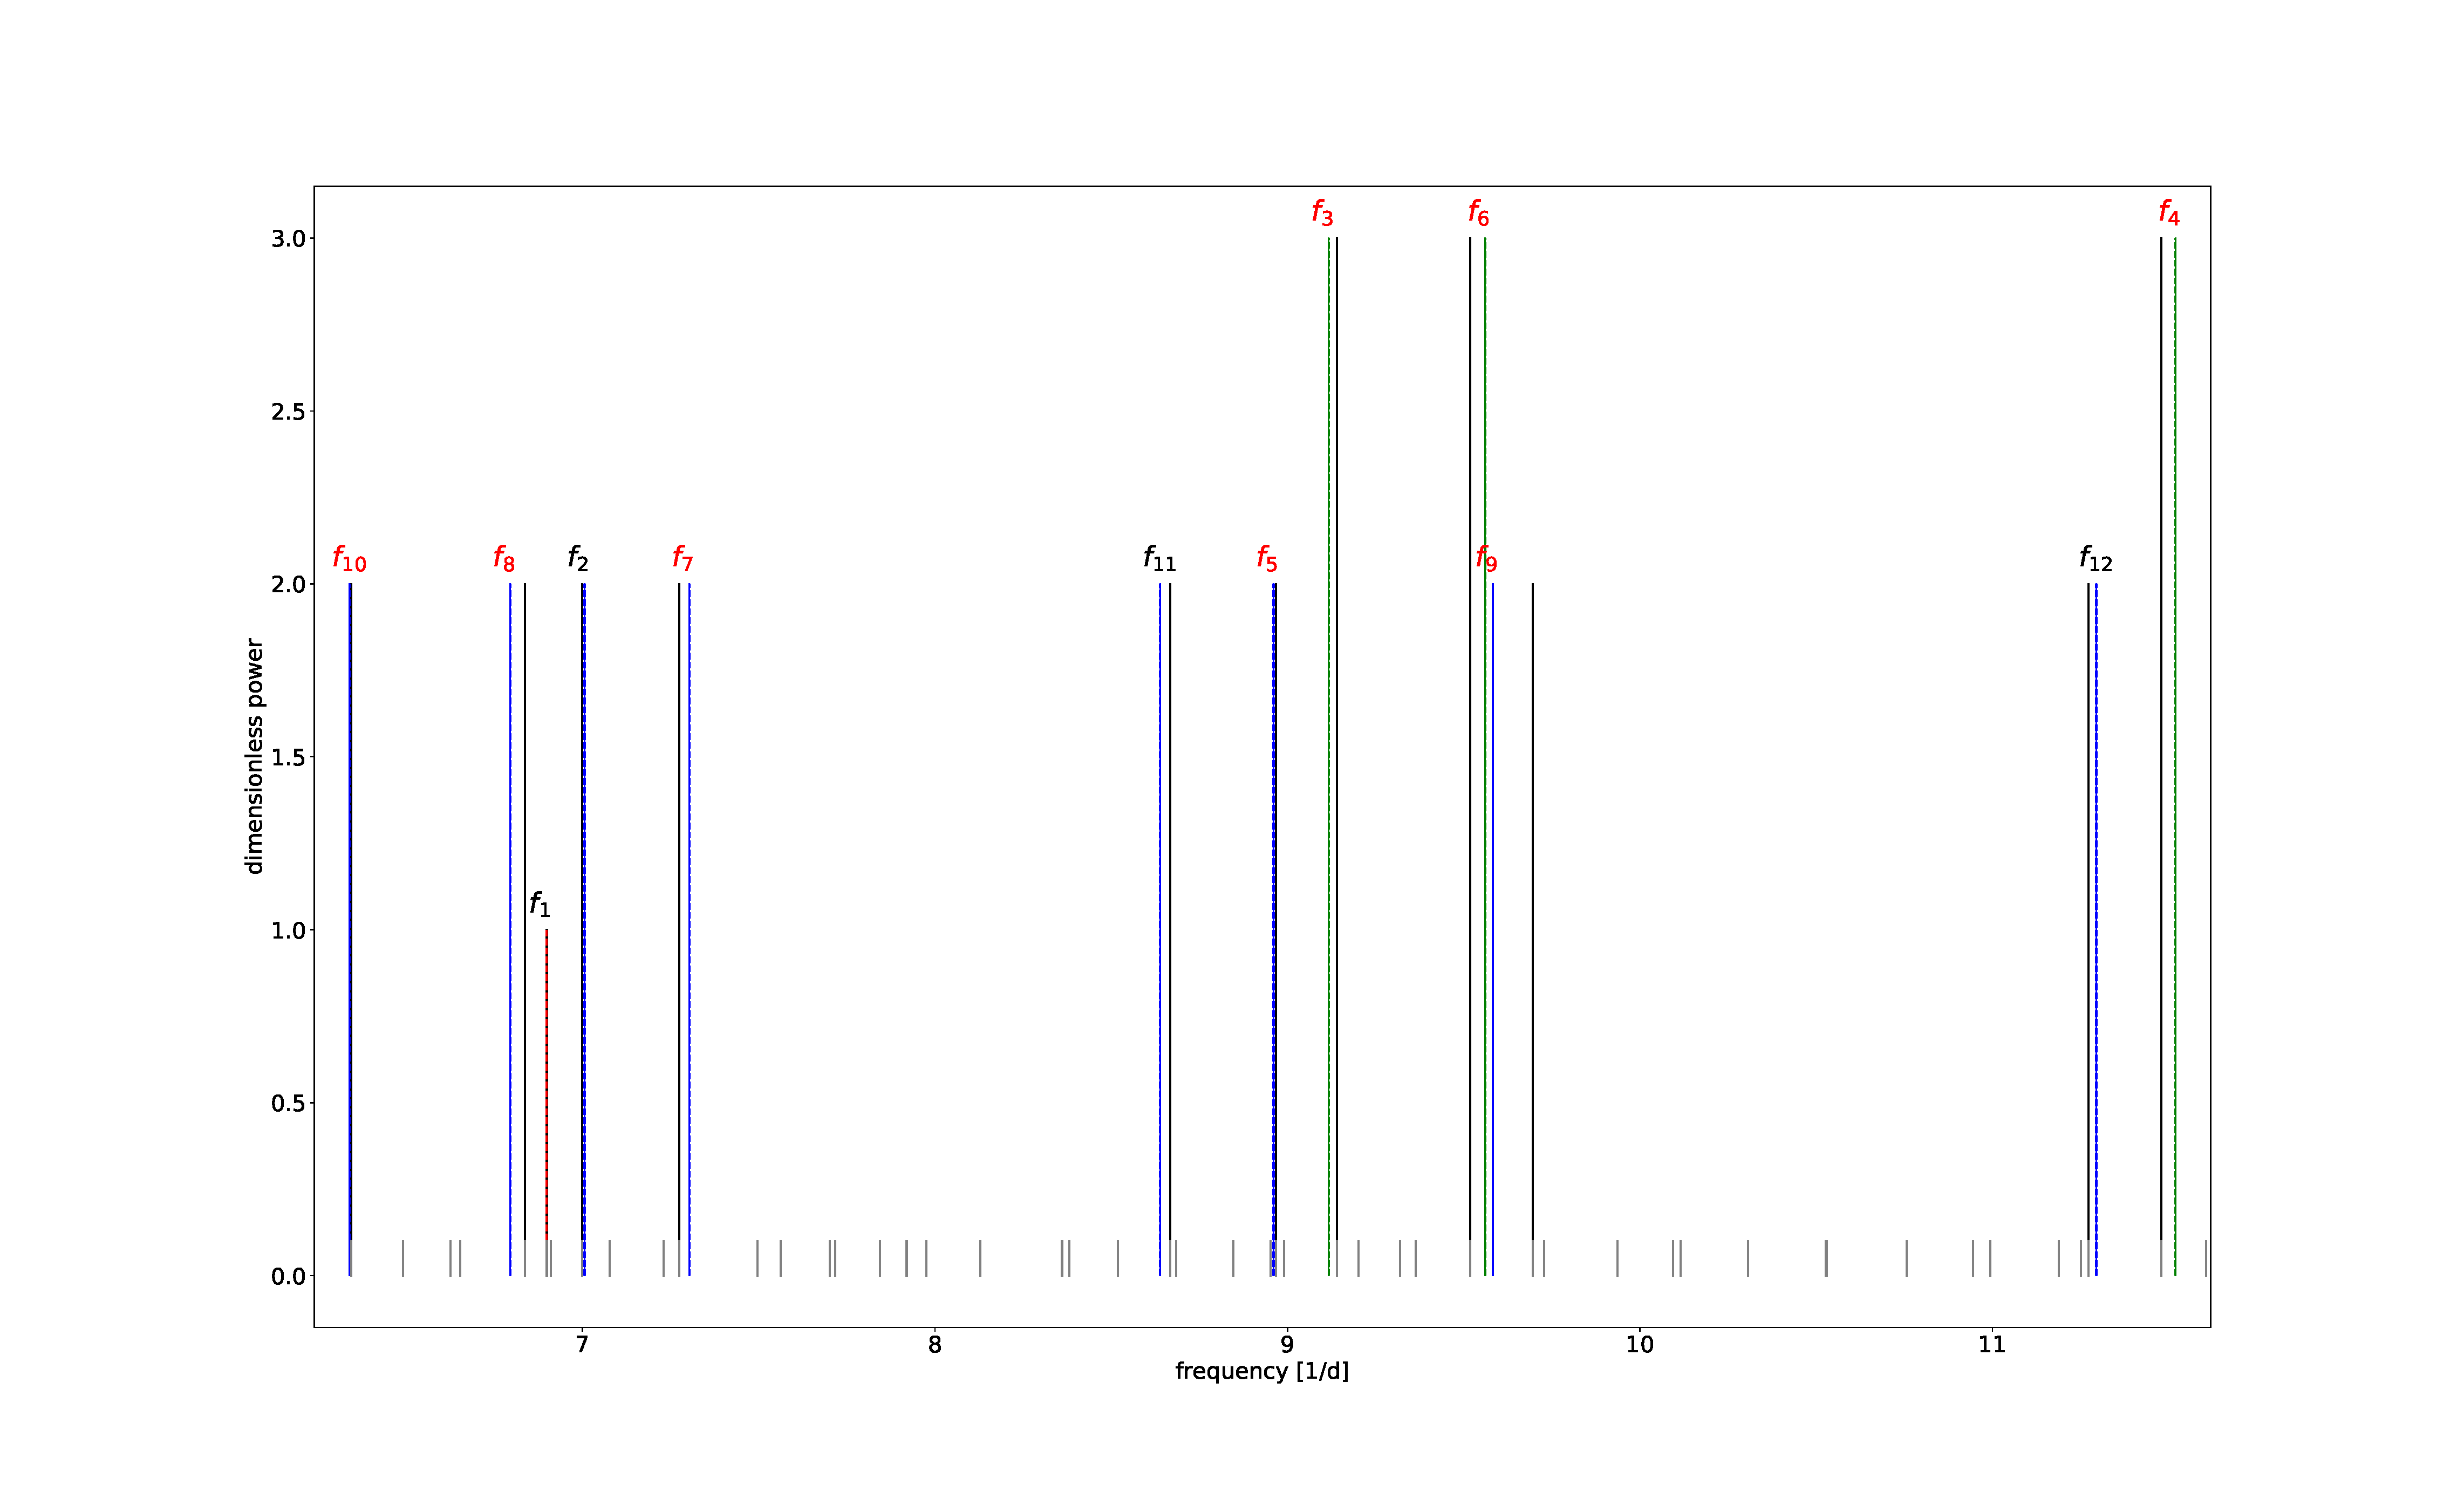
\includegraphics[width=1.2\textwidth]{freqsfit_bestmodel.eps}}%
 	\caption{Color-coded frequency plot of the best total model.  These are color-coded by the spherical degree as follows: $l=0$ are red, $l=1$ are blue and  $l=2$ are green, with dimensionless powers of 1,2 and 3. The black lines indicate the matched theoretical frequency, and the gray lines at the bottom represents all theoretically produced frequencies. The naming convention of the modes correspond to that of \citet{lenz2010delta}. Stippled lines are lines of uncertainty on the frequencies, although these are so small that they are not visible.}
 	\label{freqfitbest}
 \end{figure}
\begin{figure}[htbp]
	\centering
	%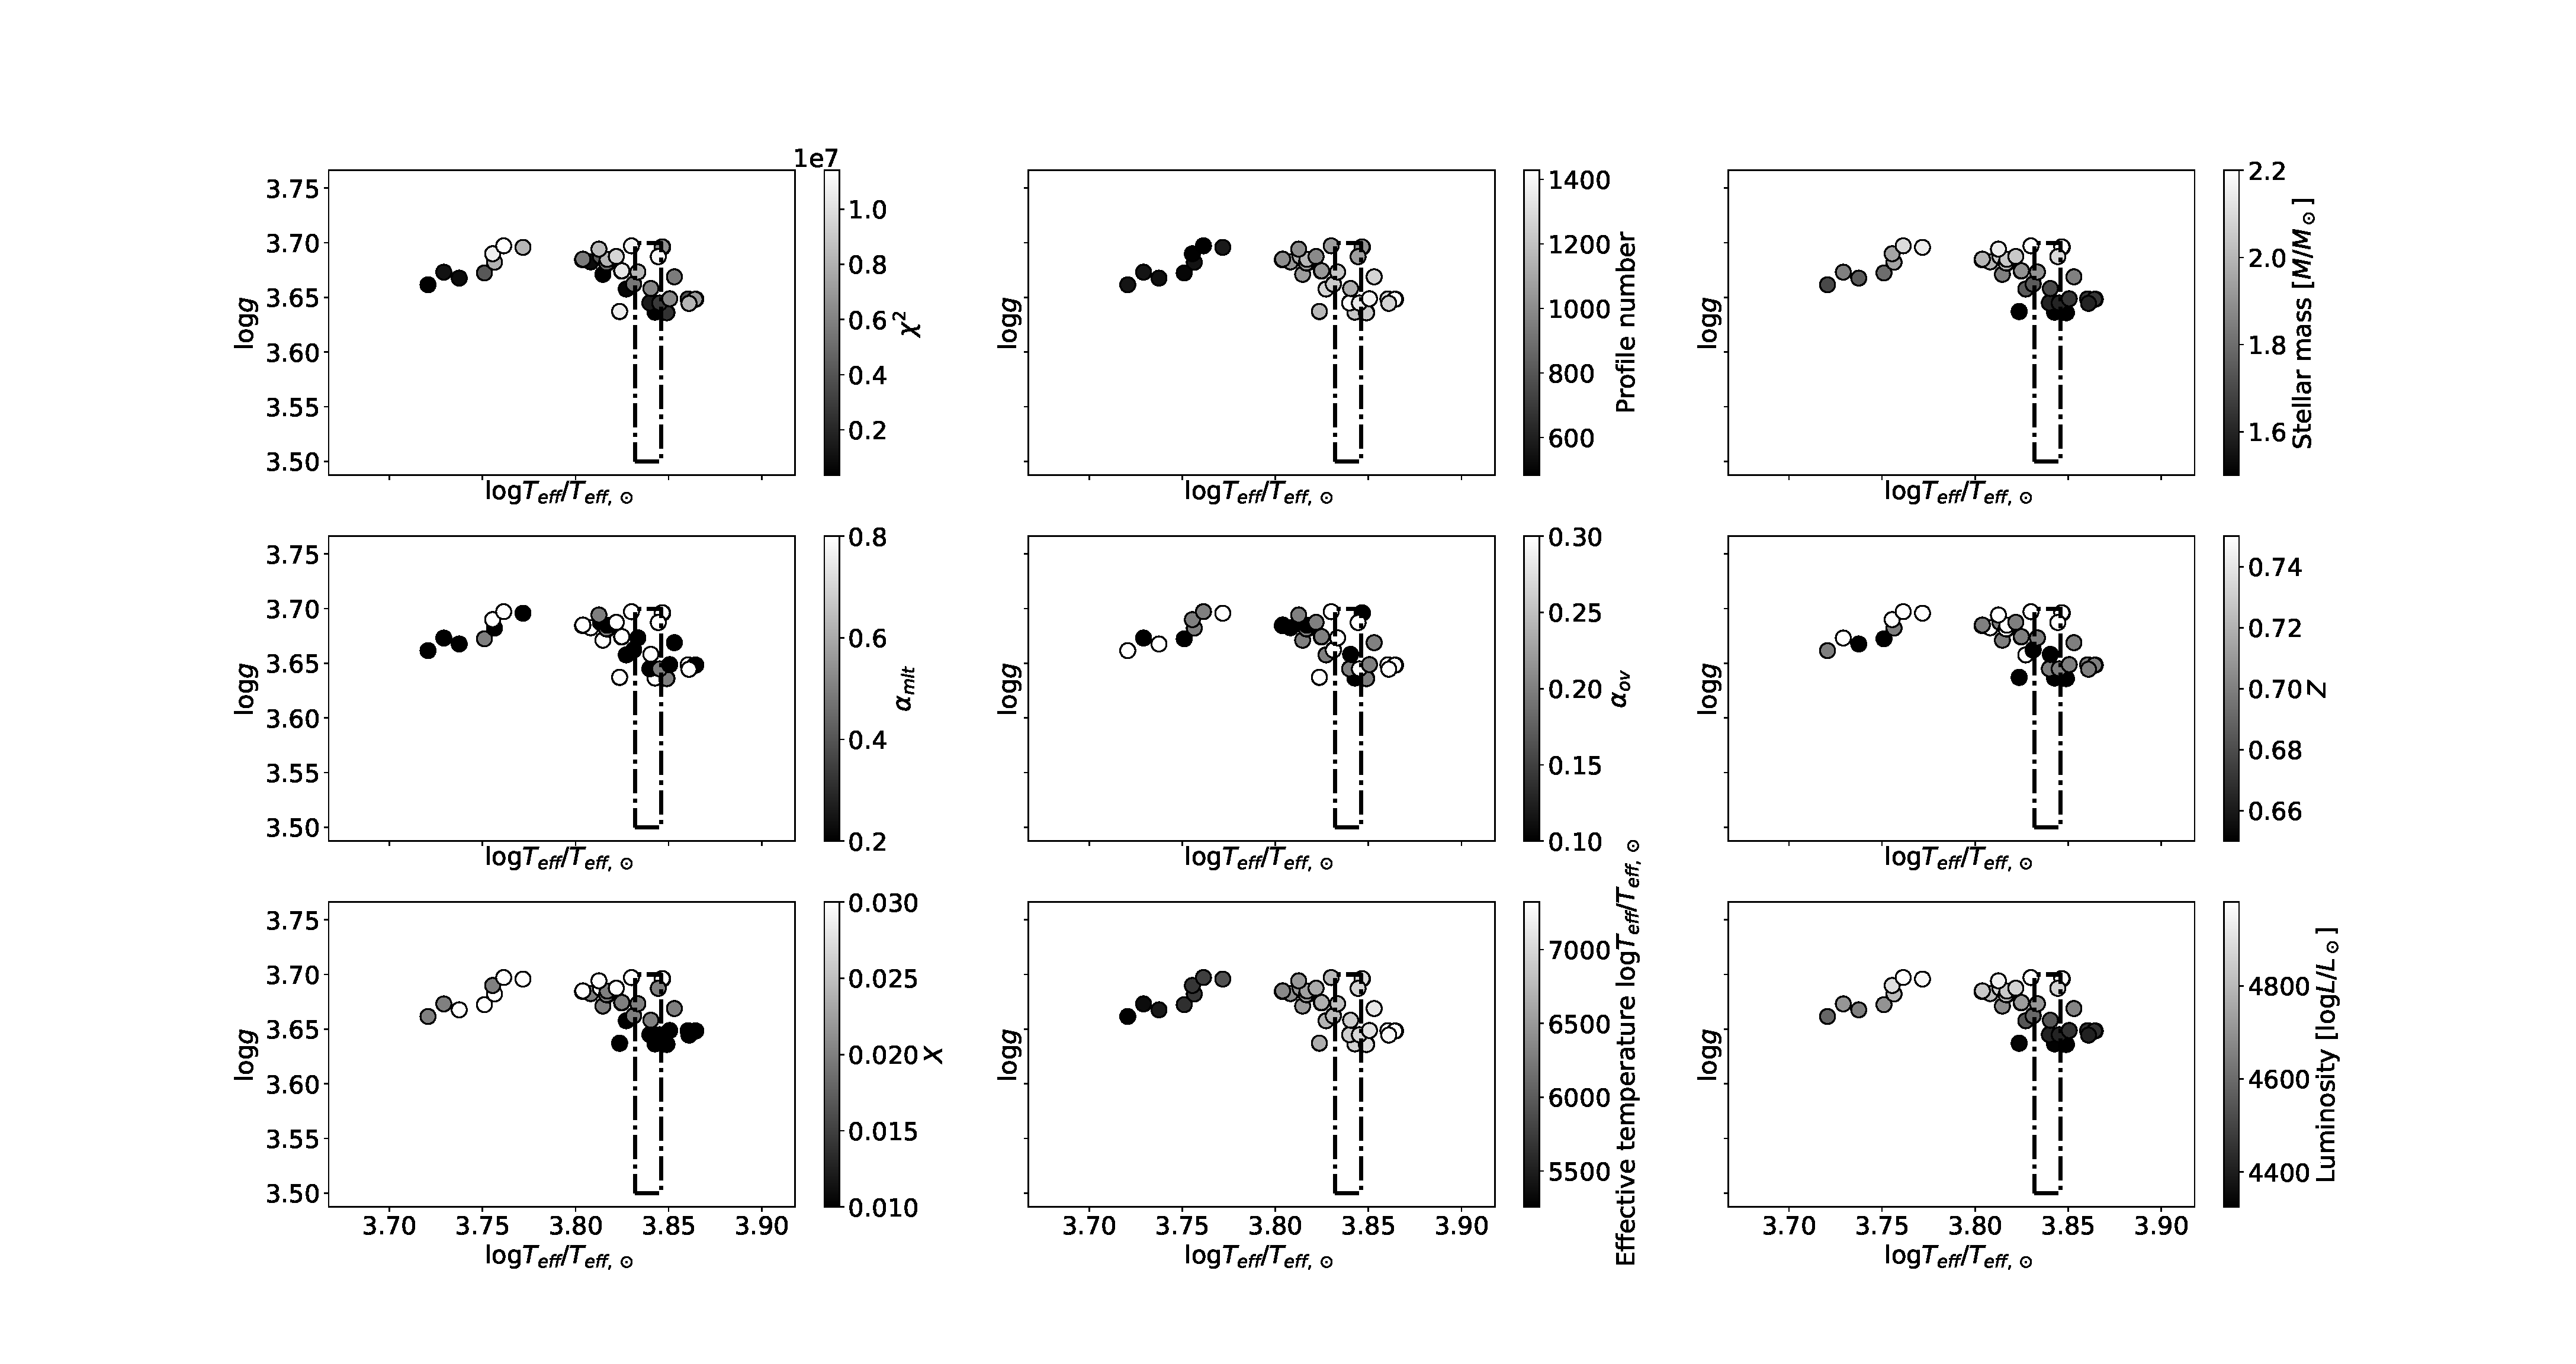
\includegraphics[width=1\textwidth]{scatter_all_v2.eps}
	\makebox[\textwidth][c]{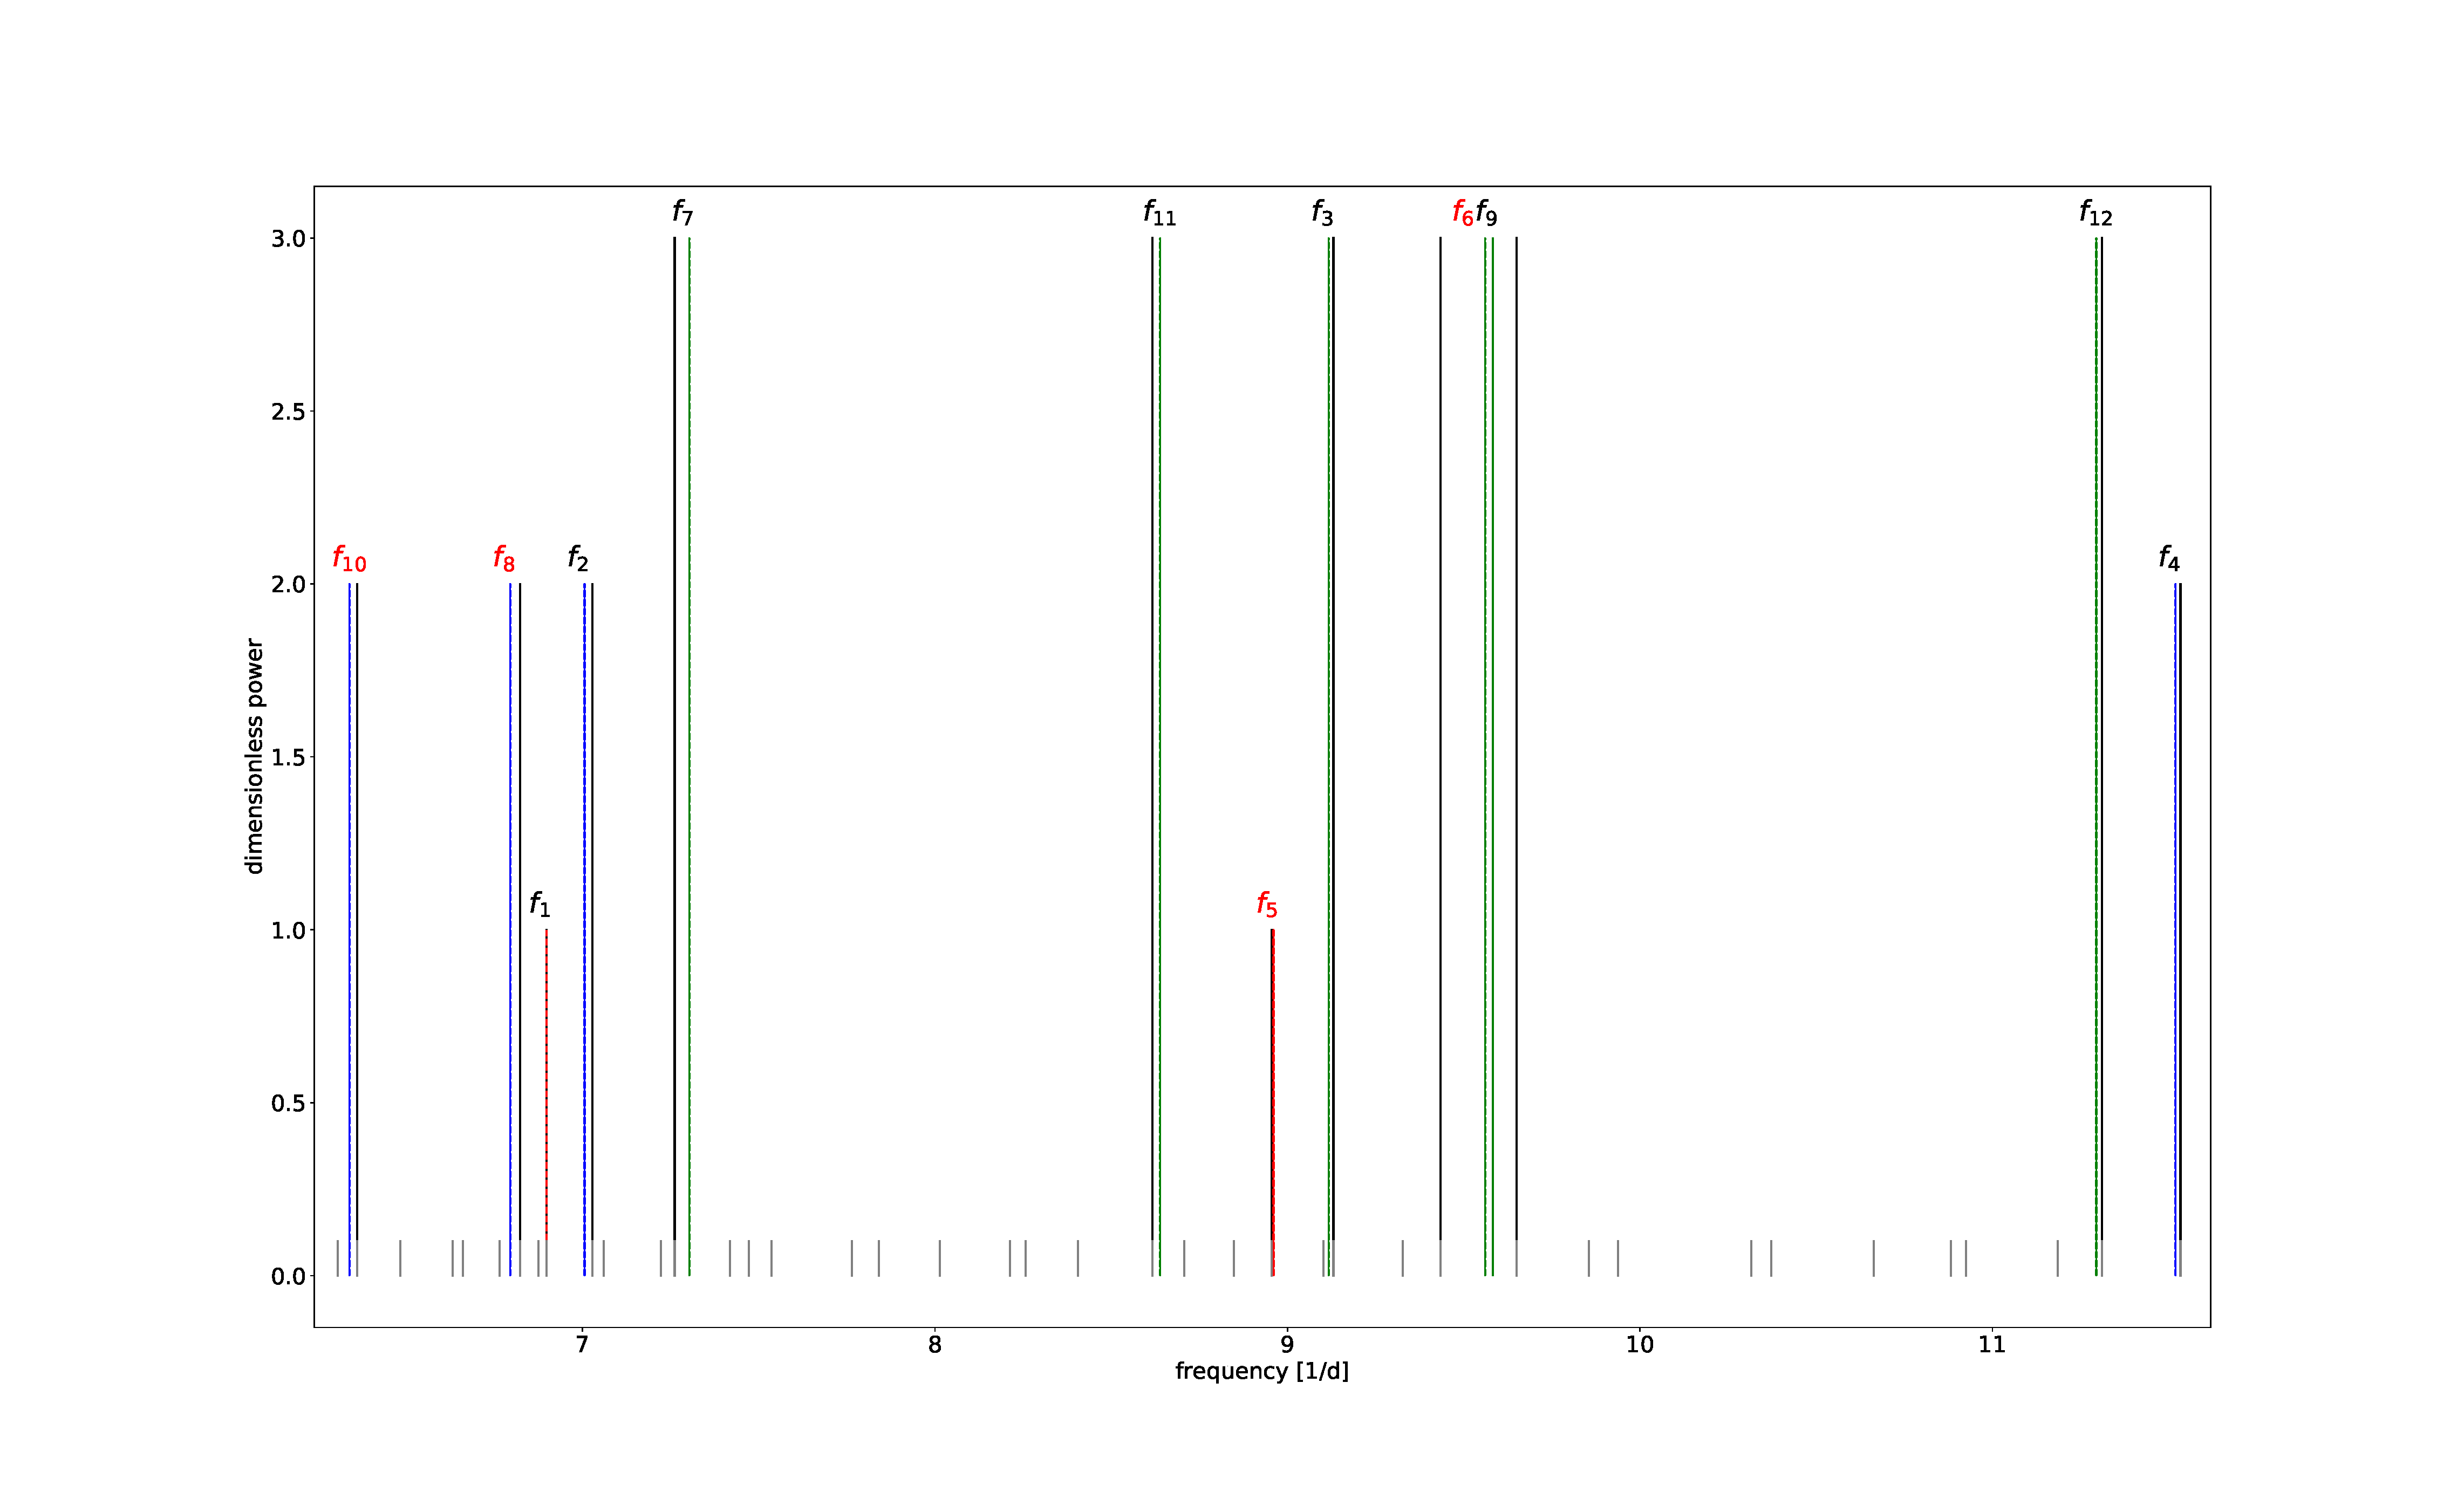
\includegraphics[width=1.2\textwidth]{freqsfit_bestpumped_2.eps}}%
	\caption{Frequency fit for best model with artificially enhanced uncertainties on the frequencies. Same color coding as \figref{freqfitbest}.}
	\label{freqfitpumped}
\end{figure}
 
 %Here, the observational frequencies are plotted with dimensionless power on the y-axis. They are color-coded by the spherical degree as follows: $l=0$ are red, $l=1$ are blue and  $l=2$ are green, with dimensionless powers of 1,2 and 3. The black lines indicate the matched theoretical frequency, and the gray lines at the bottom represents all theoretically produced frequencies.
  The naming convention of the frequencies are defined as in \tabref{freqs}. Stippled lines are lines of uncertainty on the frequencies, although these are so small that they are not visible. Since the uncertainty is so small, technically none of the theoretical frequencies are matched within the uncertainties. However, they are all matched within a range of $0.2 d^{-1}$. The text marked with red are indicates where the estimated modes from mode identification is different from the theoretically calculated spherical degrees. To indicate that some models might be better estimates for the star, a frequency fit of the track $M=1.65$, $X=0.70$, $Z=0.01$, $\alpha_{mlt} = 0.5$, $\alpha_{ov}=0.3$ is shown of \figref{freqfit}\footnote{This run includes pre-MS models as well. These do not influence the minimum \chis of this run}. Here, only two modes could differ in spherical degree from the mode identification. The corresponding HRD is shown on \figref{hrd44old}. Here, the evolutionary stage is pushed back to the Henyey hook, closer to the results of \citet{lenz2010delta}\footnote{This run was made without the cutoff at profile > 900, meaning that pre-MS models are included. They are located at the bottom right corner}. Therefore, for future work it is necessary to implement a routine weighing the different frequencies depending on the mode identification as well. 
 
  There can be other reasons for the contradictions in spherical degree : 1) The pulsation code does not calculate the theoretically produced frequencies correctly. At this point it is already a well-known issue that the theory behind these type of oscillations does not comply well with observations. \citet{lenz2010delta} was indeed successful with modeling 44 Tau, but this example is the first one of its kind where all identified modes where reproduced theoretically. More often, pulsation codes does not match observations. 2) Due to the high uncertainty in mode identification, some of the modes have been misidentified. This is the more likely scenario since 1) would probably cause issues for more than two modes, and would not have been able to fit the rest either. There is also strong evidence that some modes could be identified wrongly due to the model dependency of the mode identification. It can be seen on \figref{lenzdiss} that the choice of mixing length affects the mode identification significantly. The theoretically predicted regions for $l=0,1,2$ are marked with red, green and blue respectively. Observations are plotted with black boxes. For small values of $\alpha_{mlt}$ the regions tend to move closer, making it difficult to distinguish between spherical degree. These models are based on frozen convection where the mixing length describes the local convection. However, time-dependent convection is needed in order to describe the full picture of convection, and the difference in mode identification is significant \citep{dupret2005time},(Victoria Antoci 2019, private communication).
\begin{figure}[htbp]
	\centering
	%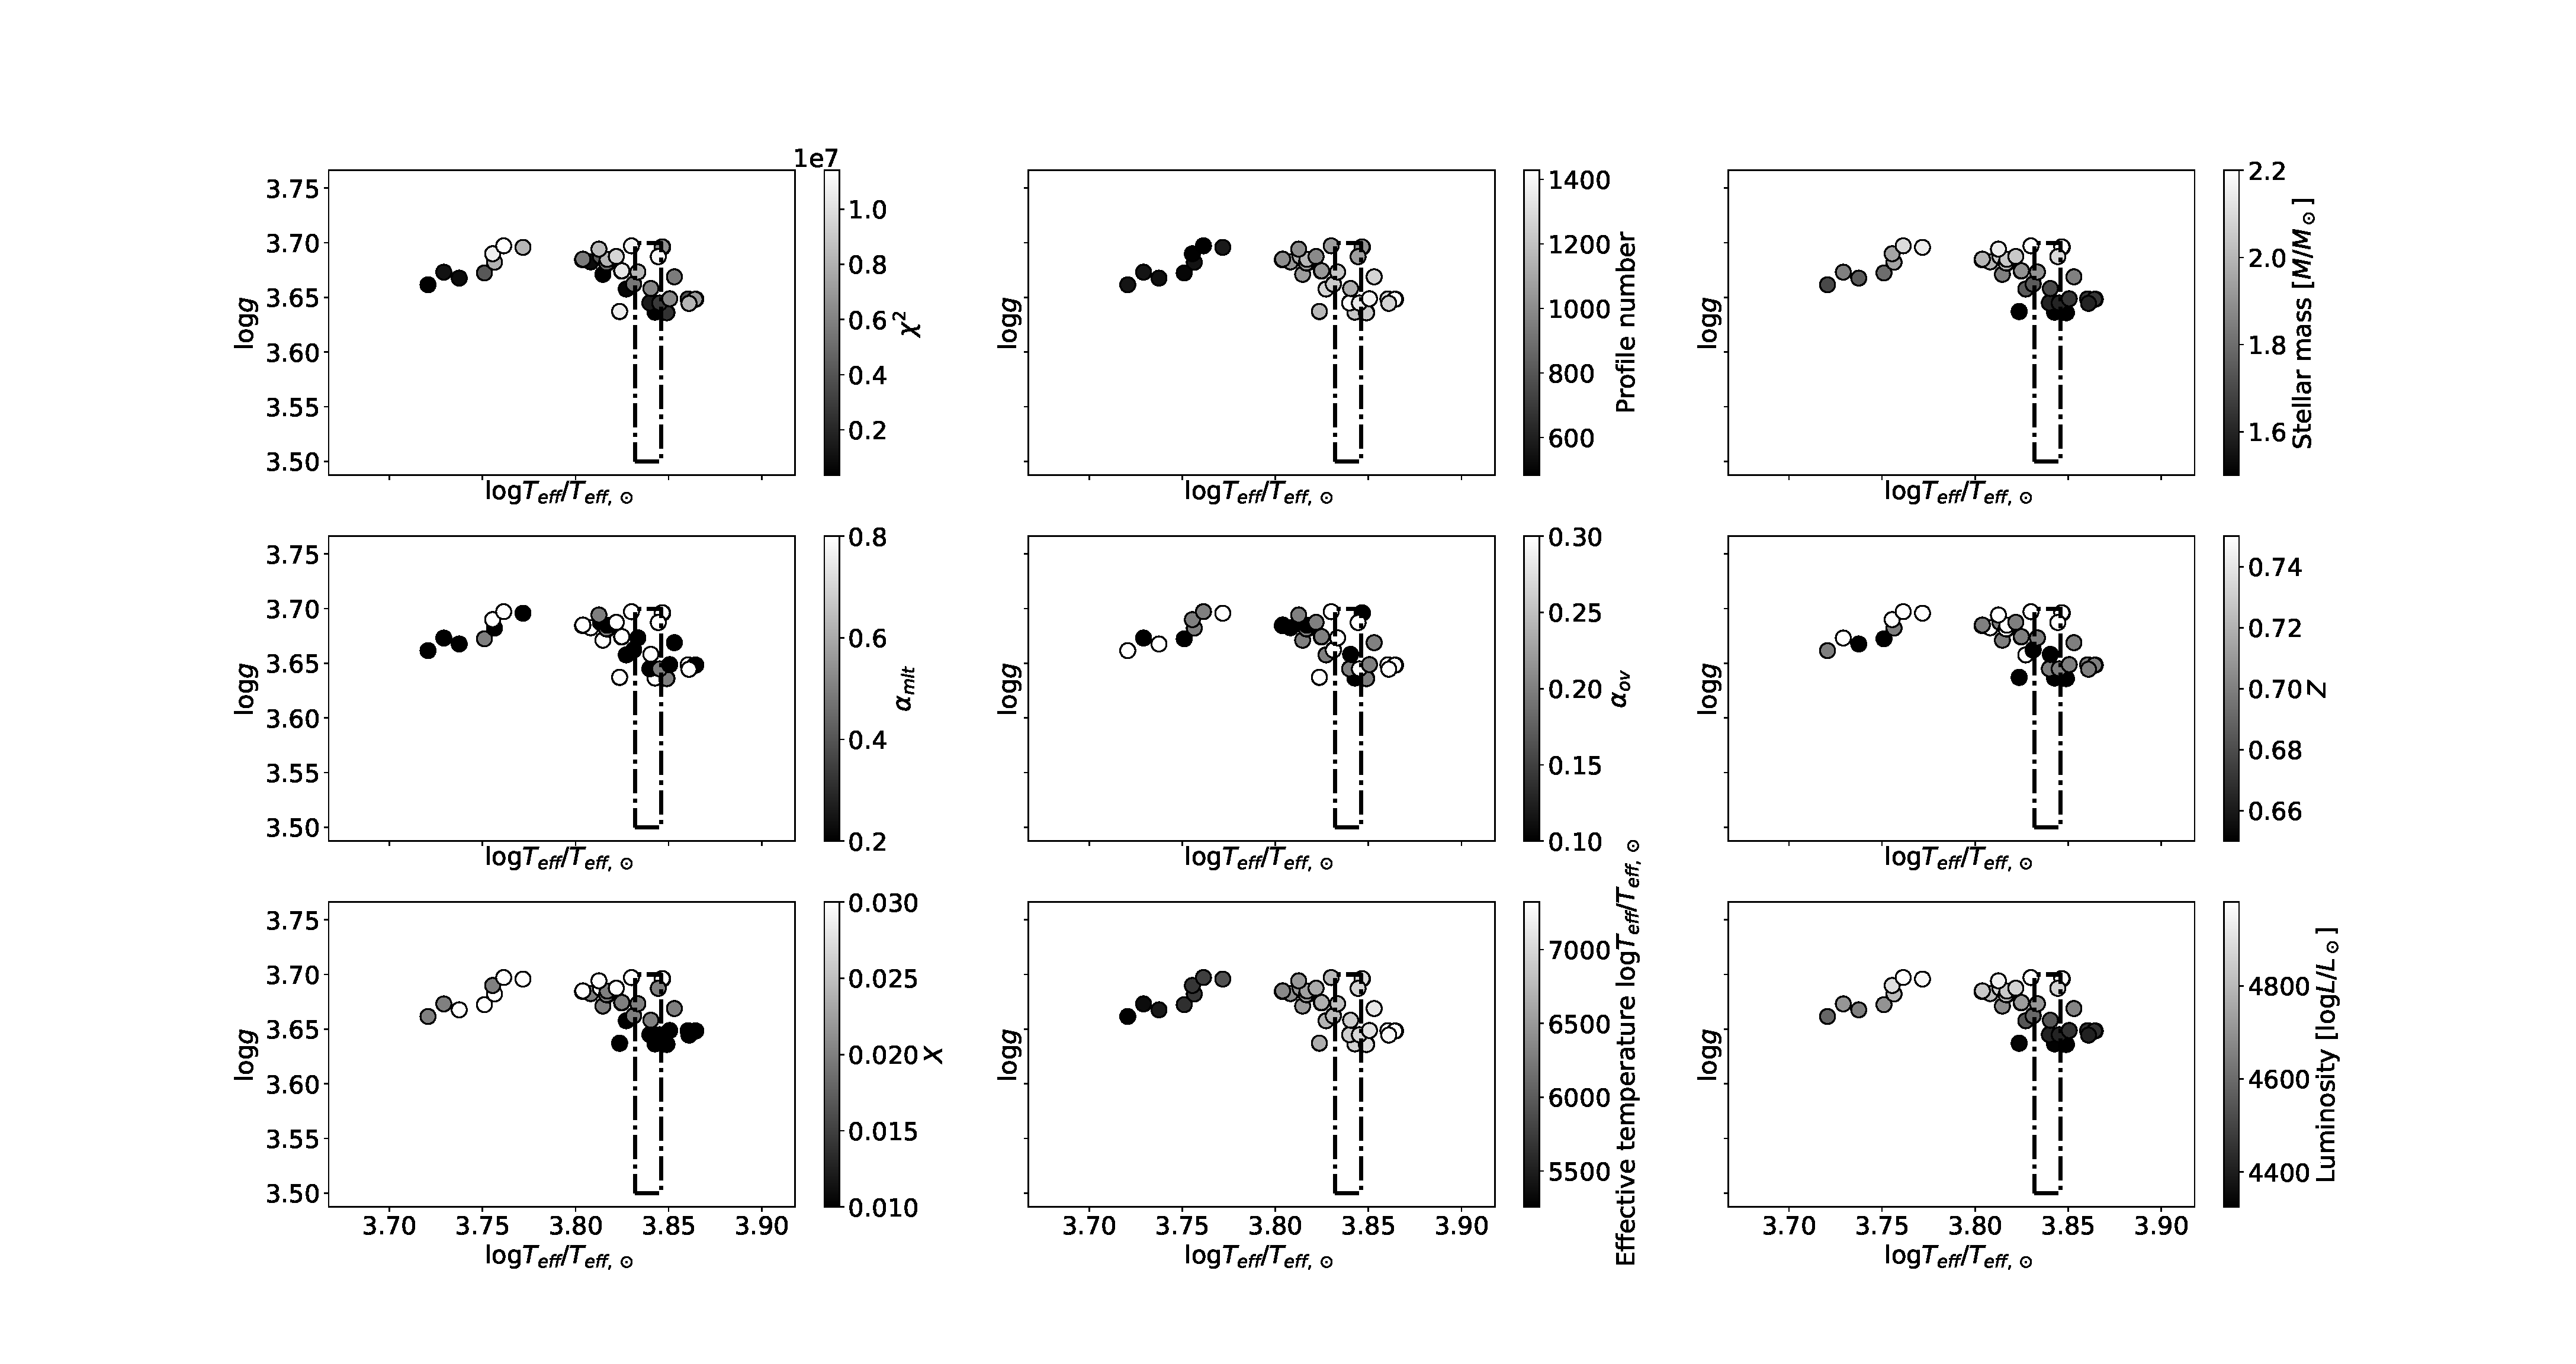
\includegraphics[width=1\textwidth]{scatter_all_v2.eps}
	\makebox[\textwidth][c]{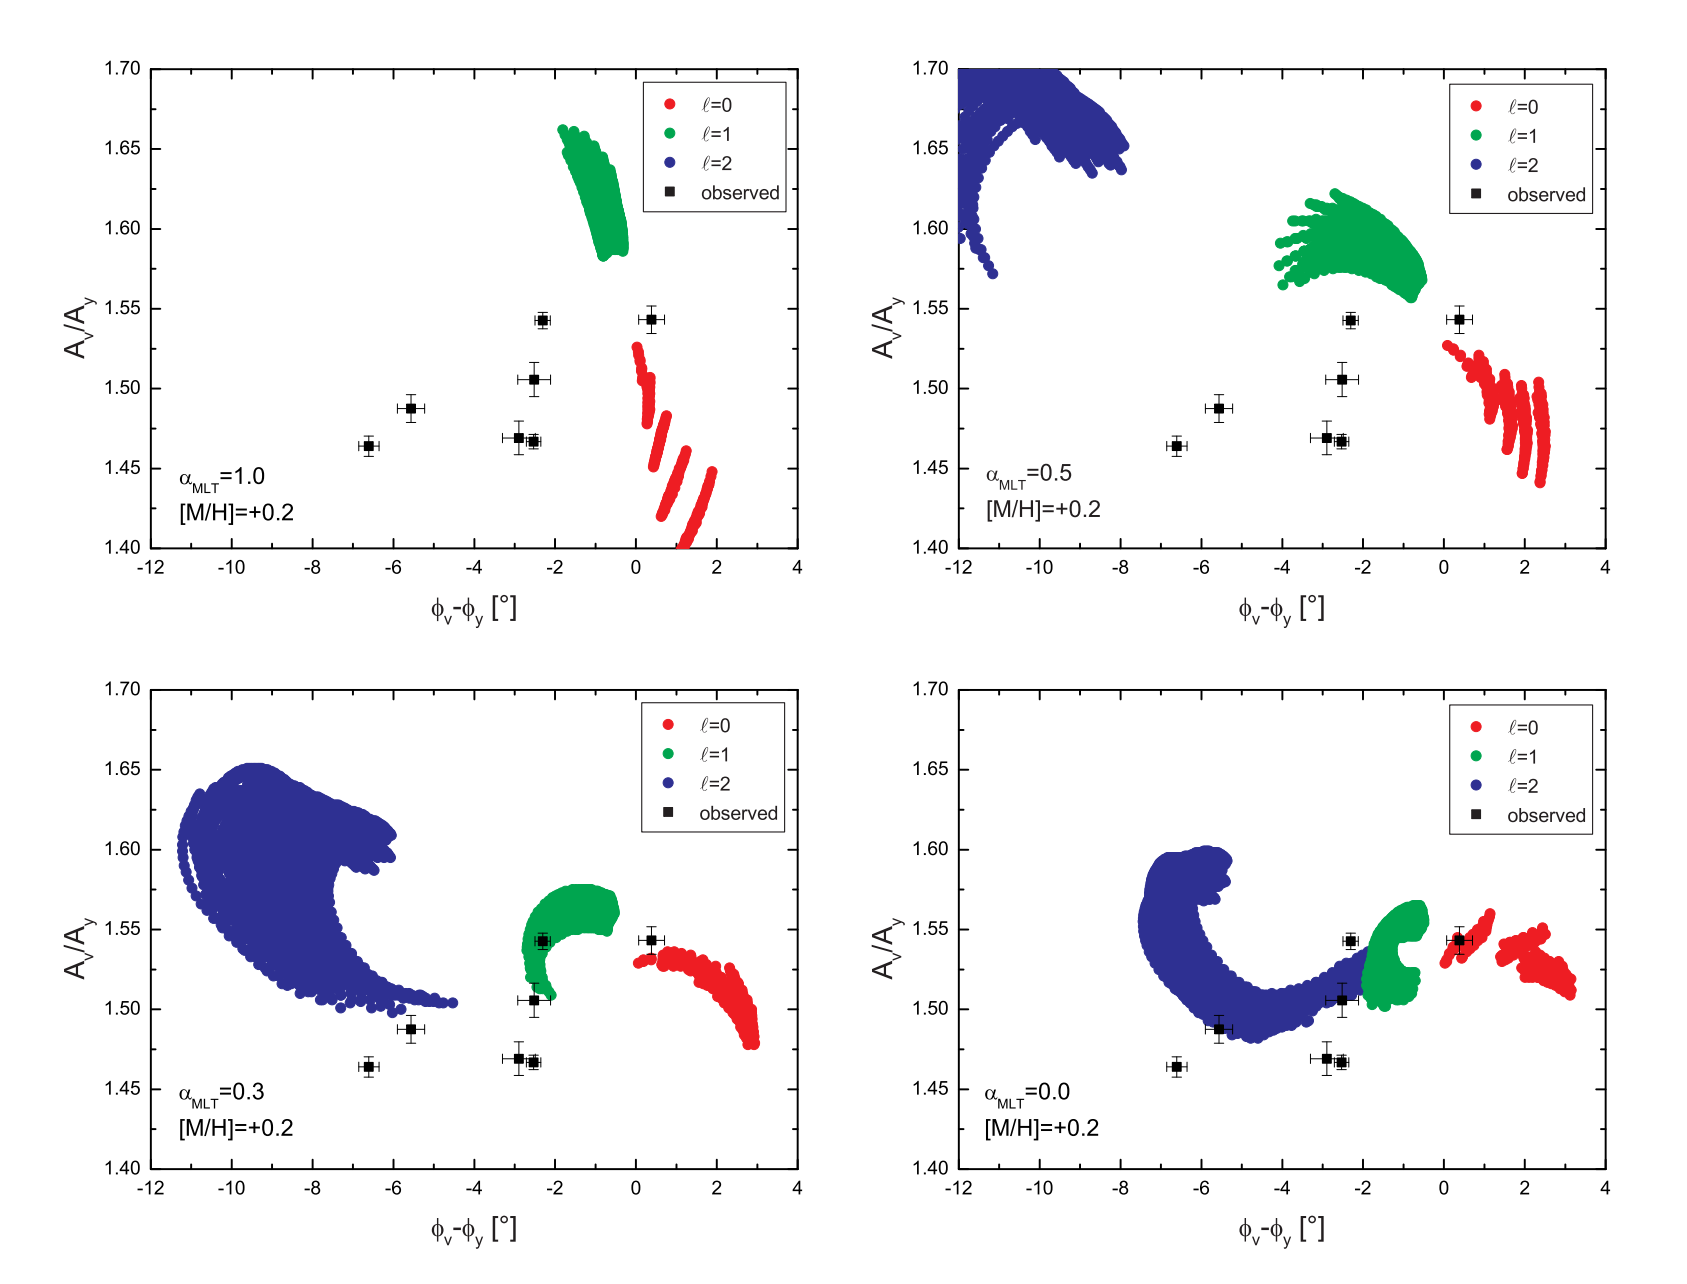
\includegraphics[width=1\textwidth]{lenzdiss.png}}%
	\caption{Predicted theoretical model position for four different values of the mixing length parameter $\alpha_{mlt}$.  Figure from \citet{lenz2009diss}  }
	\label{lenzdiss}
\end{figure}
\begin{figure}[htbp]
	\centering
	%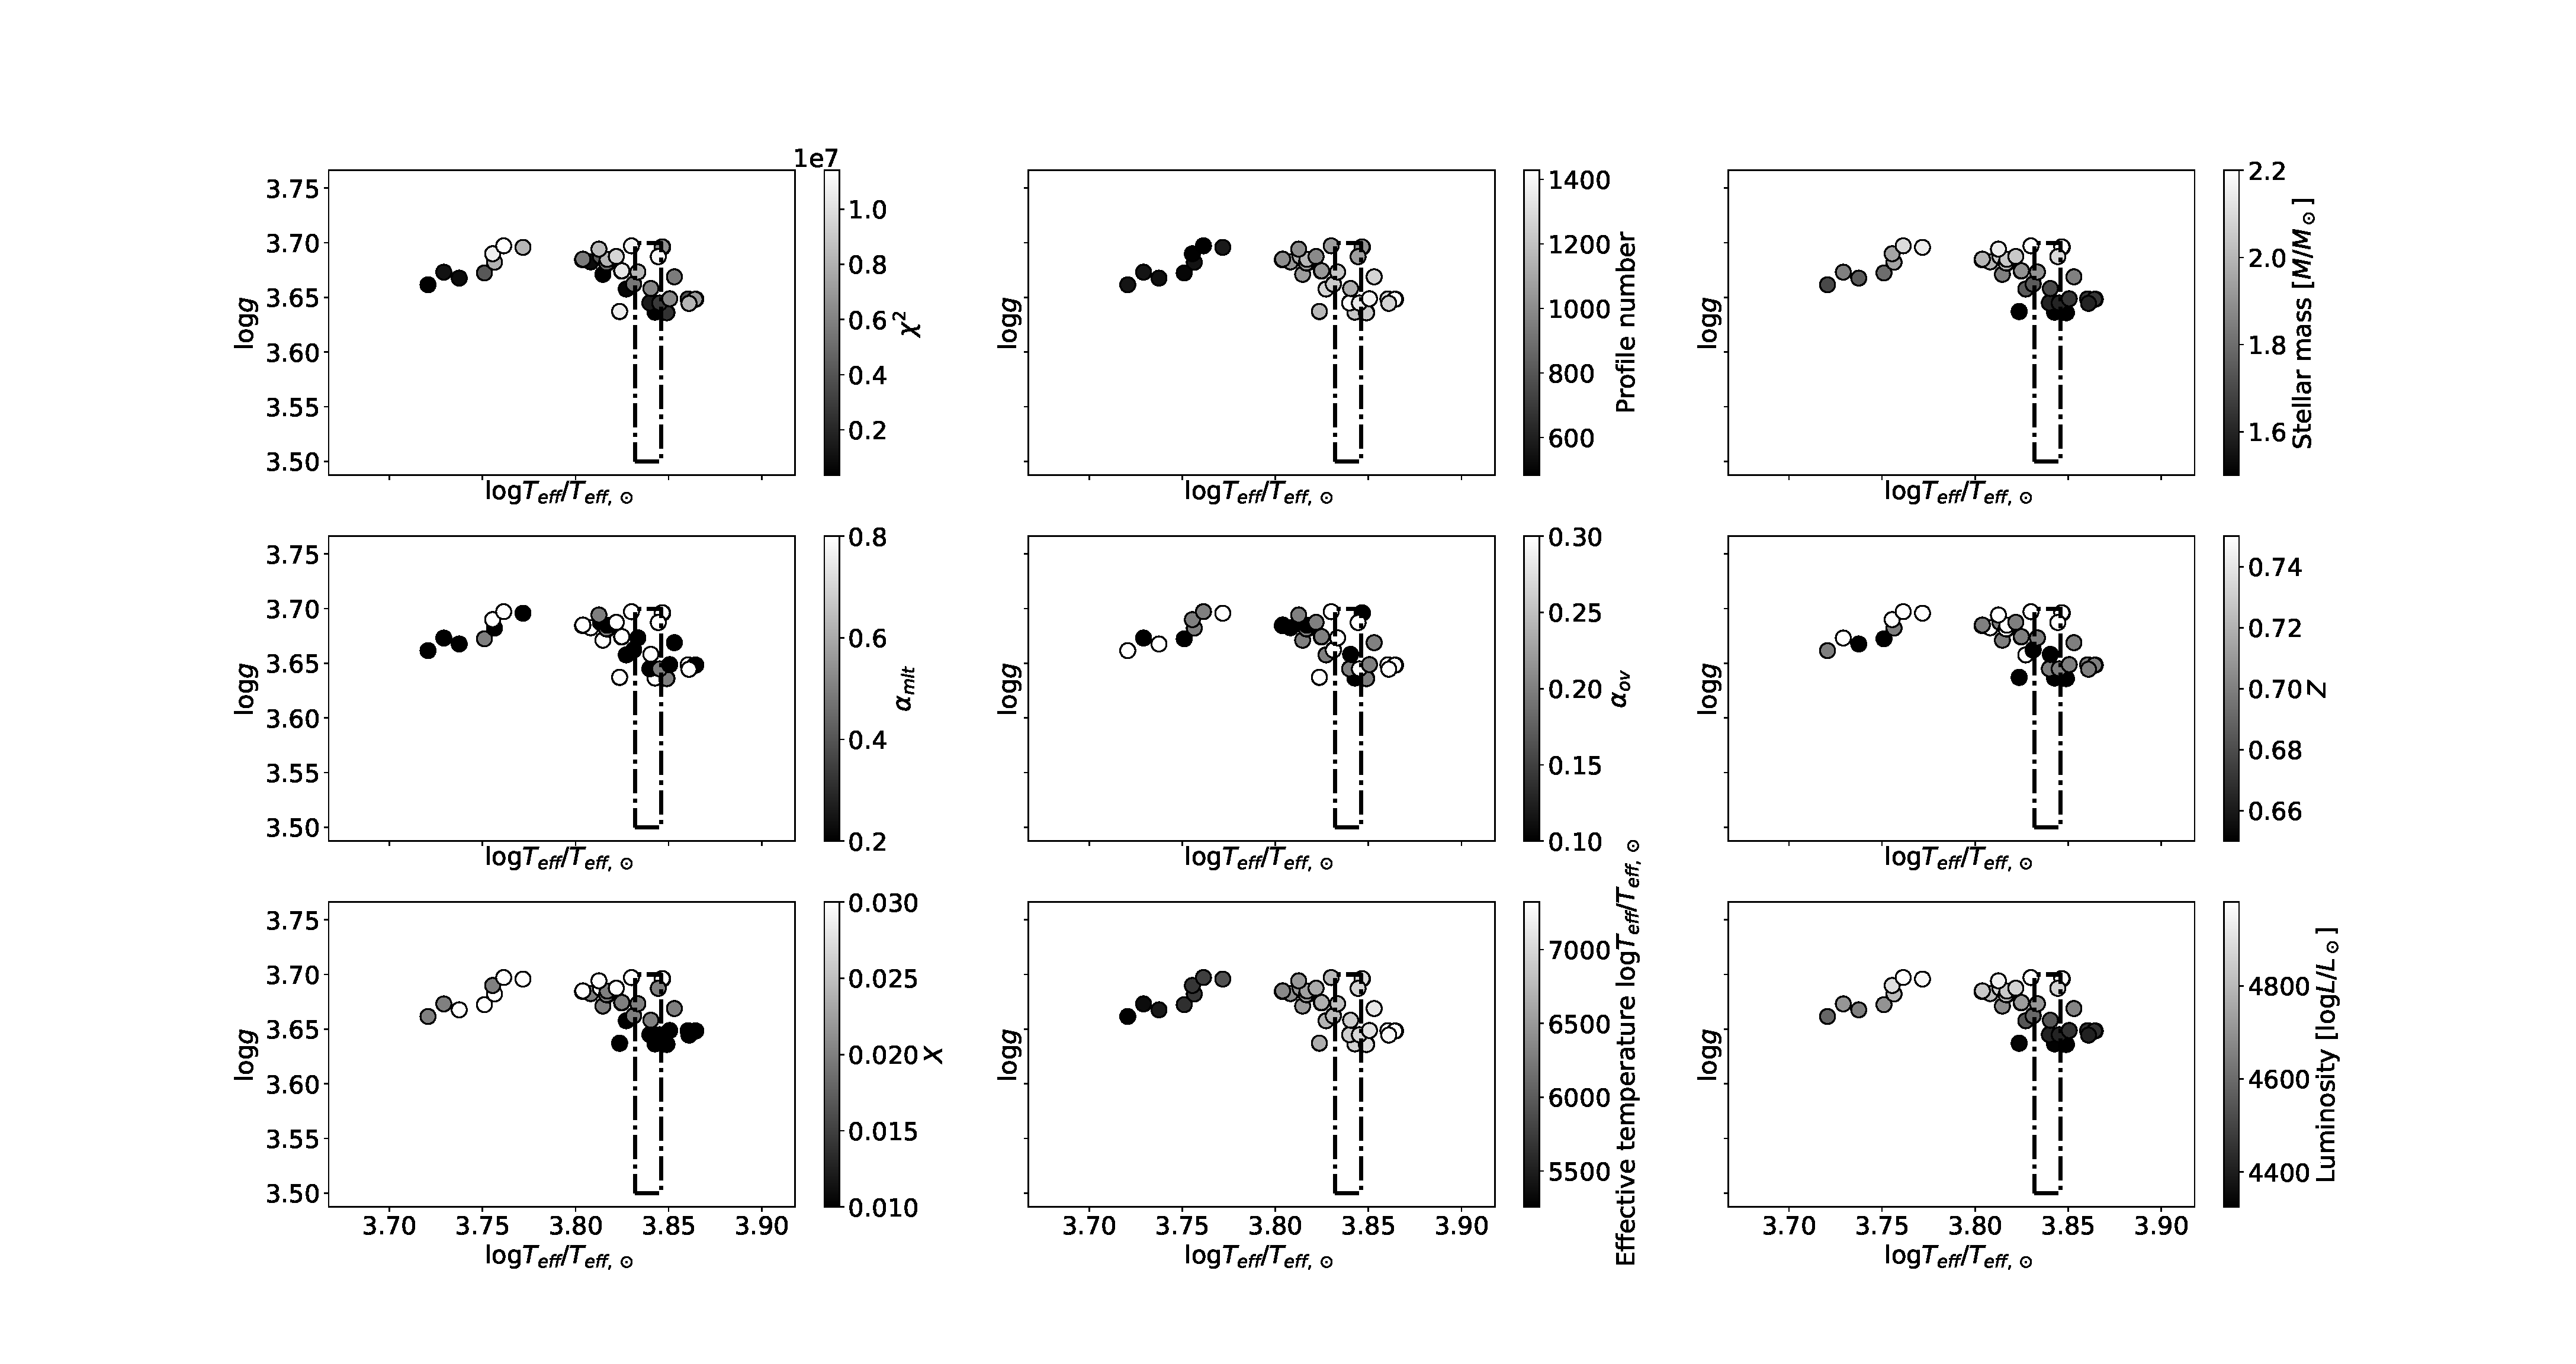
\includegraphics[width=1\textwidth]{scatter_all_v2.eps}
	\makebox[\textwidth][c]{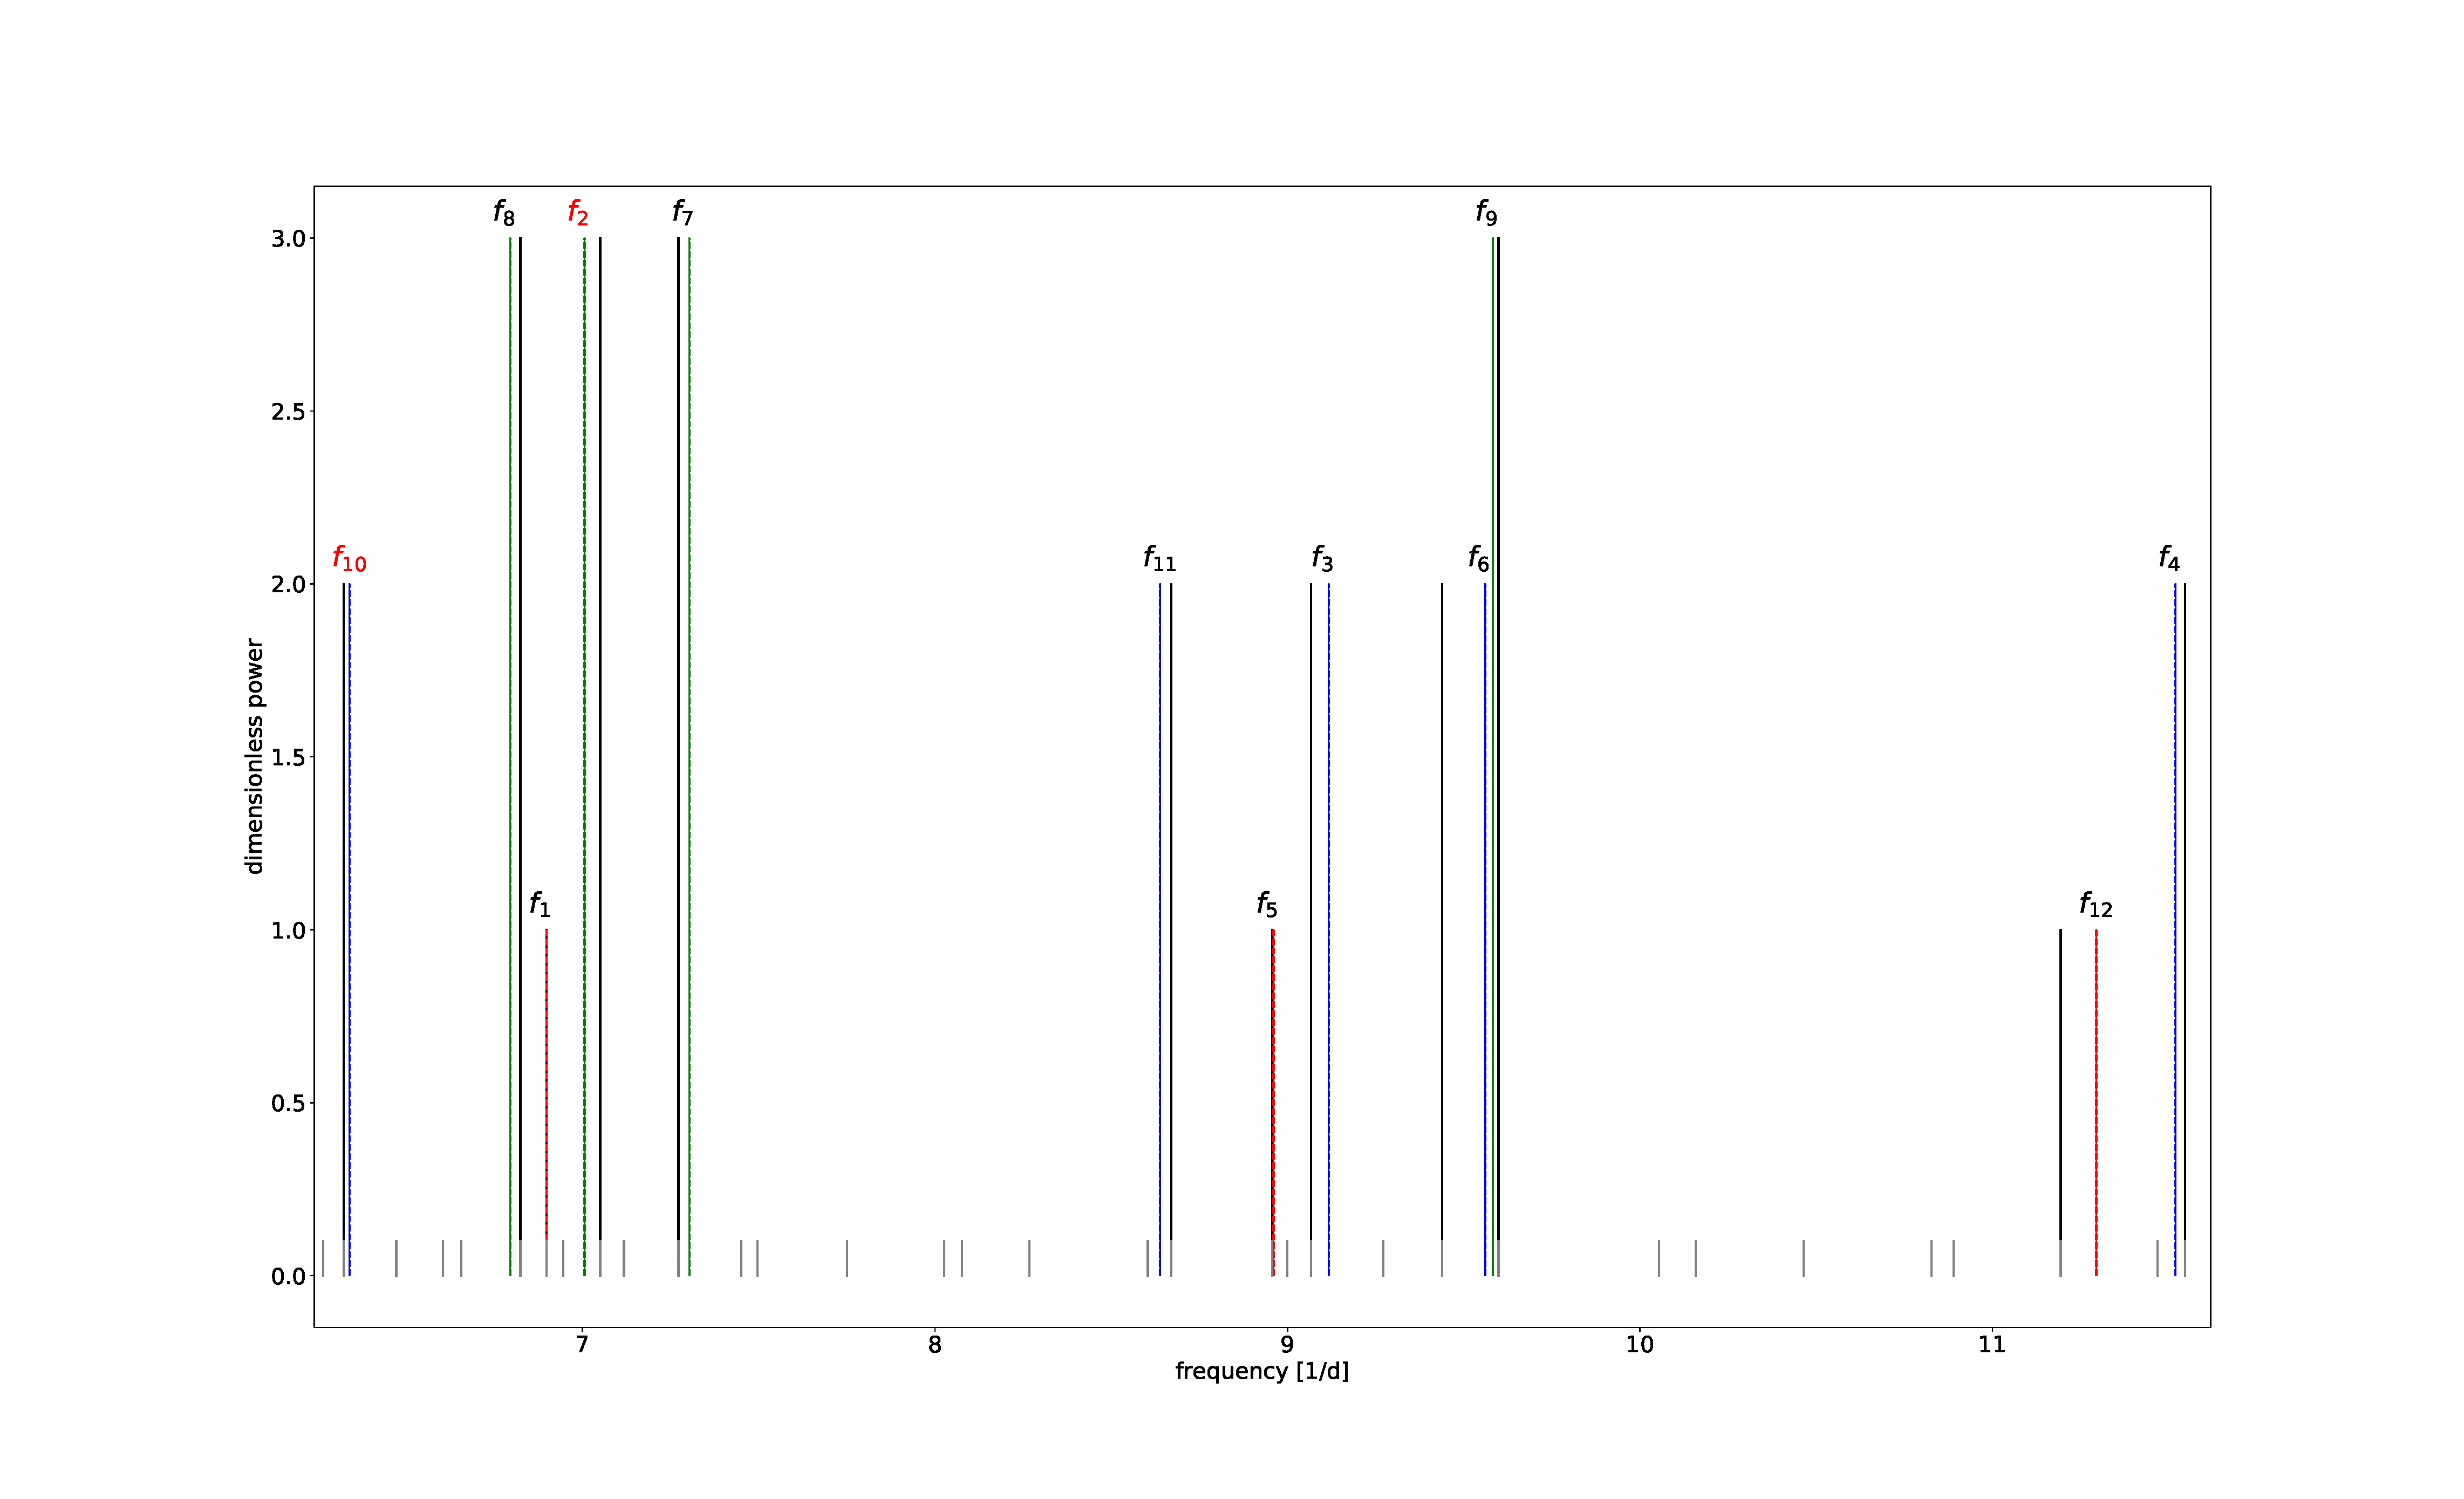
\includegraphics[width=1.2\textwidth]{frequency_fit.eps}}%
	\caption{Frequency fit for $M=1.65$\msun, $X=0.70$, $Y=0.01$, $\alpha_{mlt} = 0.5$, $\alpha_{ov} = 0.3$. Color coding as \figref{freqfitbest}. }
	\label{freqfit}
\end{figure}
\begin{figure}[htbp]
	\centering
	%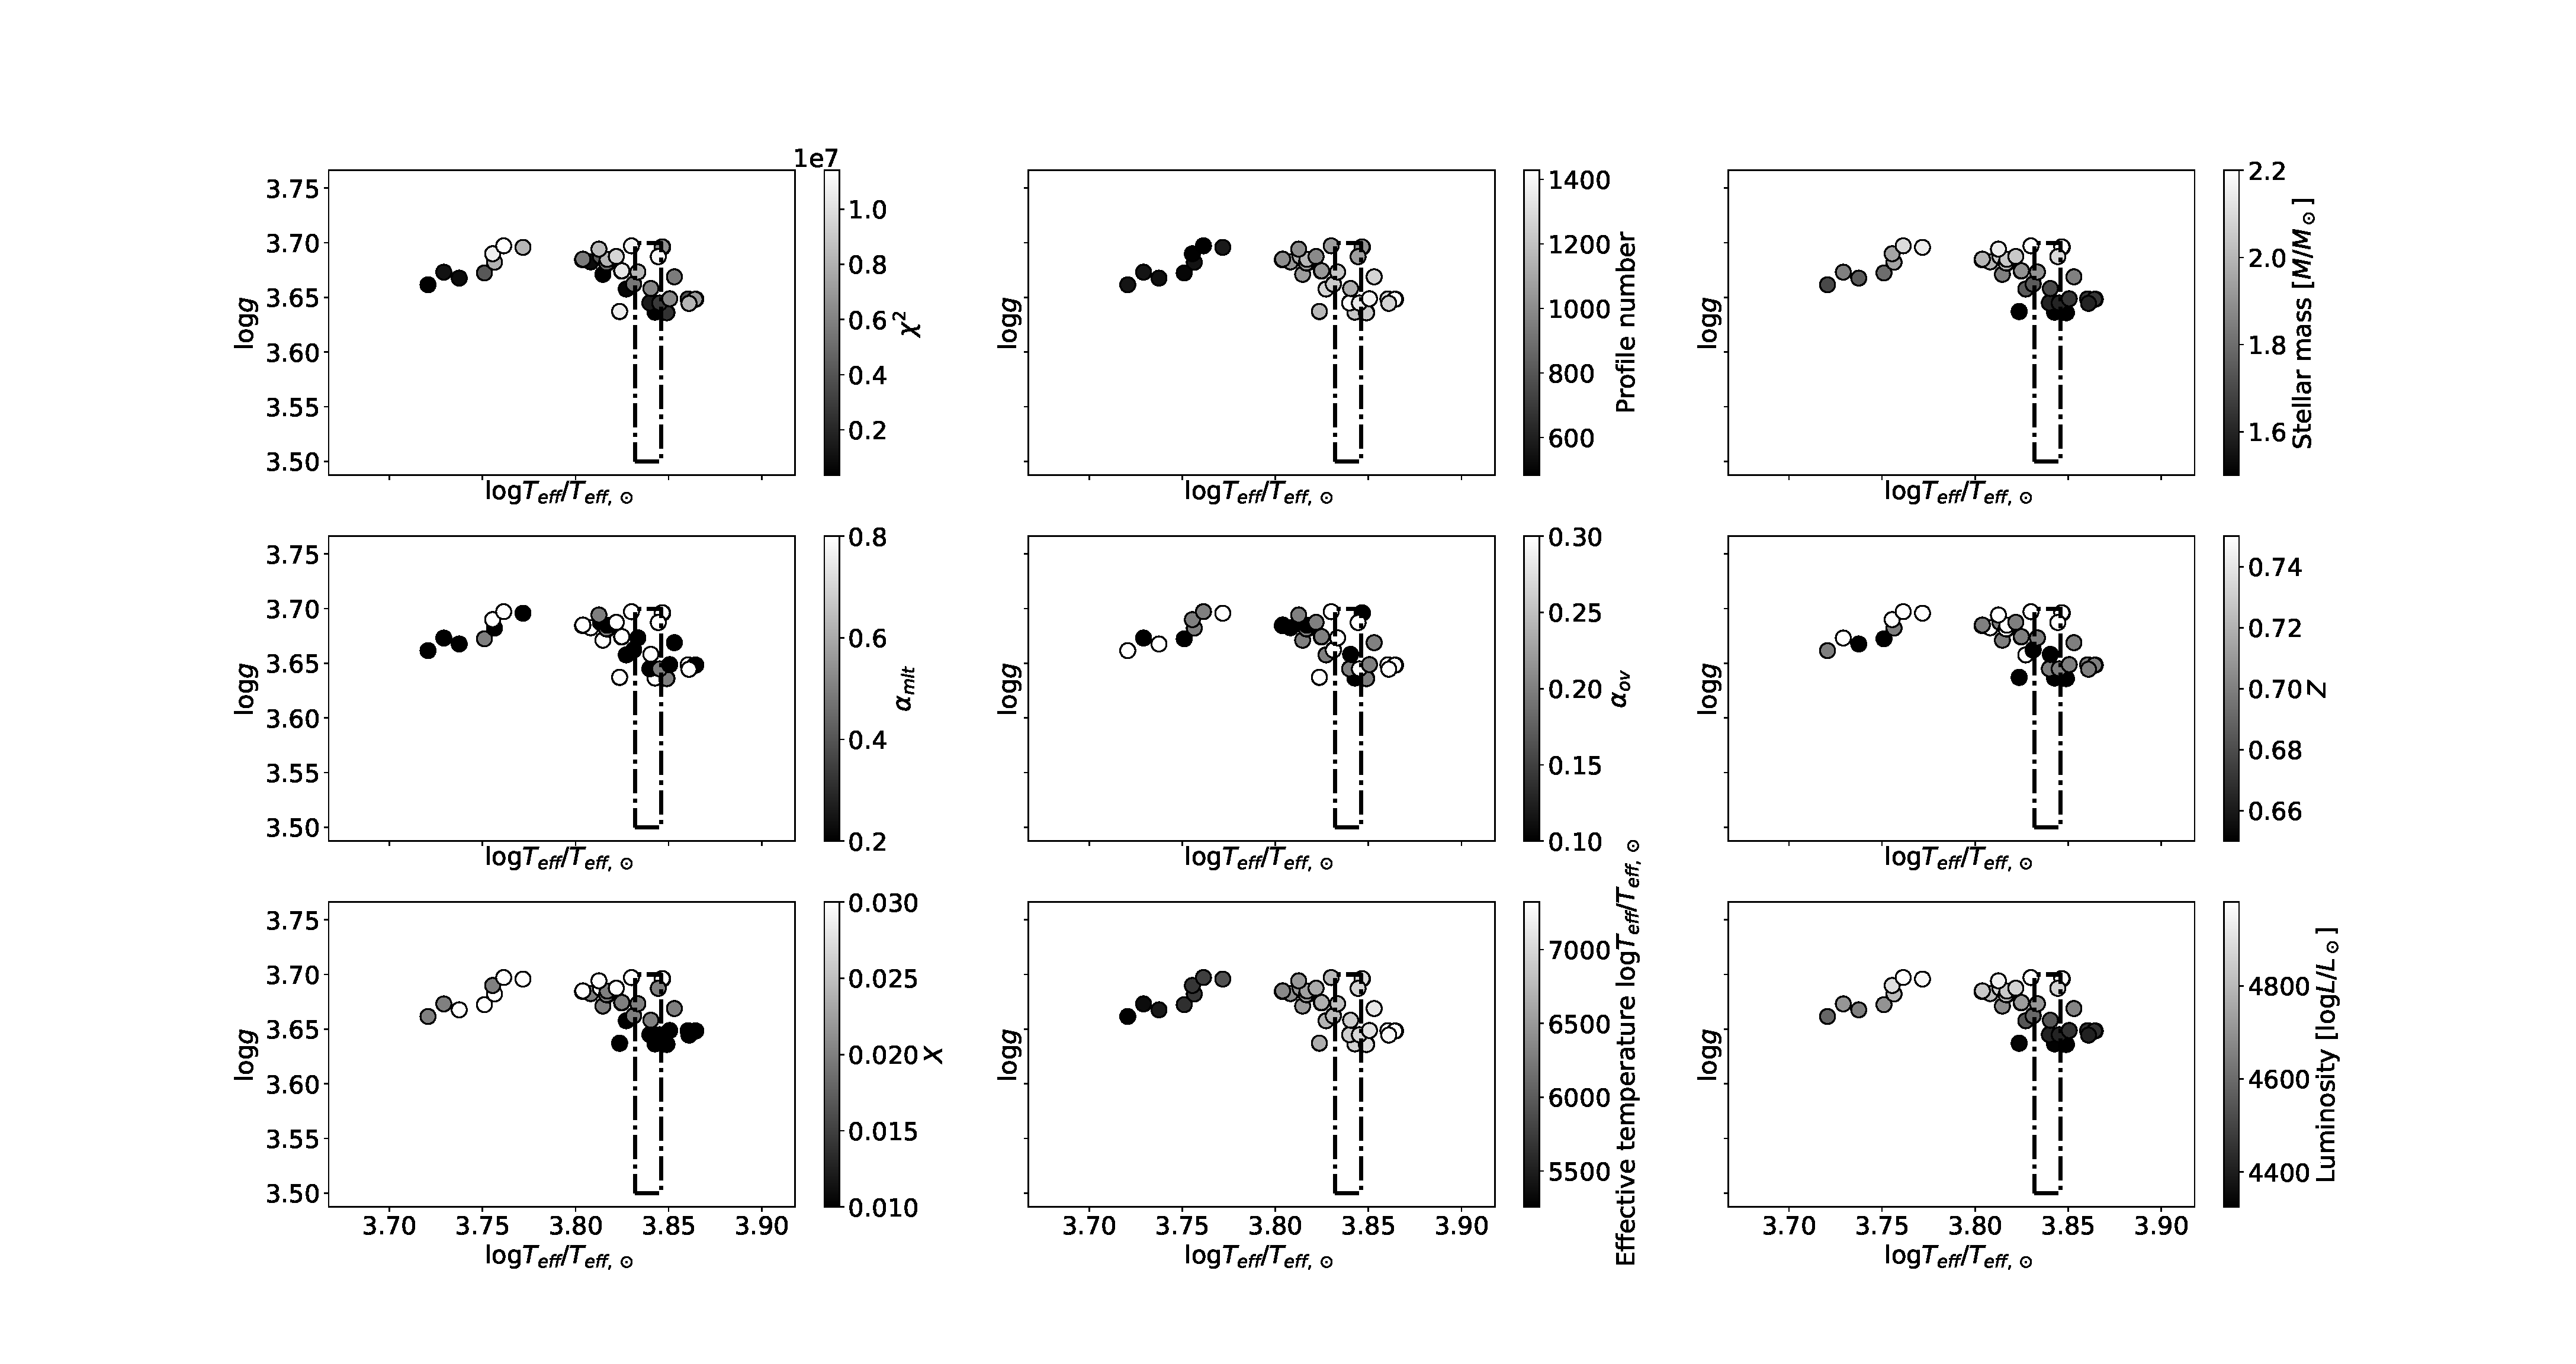
\includegraphics[width=1\textwidth]{scatter_all_v2.eps}
	\makebox[\textwidth][c]{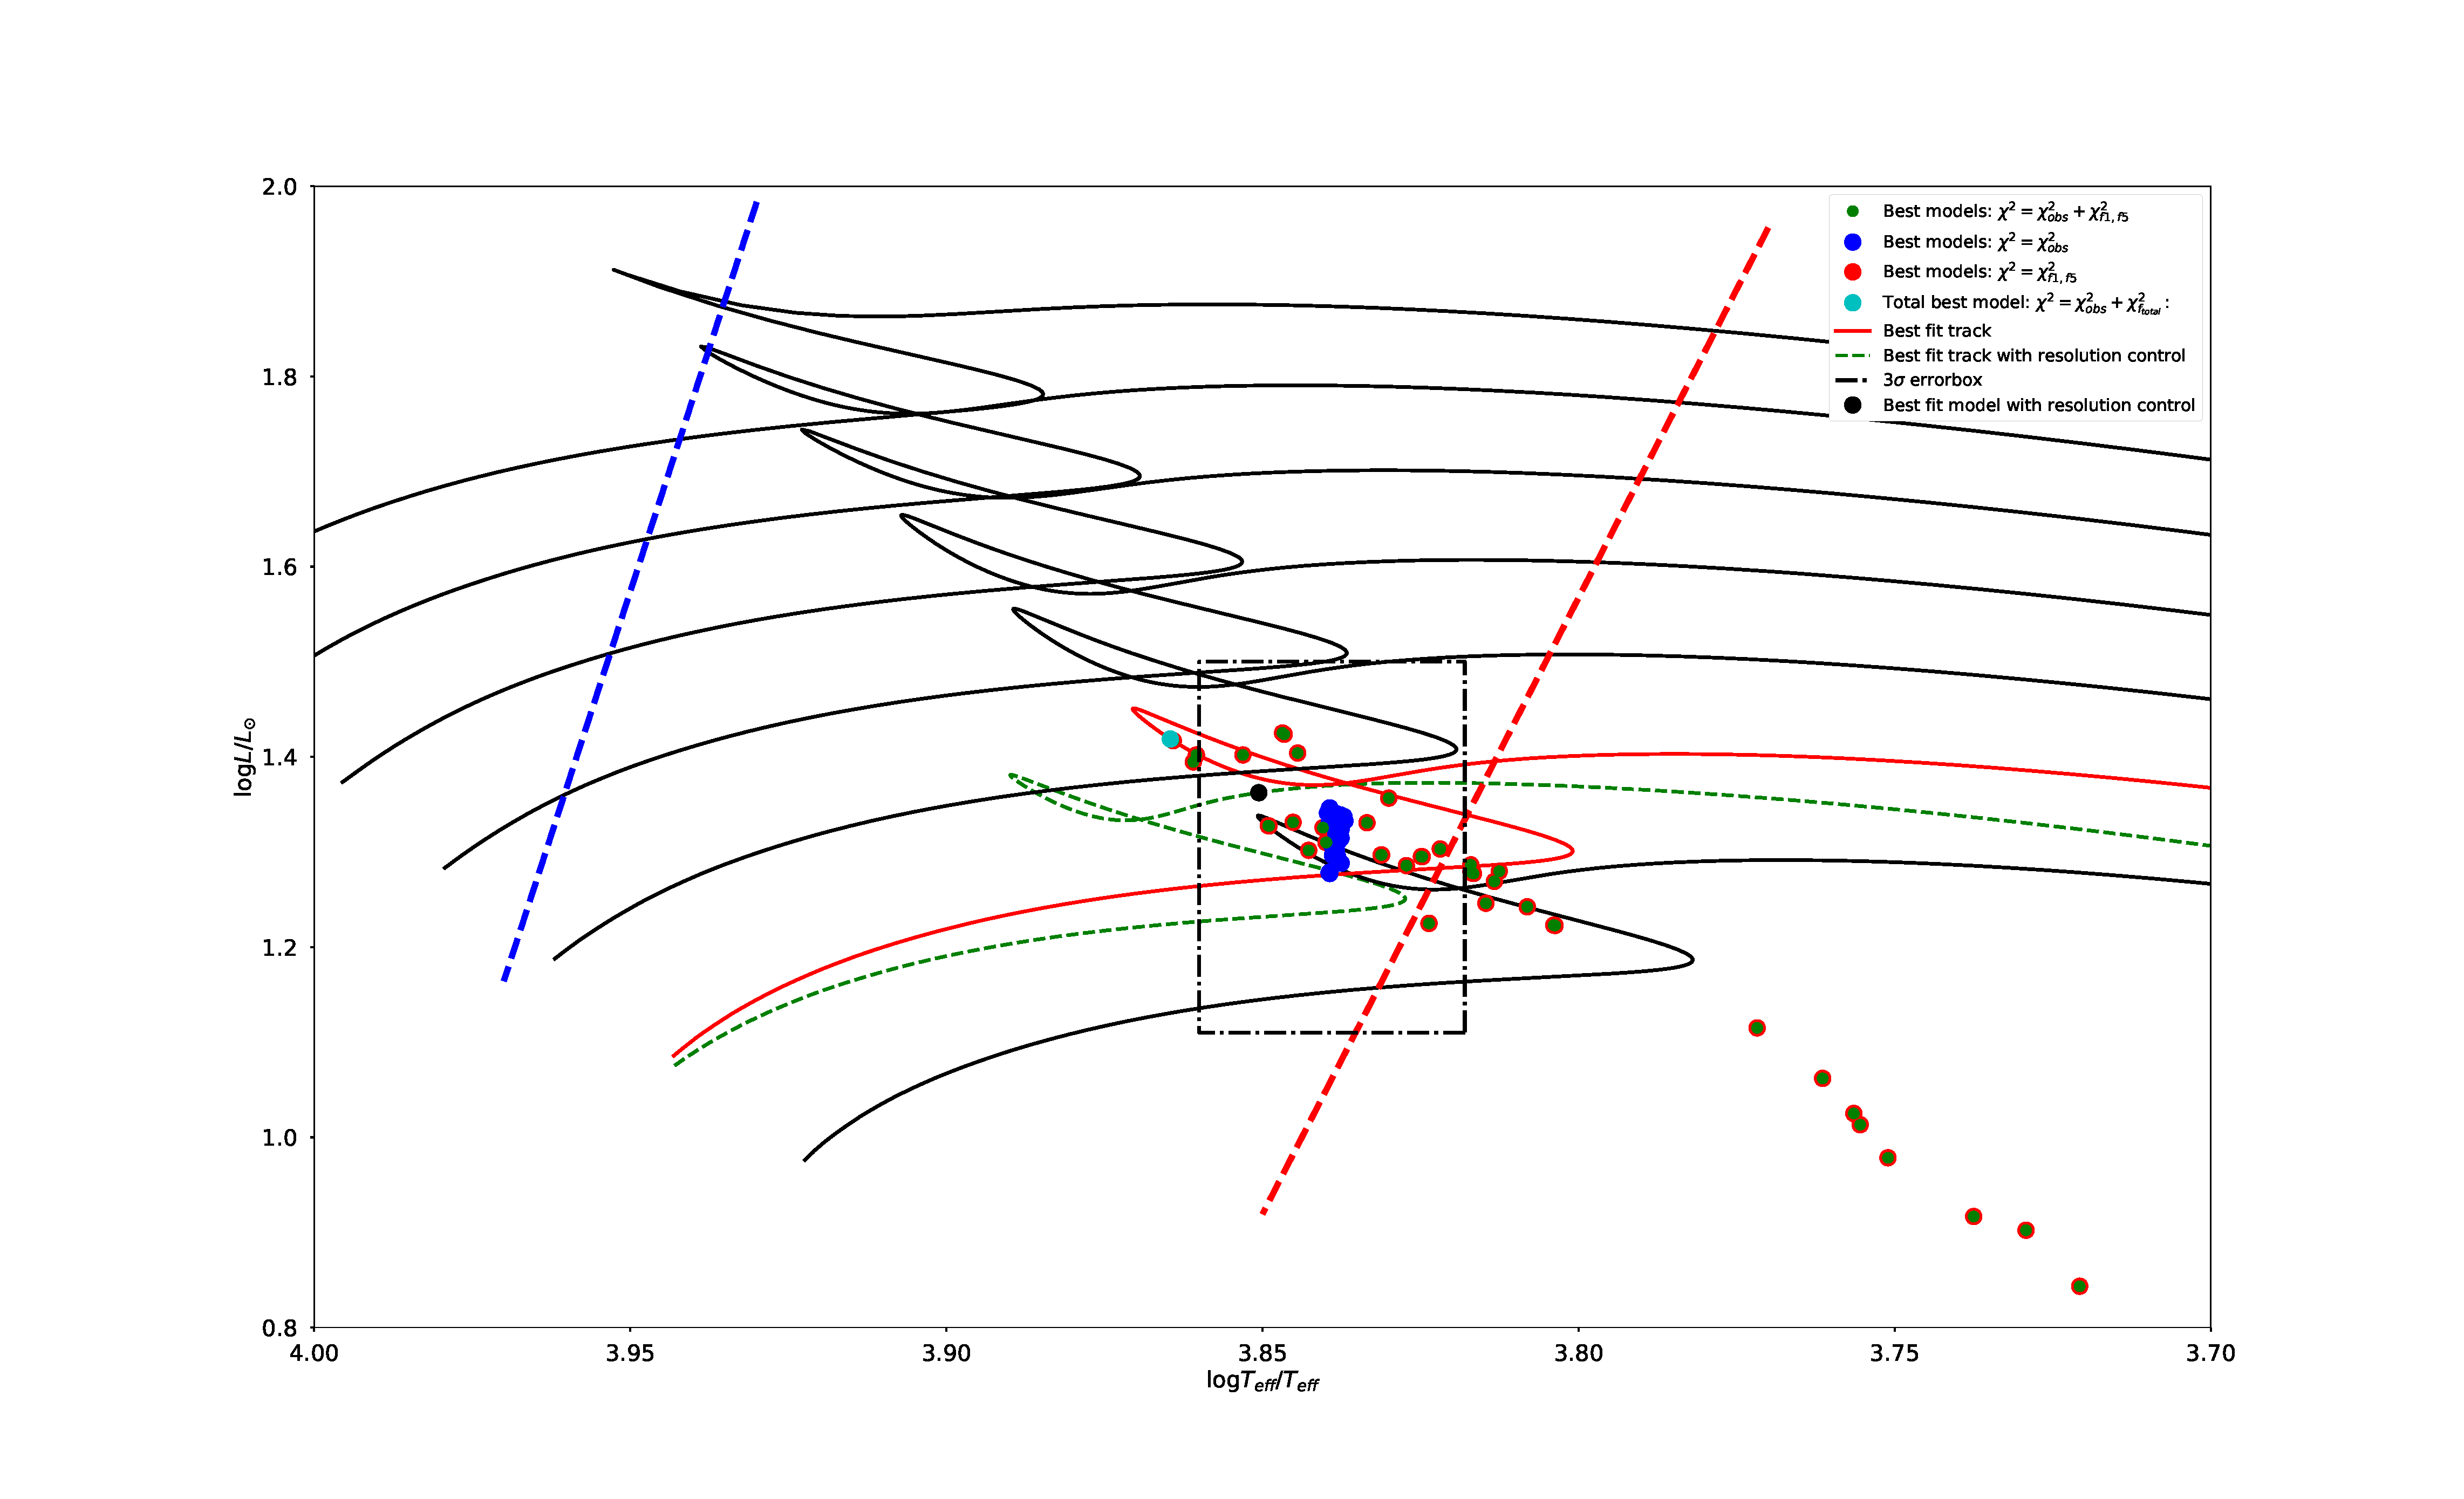
\includegraphics[width=1.2\textwidth]{final_hrd_44tau_lum1.eps}}%
	\caption{HRD where the best model is estimated to be $M=1.65$\msun, $X=0.70$, $Y=0.01$, $\alpha_{mlt} = 0.5$, $alpha_{ov} = 0.3$.}
	\label{hrd44old}
\end{figure}

\section{HD 187547}

On the contrary to 44 Tau, no modes are well enough determined to use an initial constraint for the models of this star. Instead of fitting the frequencies it is therefore more favourable to fit the large frequency separation, now defined as

\begin{equation}
    \Delta\nu = \nu_{n+1} - \nu_{n},
\end{equation}

\noindent the frequency difference between two ($l$=0) consecutive frequencies with same $l$\footnote{This is not the same frequency separation as in \eqref{deltanu}. Thjs does not require $n \ll l$ and is not necessarily asymptotic. Therefore, the values calculated for $\Delta f$ are not to be compared with $\Delta \nu$. For \citet{antoci2011excitation} these were assumed to be the same as the HD 187547 was assumed to have solar-like oscillations in this region where the asymptotic relation applies.}.  The \chis can now be calculated using the observed large frequency separation of $3.5d^{-1}$ AND $7d^{-1}$ \citep{antoci2014role}. Results are shown shown in \tabref{tab:superstar}.



For modes higher than $l$=0, calculating the \chis for HD 187547 is more elaborate than for 44 Tau, since it is based on the large frequency separation. When $l>0$ , the frequency separation depends significantly on the mixed modes and radial order. Therefore, this part is beyond the scope of this work. 

\subsection{Results}
The best models for the two different HD 1987547 runs can be seen in \tabref{bestchisuper}. The best model of the respective \chis is marked with red. For $\Delta \nu=3.5 d^{-1}$ the best model based on $\chi_{tot}^2$ with a theoretical $\Delta f = 3.5672$. Only looking at the $\chi_{sep}^2$, the best model will be slightly shifted, and obtain a significantly higher $\chi_{tot}^2=1254$. This is indicates that if the large frequency separation fits well, the observable parameters will not fit nearly as well. The model with the best $\chi_{obs}^2$ does indeed have a $\Delta f \approx 6d^{-1}$, significantly higher than $3.5d^{-1}$. This strengthens the suspicion that $3.5 d^{-1}$ is too low to match the observed parameters. This can also be seen on \figref{finalsuper}, as the best total track is forced outside the bounds of the instability strip.  From the placement of the 5\% best models it can be seen that the separation is closely related to the evolutionary stage (as they tend to line up along the same stage of the tracks. ) There is not overlap between the models for $\chi_{sep}^2$ and $\chi_{obs}^2$. The best combined modes therefore match the luminosity relatively, but is not within the errrorbox of the \teff, or \lum. The best model (marked in black) does place HD 187547 on the main-sequence, however to the right of the red edge, pushing it outside of the instability strip. 
\begin{figure}[htbp]
	\centering
	\makebox[\textwidth][c]{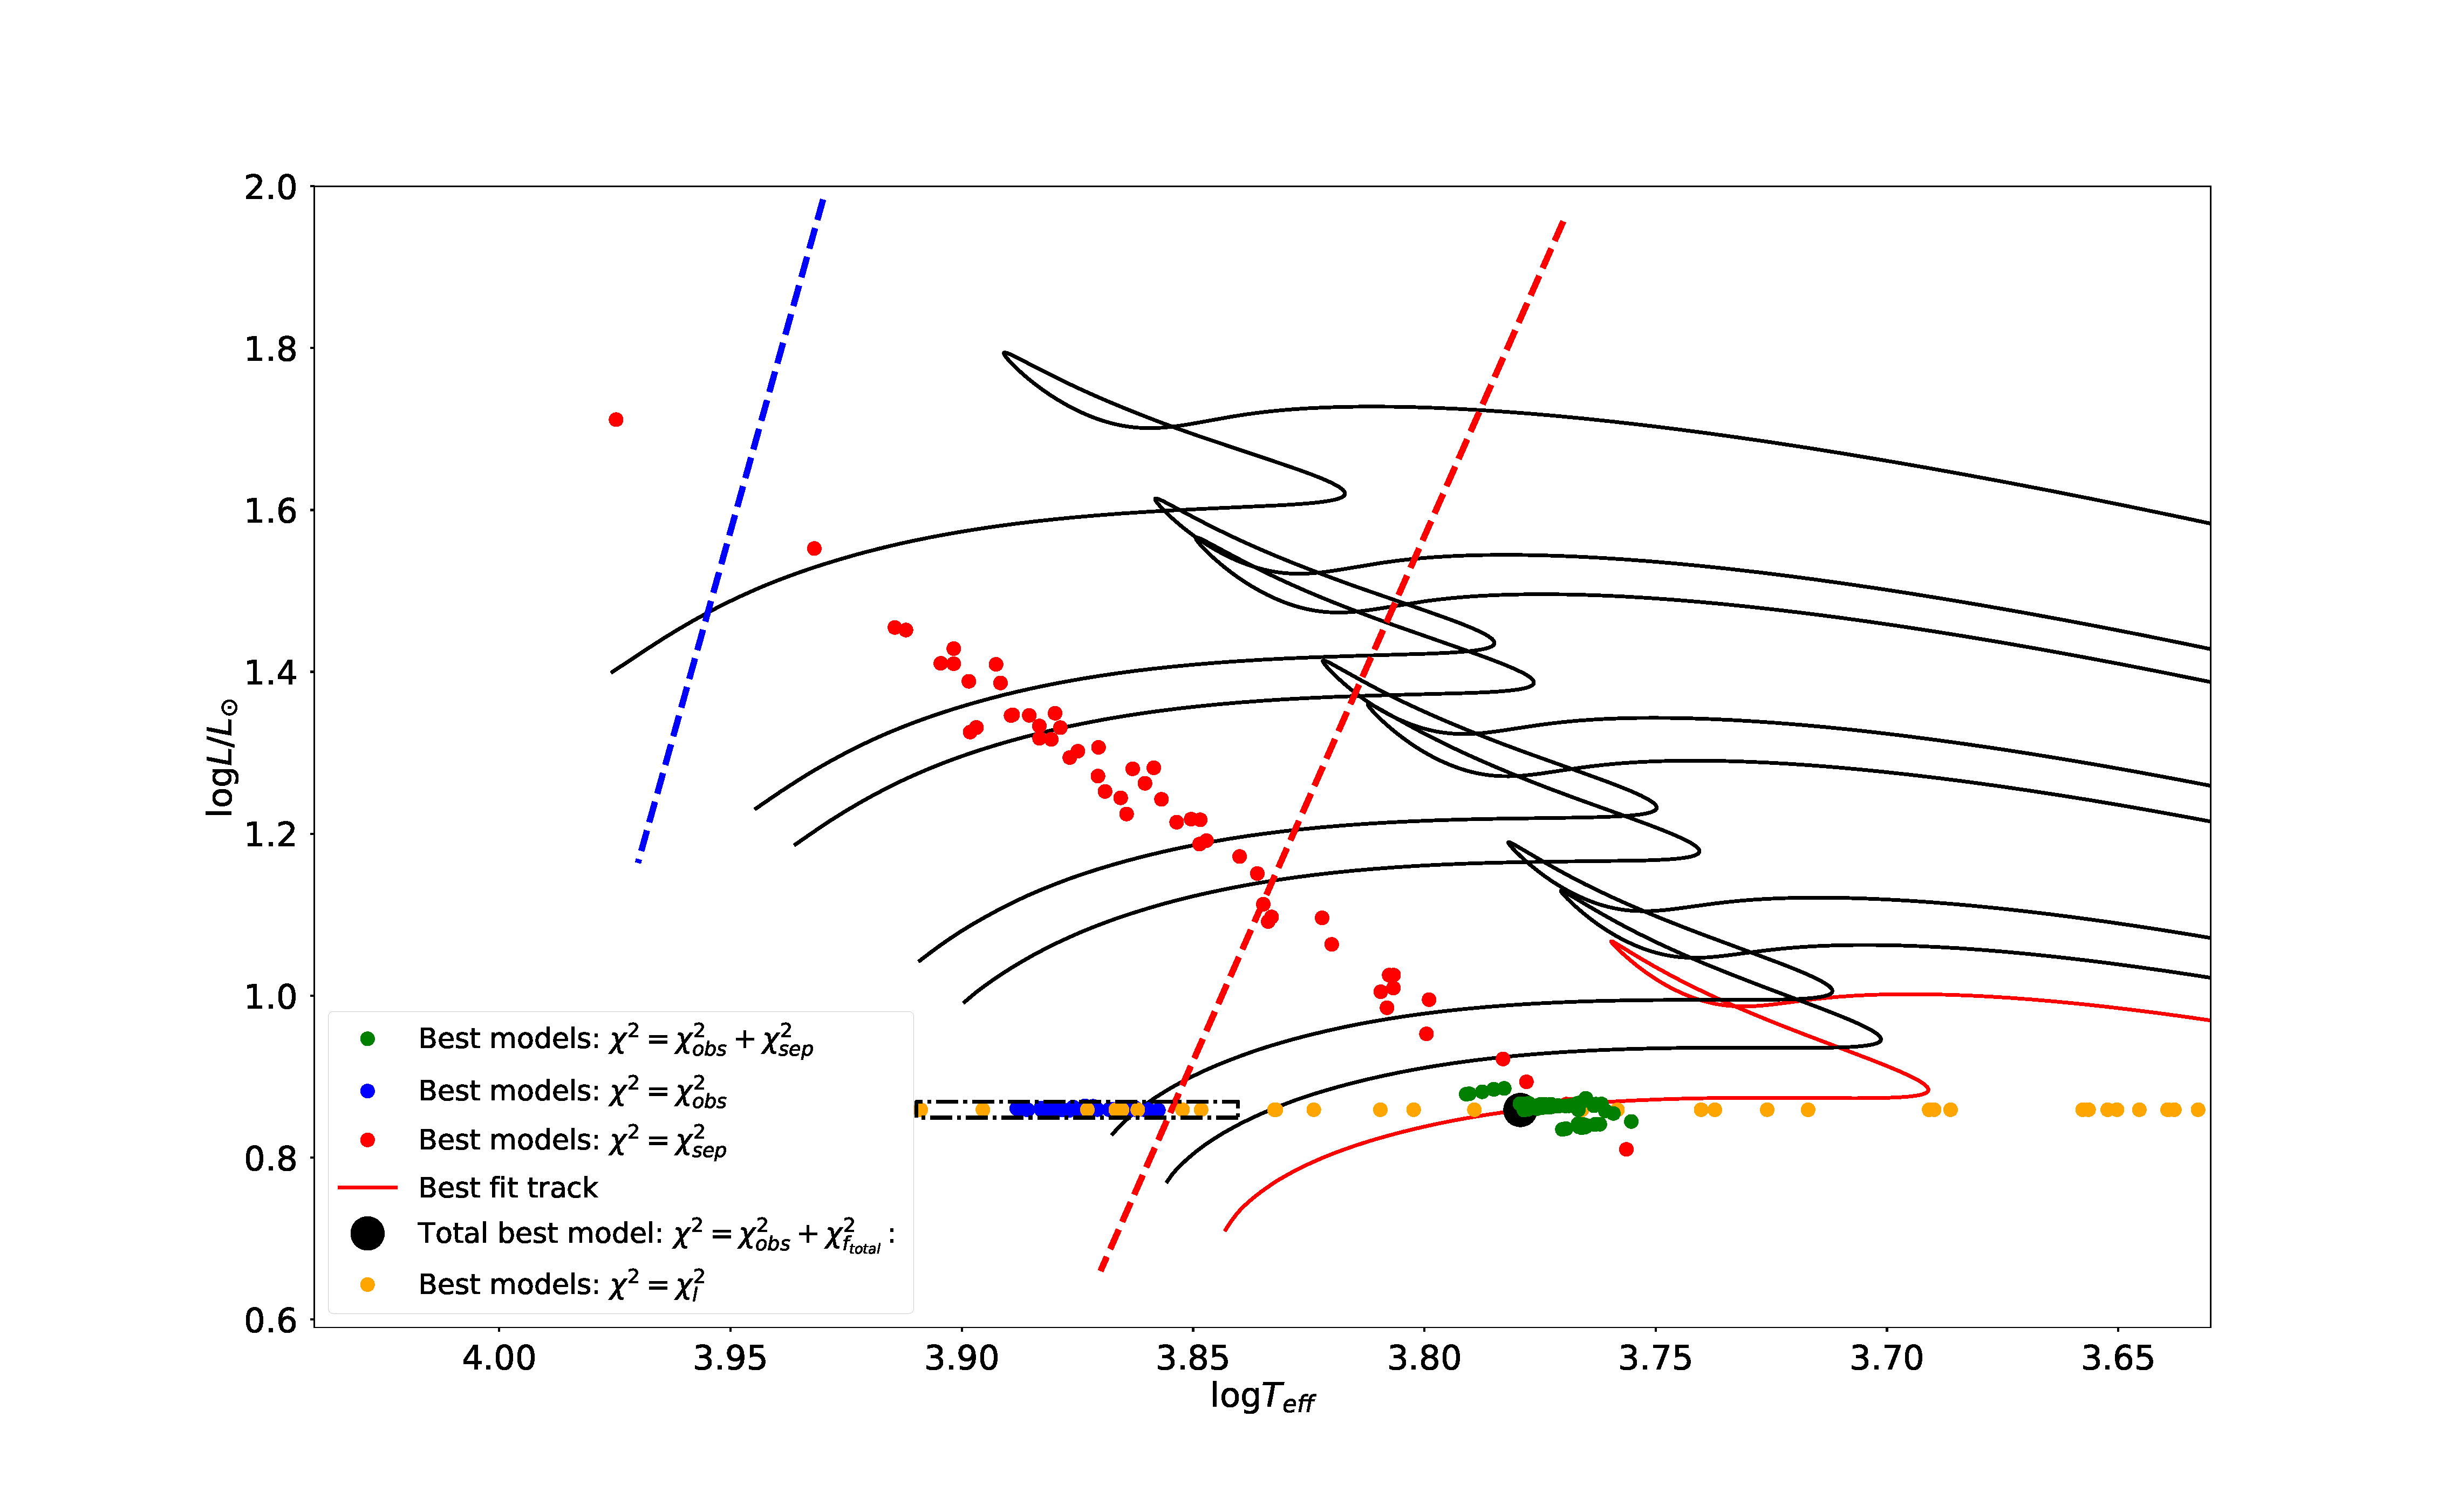
\includegraphics[width=1.2\textwidth]{finalsuperstar_35.eps}}%
	\caption{HRD for HD 187537. The tracks for which $\chi_{tot}^2$ icds lowest is marked with red. The black tracks have the same parameter combinations as the best track but with masses varying from $M=1.55$ to $M=2.2$ \msun. The red dots are the plotted 5\% best models based on the \chis from the separation only ($\chi_{sep}^2$).  Here, $\Delta \nu = 7^d{-1}$ The blue points are the best 5\% for observed parameters $\chi_{obs}$, and the green dots for the combined $\chi_{tot}^2$. The orange dots indicates best models for \chis calculated based on \lum. Three sigma observed uncertainties are marked with a black dashed line as an errorbox. The instability strip is marked with the blue and red edges from \citet{murphy2019gaia}.}
	\label{finalsuper}
\end{figure}
%Large frequency separation plays a big role for the \chis, as it is a strong indicator of the evolutionary stage. The frequency separation as a function of evolution is shown on \figref{plotfreqsastime} for te best model.  As mentioned in \chapref{chap:asteroseismology}, the large frequency separation only behaves asymptotically for $n \ll l$. This is somewhat accomplished as the frequency ranges for all models is chosen to be $45-80d^{-1}$.

\begin{sidewaystable}
%\begin{table}[]
	\caption{Best models for superstar with the two different $\Delta \nu$ . The \chis are calculated by comparing theoretical parameters with the observational parameters are $\log T_{eff} = 3.875 \pm 0.011$, $\logg = 3.9 \pm 0.2 $ and \lum$=0.859 \pm 0.003$. The best \chis value for the different parts of the \chis is marked in red. }
	\label{bestchisuper}
	\begin{tabular}{lllllllllllllll}
		\toprule
		profile & M[$M_\odot$] & X & Z & $\alpha_{mlt}$ & $\alpha_{ov}$ & \teff & \logg & \lum & Age [Gyr]& $\chi_{tot}^2$ & $\chi_{obs}^2$ & $\chi_{sep}^2$ & $\Delta f_{theo}$&$\Delta\nu_{obs} [d^{-1}]$\\
		\midrule
		  1144  &  1.50  & 0.65   & 0.03   & 0.2   & 0.3  & 3.7793 & 3.8257  & 0.8587 &2.1183 & \textcolor{red}{70.399}  & 68.595  & 1.8049 & 3.5672 &3.5   \\
		  964  &  1.50  & 0.75   & 0.01    & 0.8   & 0.2  & 3.8730  & 4.2010  & 0.8586 &  1.2542 &  2728.3 & \textcolor{red}{2.3180}  &  2726.0 & 6.1105 &3.5    \\
	     1128  & 1.75    & 0.75  & 0.02     & 0.2  & 0.2  & 3.8076  & 3.8394 & 1.0254 & 1.8019 & 2605.9  & 2605.9  & \textcolor{red}{$1.2759 \cdot 10^{-9}$}& 3.5000  &  3.5  \\
		  991  &  1.55  &  0.75  & 0.01       & 0.5  & 0.1 &  3.8933  & 4.2949  & 0.8601  & 0.6093   &  \textcolor{red}{6.5110} & 6.4926  & 0.0166  & 6.9932 &7.0 \\
	      964 &  1.50  & 0.75  & 0.01      & 0.8  & 0.2  &  3.8730 & 4.2010   & 0.8586 & 1.2542  &  318.77 &  \textcolor{red}{2.3180,0} &  316.46 &
	      6.1105 &7.0 \\
		  966 &  2.05 & 0.70  & 0.01      & 0.2  & 0.1  &  4.0244 & 4.3283 & 1.4721 &  0.0061   &  35171  & 35171 &   \textcolor{red}{$9.5566 \cdot 10^{-9}$}  & 7.0000 &7.0     \\         
		 \bottomrule
	\end{tabular}
%\end{table}

\end{sidewaystable}
Increasing the large frequency separation to $\Delta \nu = 7d^{-1}$ yields the result shown in \figref{finalsuper7}.

\begin{figure}[htbp]
	\centering
	\makebox[\textwidth][c]{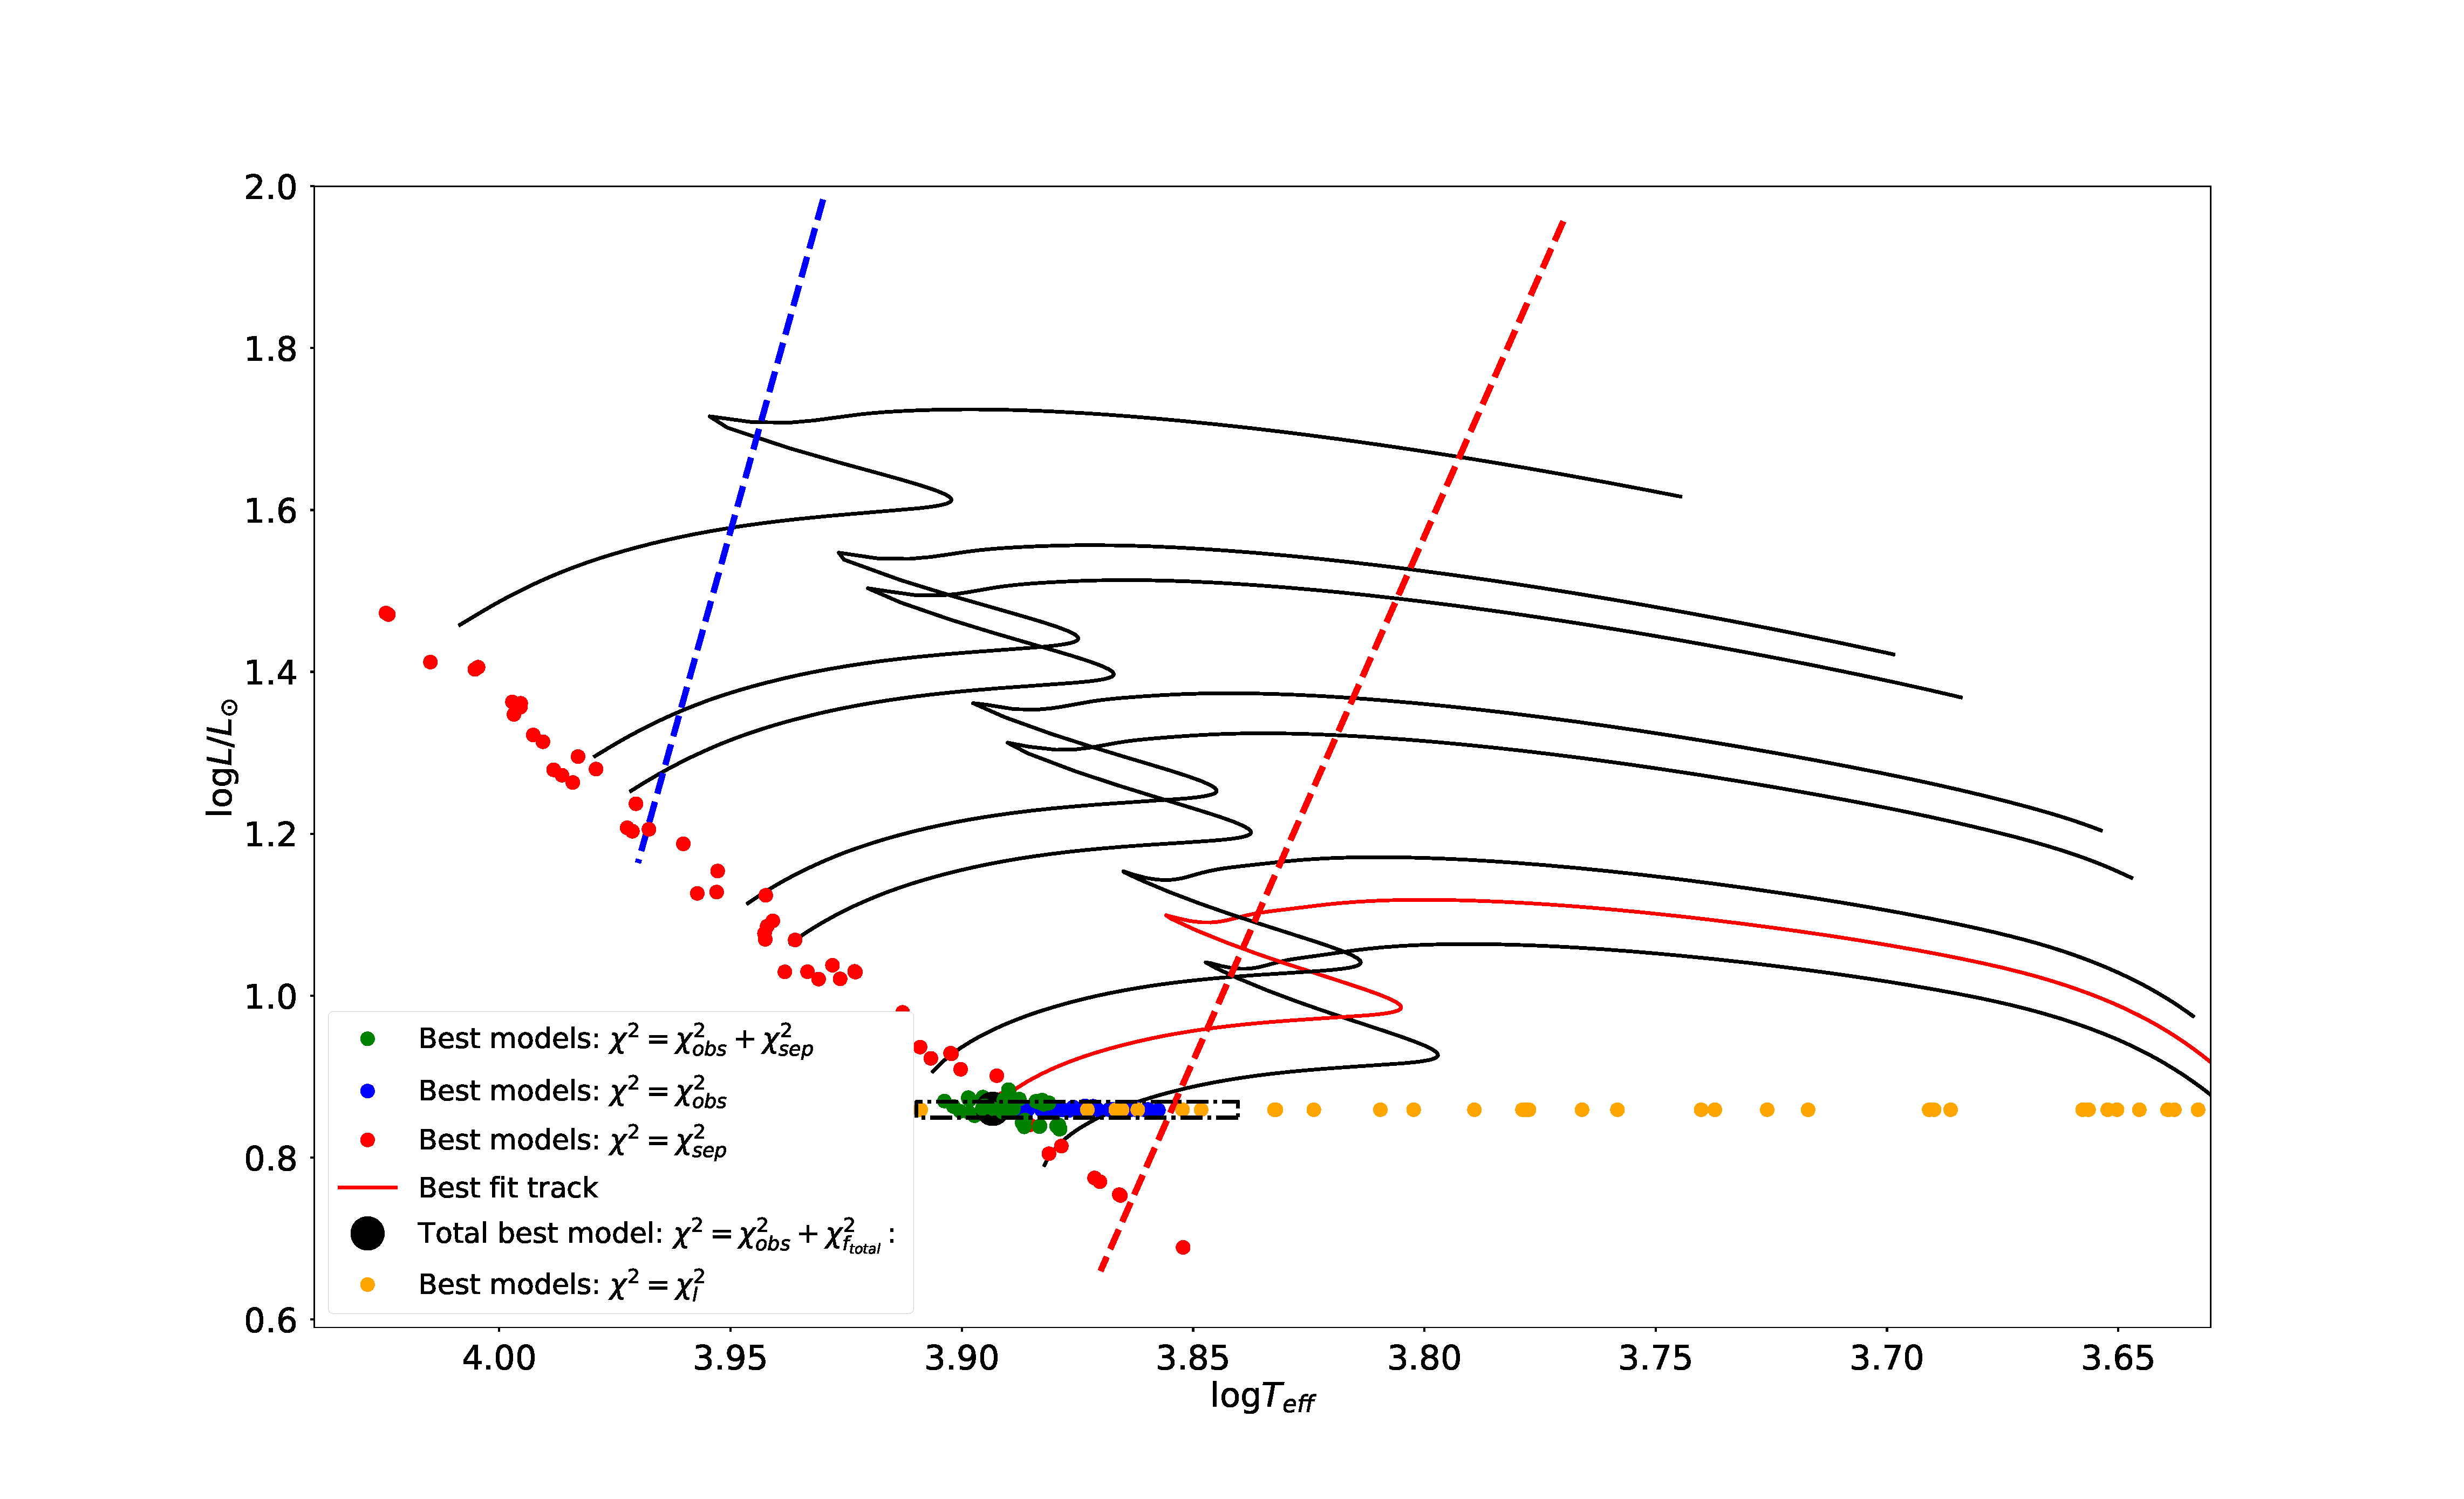
\includegraphics[width=1.2\textwidth]{finalsuperstar_7.eps}}%
	\caption{HR diagram for HD 187537, corresponding to \figref{finalsuper} but with $\Delta \nu = 3.5^{-1}$ . The tracks for which the total \chis is lowest is marked with red. The black tracks have the same parameter combinations as the best track but with masses varying from $M=1.55$ to $M=2.2$ \msun. The red dots are the plotted 5\% best models based on the \chis from the separation only ($\chi_{sep}^2$). The blue points are the best 5\% for observed parameters $\chi_{obs}$, and the green dots for the combined $\chi_{tot}^2$. The orange dots indicates best models for \chis calculated based on \lum. Three sigma observed uncertainties are marked with a black dashed line as an errorbox. The instability strip is marked with the blue and red edges from \citet{murphy2019gaia}.}
	\label{finalsuper7}
\end{figure}


The best track in this case is still on a low mass of $M=1.55$\msun, but is now inside the red edge of the instability strip. This also puts HD 187547 at a stage very early on the MS. There is now an overlap between the best models from separation and the best models for parameters. The $\chi_{ tot}^2$ is lower than for the run with $\Delta \nu = 3.5d^{-1}$, suggesting a better fit. What is to be noted is that the best model for the separation only ($\chi_{sep}$) is smallest on a track with a significantly higher mass $M=2.05\msun$.  The $\chi_{tot}^2$ however, is much larger. 

If HD 187547 is on the PMS we would expect features from different metallic lines and dust to appear in the spectrum, however no so observations indicate that this should be the case. As mentioned, the PMS tracks in \texttt{MESA} made in this work should not be trusted for  the purpose of asteroseismic modeling, since the are all products of the same relaxed pre-calculated PMS model. Therefore, the results are forced on to the MS by making a cutoff at profile 900. This is a rough cutoff since profile 900 on one tracks is not necessarily an indication of the same stage for the same profile on another track. This cutoff is marked with a black vertical dashed line on \figref{plotfreqsastime}. The frequency separation $\Delta f$ is shown on \figref{plotfreqsastime}. It can be seen that the large frequency separation decreases somewhat linearly on the MS, until reaching the post-MS phases. The model cutoff in this case (best model for HD 187547) excludes only models on the PMS, yet also includes some models that should not be included. Therefore, this cutoff method should be reconsidered. 

\begin{figure}[htbp]
	\centering
	\makebox[\textwidth][c]{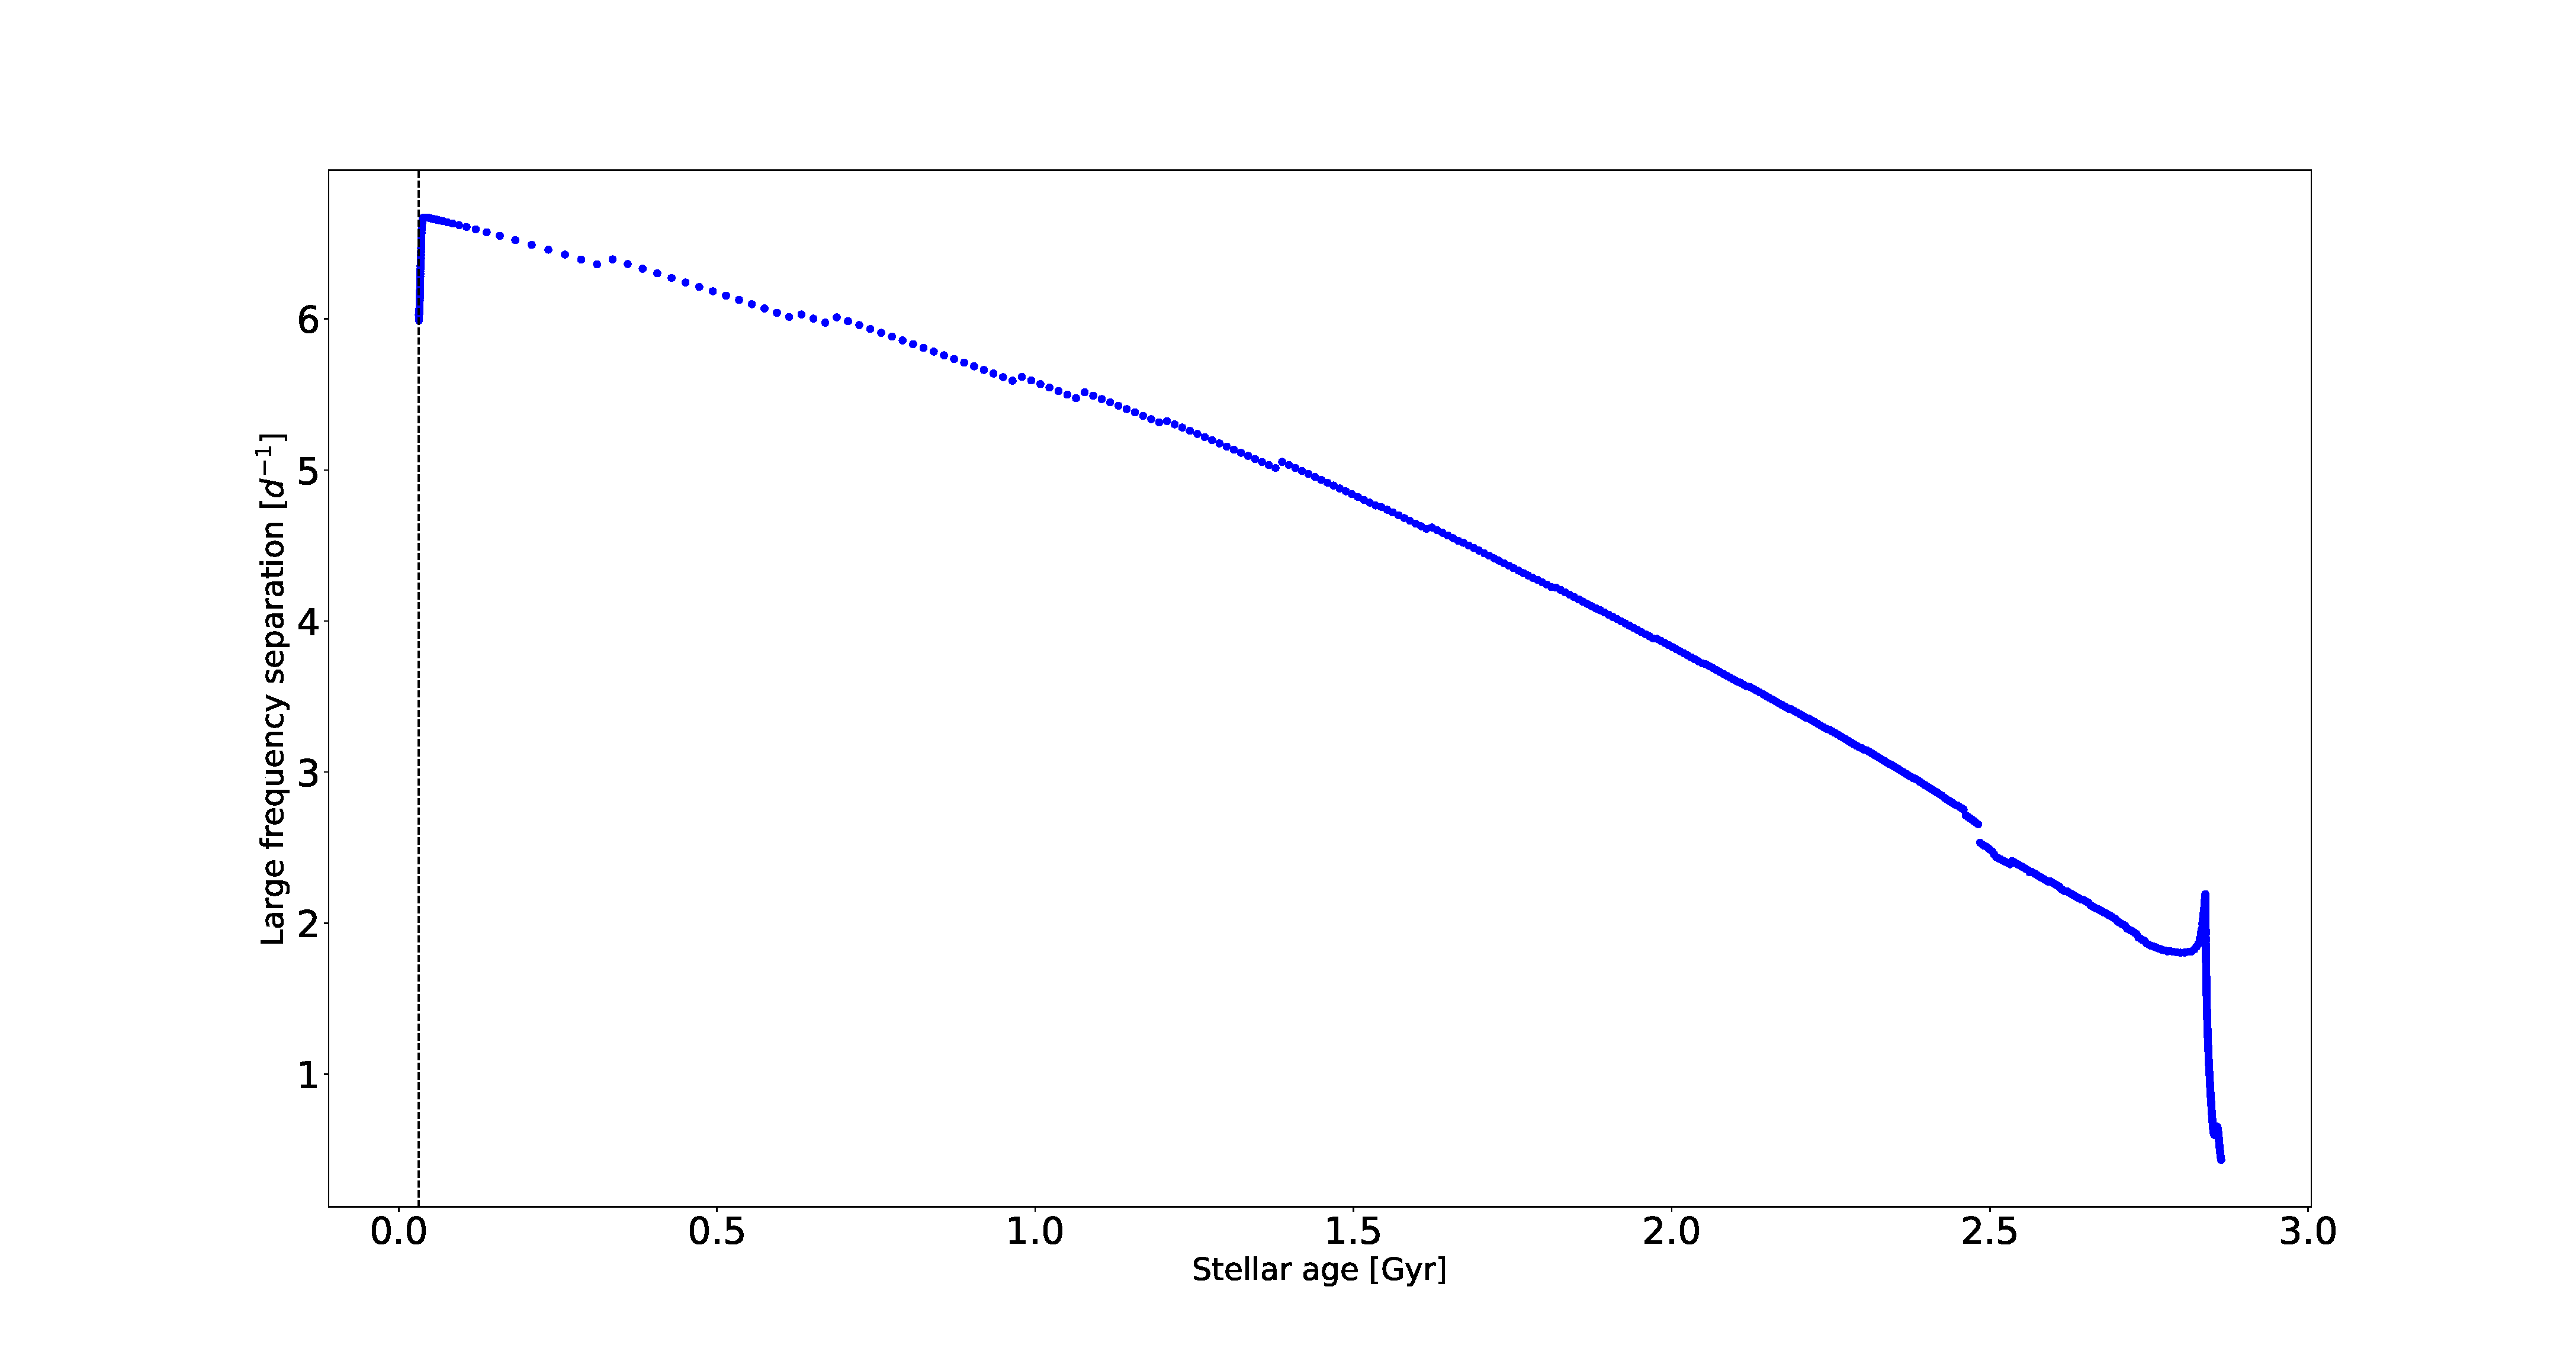
\includegraphics[width=1.2\textwidth]{freqsvsevol.eps}}%
	\caption{Large frequency separation as a function of evolution for a track wit h$M=1.5$\msun, $X=0.65$, $Z=0.03$, $\alpha_{mlt}=0.2$ and $\alpha_{ov}=0.3$.}
	\label{plotfreqsastime}
\end{figure}

 A more secure way do it would be to evaluate the helium content in the core and set a limit for the gradient (i.e., defining the ms at a certain limit for an increase in helium in the core). This would however require an individual assessment of each track and is therefore beyond the scope of this work. 

%The very small luminosity measured observationally could be explained if it is still in a vary early stage on the ms. Then we would expect $\delta \nu$ to be significantly larger than $3.5d^(-1)$, more like $7d^(-1)$ from Bedding. However, since the pre-ms tracks made in \texttt{MESA} in this work are not made for modeling purposes, the earlier stages of the ms might be affected as well (due to relaxation issues etc.). 
%For the small frequency separation, the results seems more reliable as the 5\% best models for separation and observations has some overlap, which is not the case for the $\delta \nu = 7$. 
%This could be due to several things: 1) The models are simply not trustworthy at these early stages due to insufficient pre-ms tracks. 2) From the resolution evaluation discussed in \secref{sec:resolution}, it was shown that models have smaller resolution at the early stages. If HD 187547 is indeed at a very early stage on the ms, the models are very far apart at this point, causing a larger gap between models. This does not however explain why there is a missing overlap between separation selected models and observation selected models.
%3) More constraints are needed on the frequency calculations. As was shown in \chapref{introduction}, the asymptotic relation is only applicable to $n >> l$. This affects the large frequency separation, since the equidistancy in frequency space is otherwise invalid. The frequencies were calculated in the range of $45d^(-1)$ to $80d^(-1)$ to somewhat avoid this issue. But for younger models the frequency of $45d^(-1)$ might still be at very low radial orders $n$(since younger models have higher frequencies), which causes a bias in the models. A plot of the theoretically produced fundamental mode as a function of evolution is shown on \figref{fundmode}.  The equidistancy is valid only for the part of the plot that is a straight line. This covers a frequency range of .... which is good/bad because....


%\begin{figure}[htbp]
%	\centering
%	%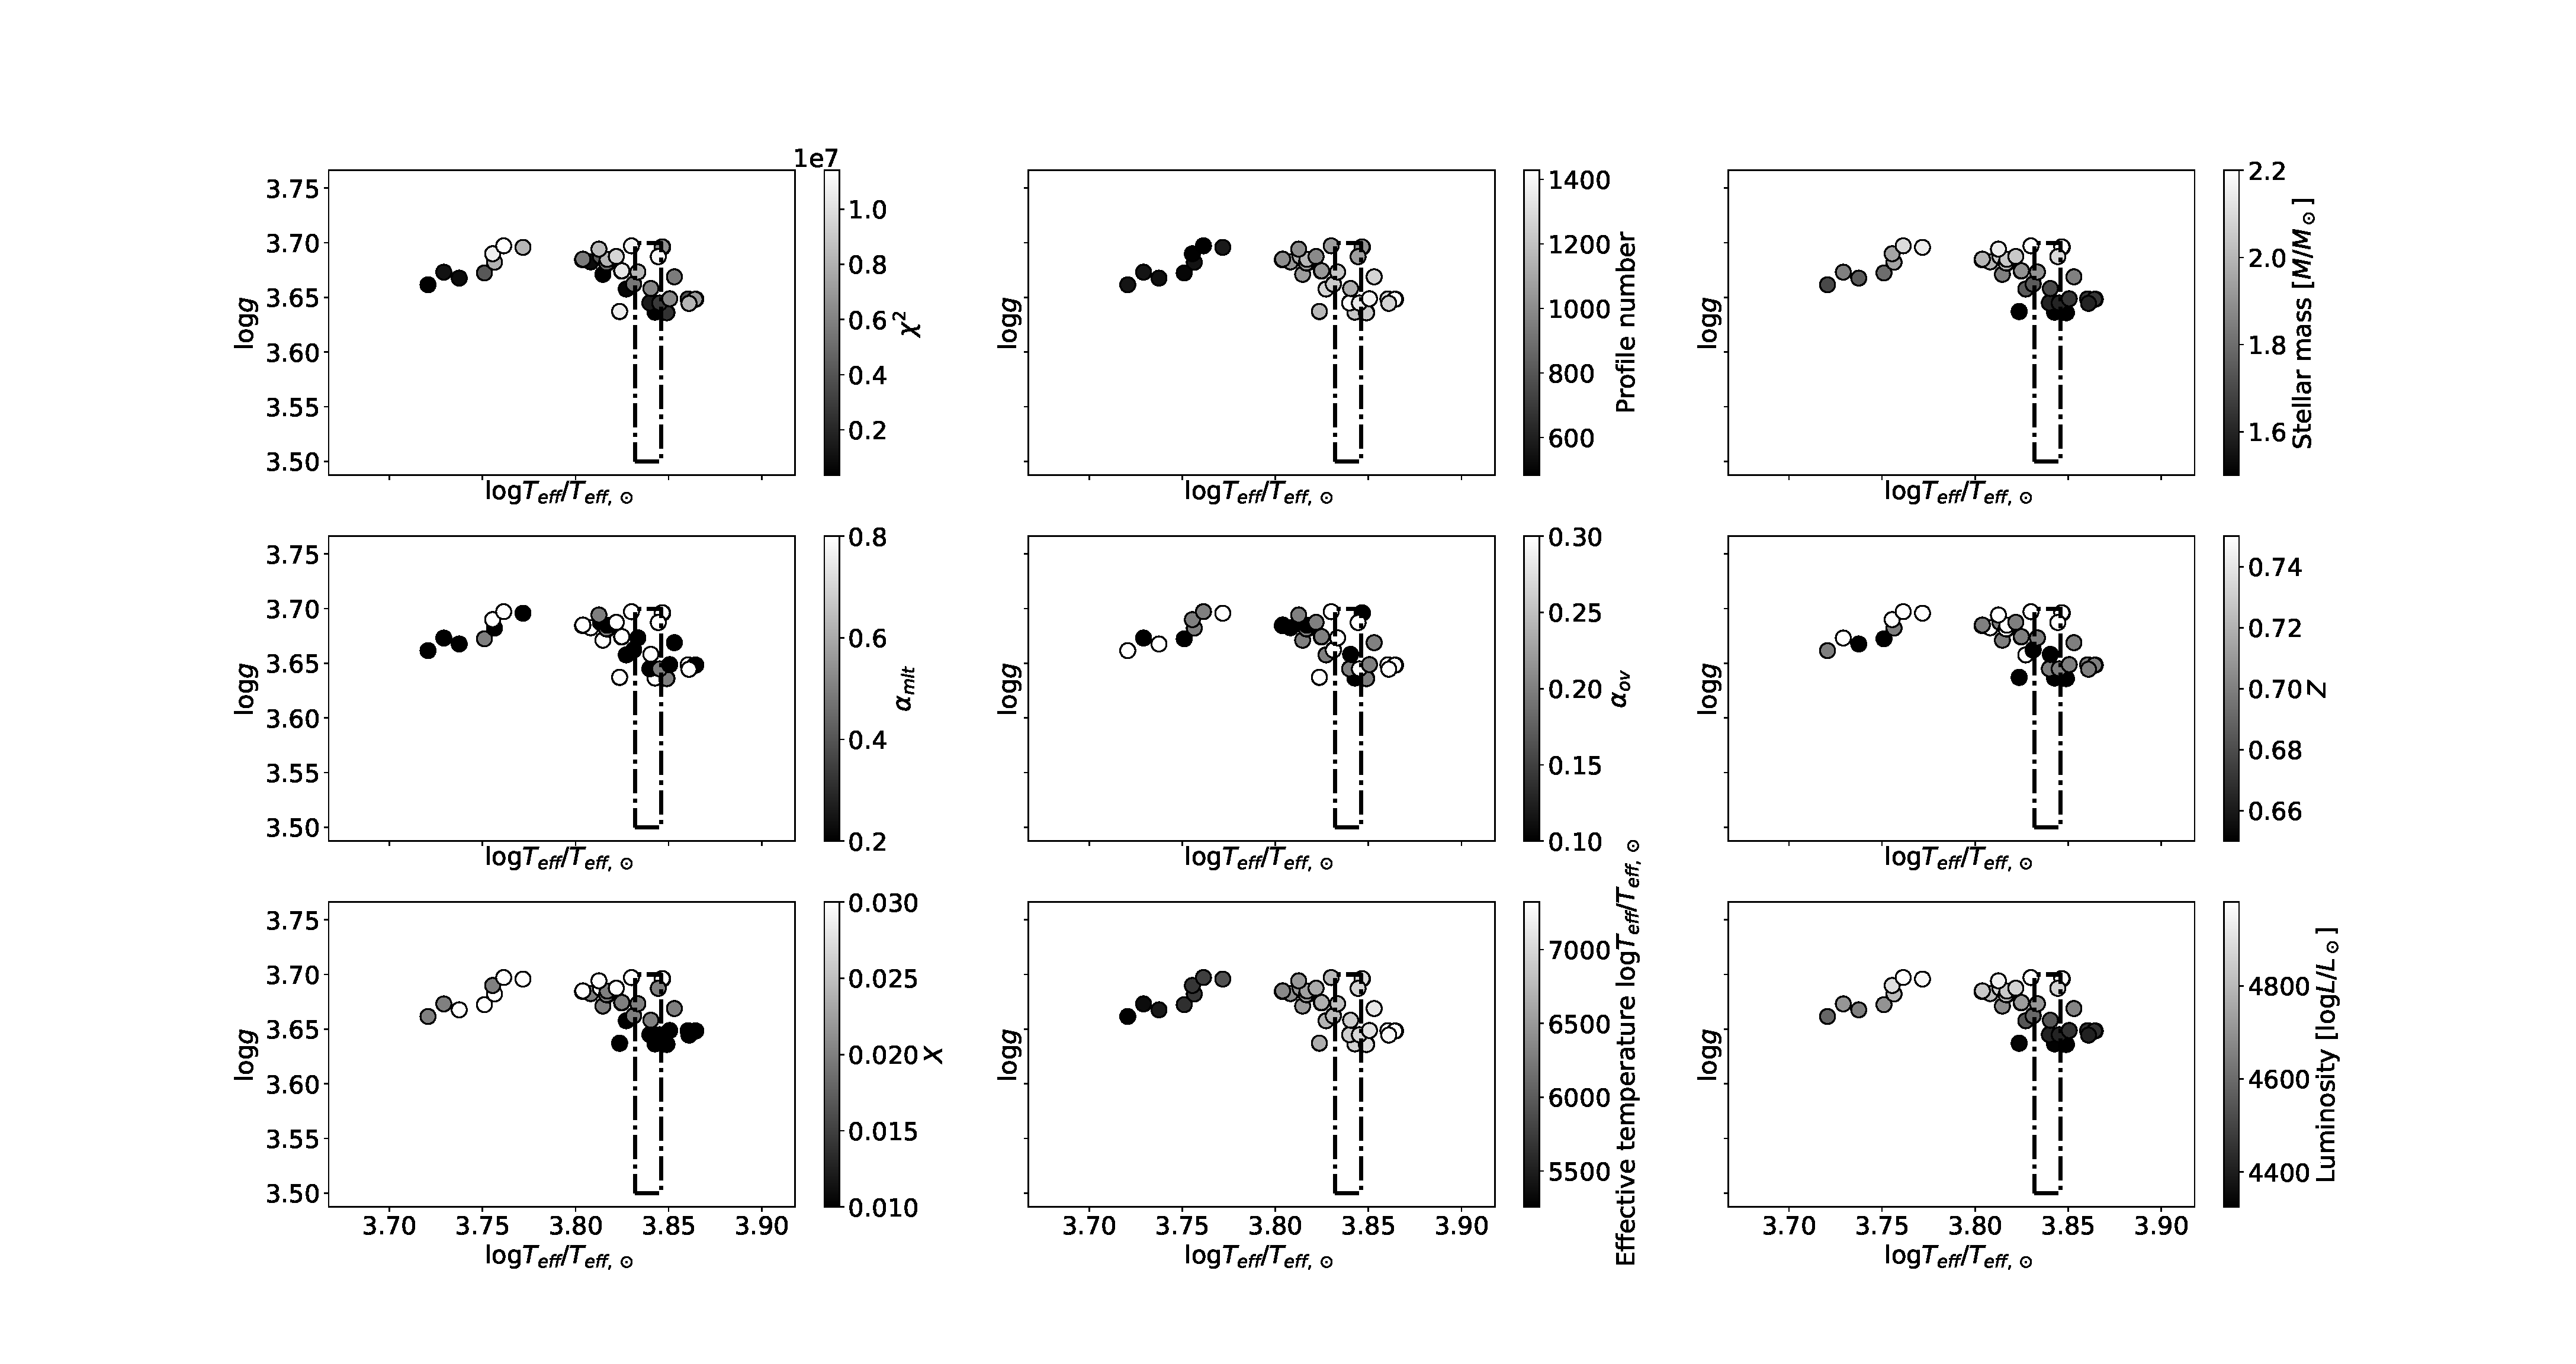
\includegraphics[width=1\textwidth]{scatter_all_v2.eps}
%	\makebox[\textwidth][c]{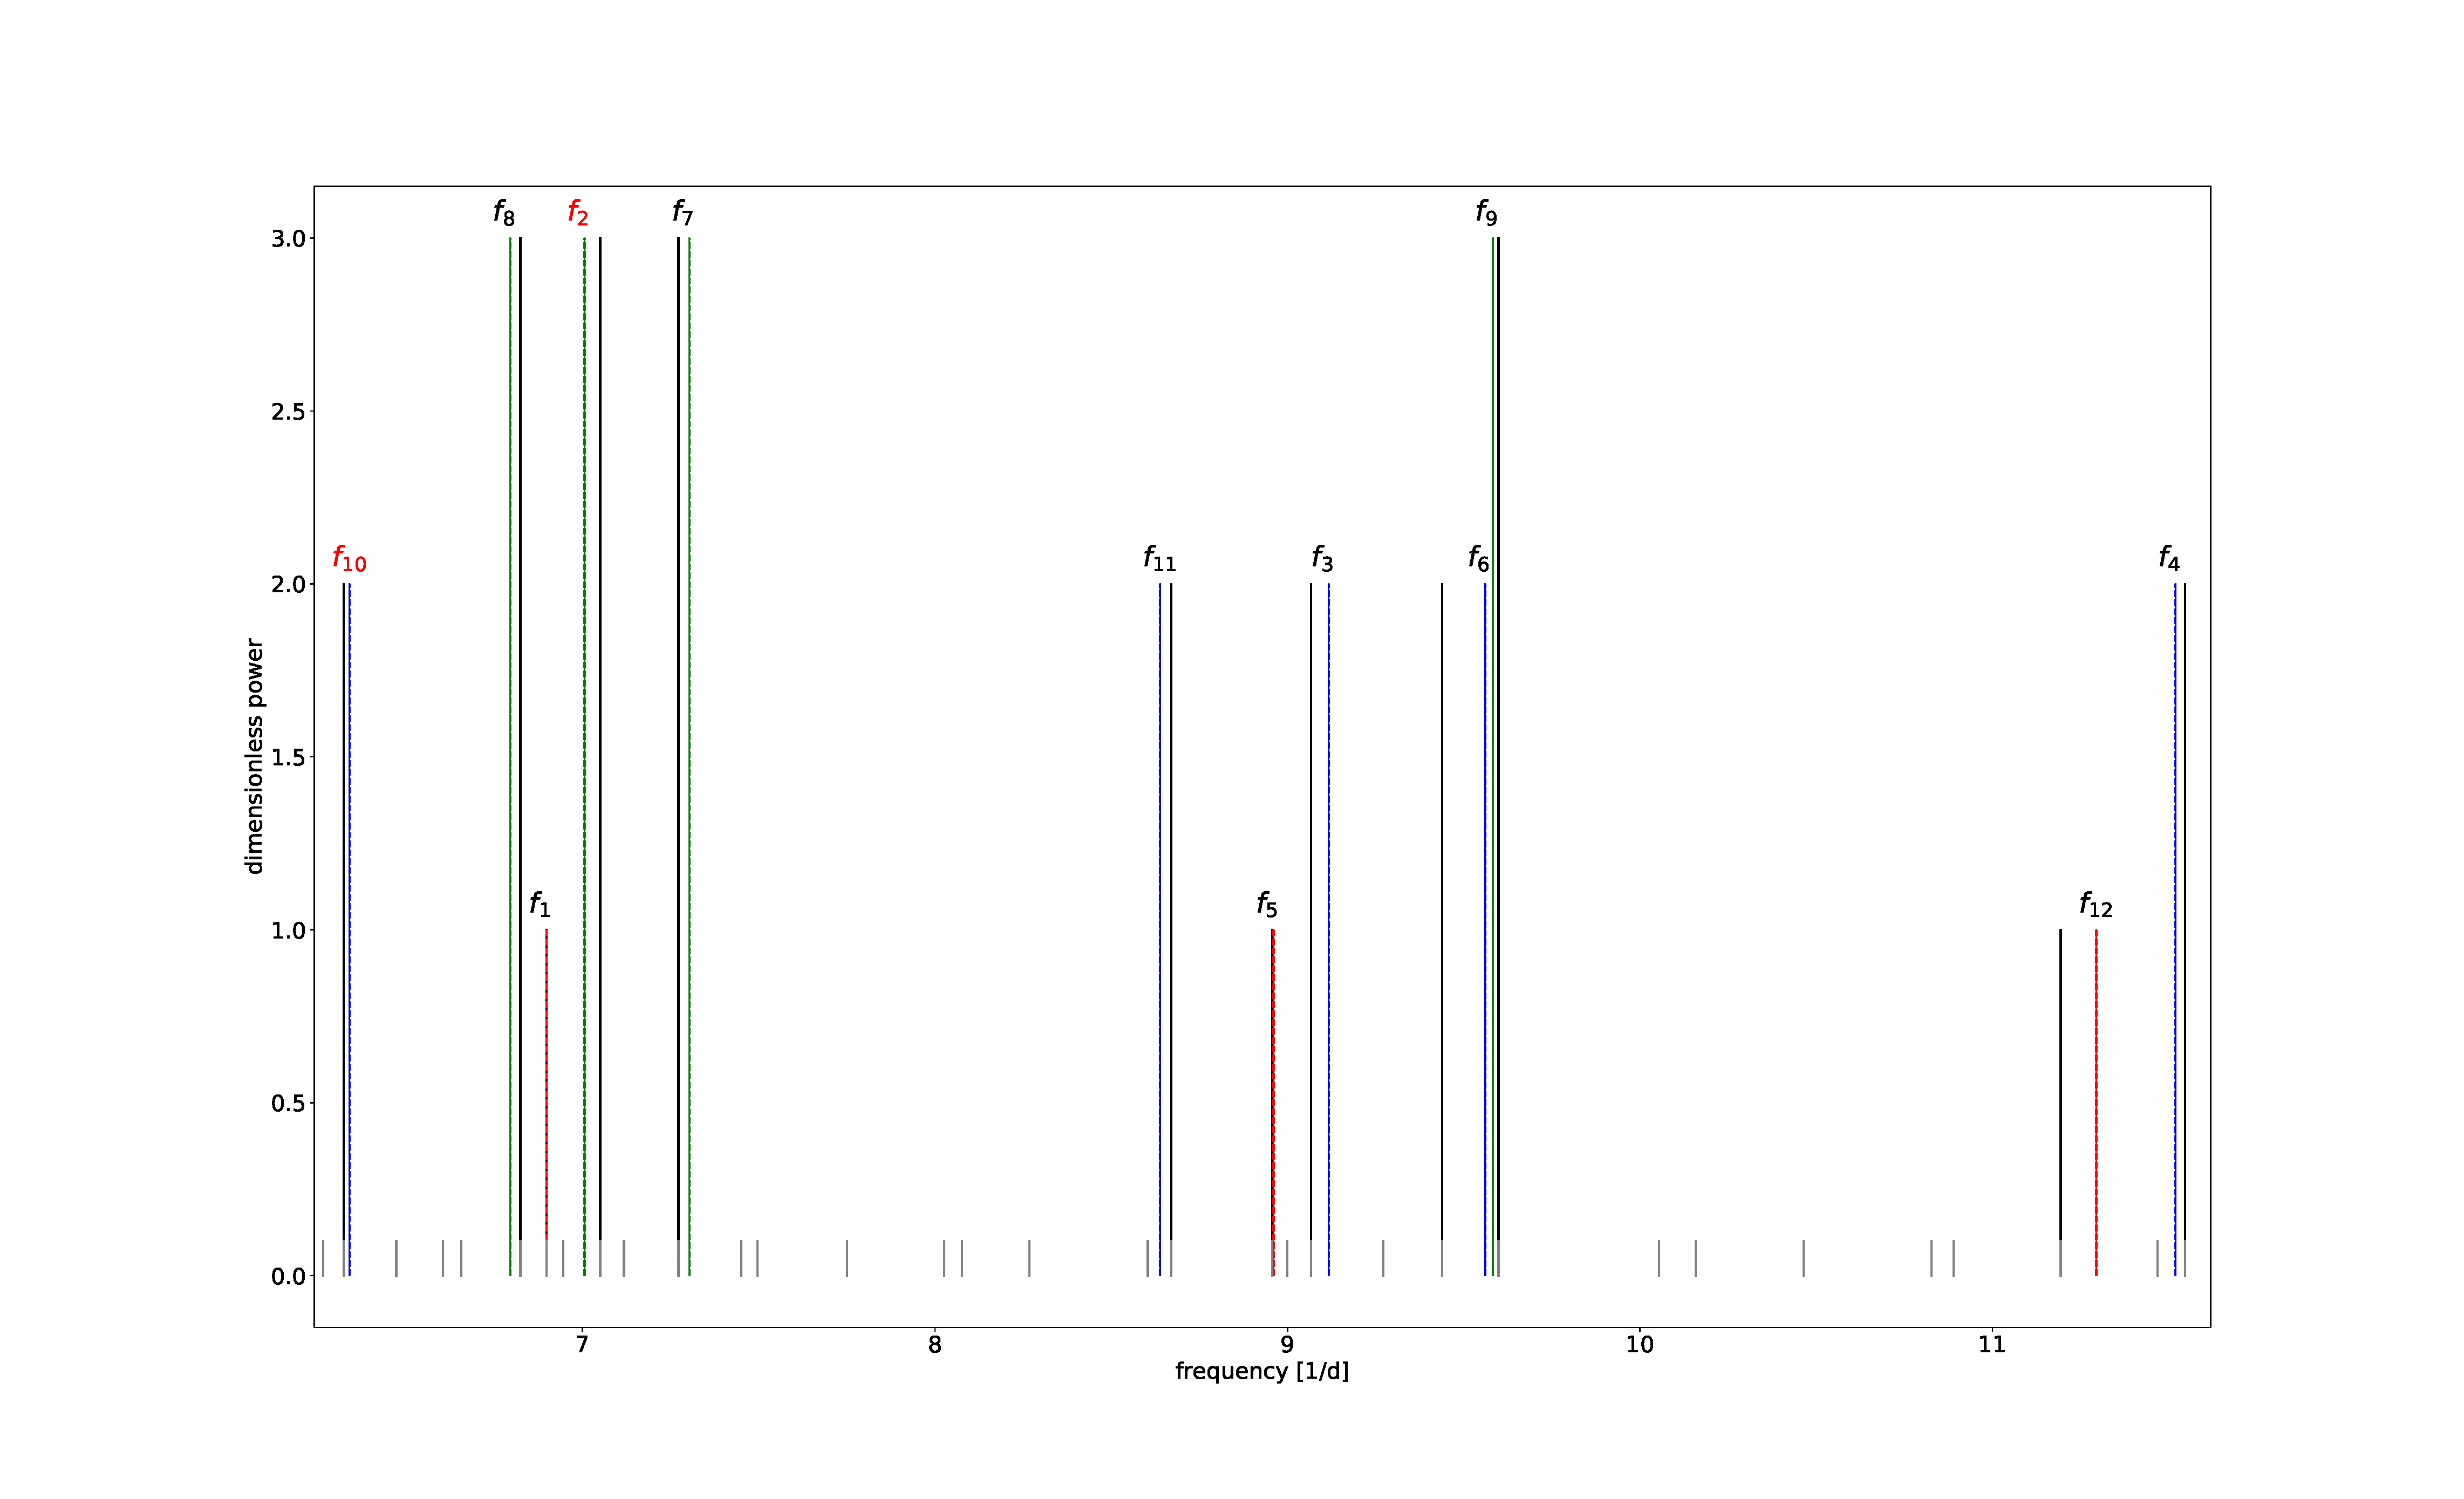
\includegraphics[width=1.5\textwidth]{frequency_fit.eps}}%
%	\caption{}
%	\label{}
%\end{figure}